% Customizable fields and text areas start with % >> below.
% Lines starting with the comment character (%) are normally removed before release outside the collaboration, but not those comments ending lines

% svn info. These are modified by svn at checkout time.
% The last version of these macros found before the maketitle will be the one on the front page,
% so only the main file is tracked.
% Do not edit by hand!
\RCS$Revision: 297494 $
\RCS$HeadURL: svn+ssh://nckw@svn.cern.ch/reps/tdr2/notes/EXO-12-055/trunk/EXO-12-055.tex $
\RCS$Id: EXO-12-055.tex 297494 2015-07-21 09:28:20Z nckw $
%%%%%%%%%%%%% local definitions %%%%%%%%%%%%%%%%%%%%%
% This allows for switching between one column and two column (cms@external) layouts
% The widths should  be modified for your particular figures. You'll need additional copies if you have more than one standard figure size.
\newlength\cmsFigWidth
\newcommand{\Zmm}{\ensuremath{Z\to\mu^+\mu^-}}
\newcommand{\Zvv}{\ensuremath{Z\to\nu\nu}}
\newcommand{\Wlv}{\ensuremath{W\to l\nu}}
\newcommand{\Zmmjets}{\ensuremath{Z(\mu\mu)+\textrm{jets}}}
\newcommand{\Zjets}{\ensuremath{Z+\textrm{jets}}}
\newcommand{\Zlljets}{\ensuremath{Z(ll)+\textrm{jets}}}
\newcommand{\Zvvjets}{\ensuremath{Z(\nu\nu)+\textrm{jets}}}
\newcommand{\Wlvjets}{\ensuremath{W(l\nu)+\textrm{jets}}}
\newcommand{\Wmvjets}{\ensuremath{W(\mu\nu)+\textrm{jets}}}
\newcommand{\phojets}{\ensuremath{\gamma+\textrm{jets}}}
\newcommand{\brhiggs}{\ensuremath{0.62}}
\newcommand{\higgsbr}{\ensuremath{0.62}}
\newcommand{\higgsbrobs}{\ensuremath{0.53}}
\newcommand\numberthis{\addtocounter{equation}{1}\tag{\theequation}}

\ifthenelse{\boolean{cms@external}}{\setlength\cmsFigWidth{0.85\columnwidth}}{\setlength\cmsFigWidth{0.4\textwidth}}
\ifthenelse{\boolean{cms@external}}{\providecommand{\cmsLeft}{top\xspace}}{\providecommand{\cmsLeft}{left\xspace}}
\ifthenelse{\boolean{cms@external}}{\providecommand{\cmsRight}{bottom\xspace}}{\providecommand{\cmsRight}{right\xspace}}
%%%%%%%%%%%%%%%  Title page %%%%%%%%%%%%%%%%%%%%%%%%
\cmsNoteHeader{EXO-12-055} % This is over-written in the CMS environment: useful as preprint no. for export versions
% >> Title: please make sure that the non-TeX equivalent is in PDFTitle below
\title{Search for Dark Matter in events with missing transverse momentum in association with jets or hadronically decaying vector bosons in pp collisions at $\sqrt{s}=8$ TeV
with the CMS detector.}

% >> Authors
%Author is always "The CMS Collaboration" for PAS and papers, so author, etc, below will be ignored in those cases
%For multiple affiliations, create an address entry for the combination
%To mark authors as primary, use the \author* form
\address[neu]{Northeastern University}
\address[fnal]{Fermilab}
\address[cern]{CERN}
\author[cern]{The CMS Collaboration}

% >> Date
% The date is in yyyy/mm/dd format. Today has been
% redefined to match, but if the date needs to be fixed, please write it in this fashion.
% For papers and PAS, \today is taken as the date the head file (this one) was last modified according to svn: see the RCS Id string above.
% For the final version it is best to "touch" the head file to make sure it has the latest date.
\date{\today}

% >> Abstract
% Abstract processing:
% 1. **DO NOT use \include or \input** to include the abstract: our abstract extractor will not search through other files than this one.
% 2. **DO NOT use %**                  to comment out sections of the abstract: the extractor will still grab those lines (and they won't be comments any longer!).
% 3. For PASs: **DO NOT use tex macros**         in the abstract: CDS MathJax processor used on the abstract doesn't understand them _and_ will only look within $$. The abstracts for papers are hand formatted so macros are okay.
\abstract{
A search is presented for an excess of events with a large missing transverse momentum in association with a highly energetic jet in a data sample of proton-proton 
interactions at centre-of-mass energy of 8TeV. The data correspond to an integrated luminosity of 19.7 $\textrm{fb}^{-1}$ collected by the CMS detector at the LHC.
Additional sensitivity is achieved by tagging events consistent with the jet originating from a boosted hadronically decaying vector boson.   
The results are interpreted as a set of a searches for a new scalar,
pseudoscalar, vector, and axial mediator that produces of dark
matter. 
}

% >> PDF Metadata
% Do not comment out the following hypersetup lines (metadata). They will disappear in NODRAFT mode and are needed by CDS.
% Also: make sure that the values of the metadata items are sensible and are in plain text:
% (1) no TeX! -- for \sqrt{s} use sqrt(s) -- this will show with extra quote marks in the draft version but is okay).
% (2) no %.
% (3) No curly braces {}.
\hypersetup{%
pdfauthor={CMS Collaboration},%
pdftitle={Search for Dark Matter in events with missing transverse energy in association with jets or hadronically decaying vector bosons in pp collisions at $\sqrt{s}=8 TeV$ 
with the CMS detector.},%
pdfsubject={CMS},%
pdfkeywords={CMS, physics, software, computing}}

\maketitle %maketitle comes after all the front information has been supplied
% >> Text
%%%%%%%%%%%%%%%%%%%%%%%%%%%%%%%%%%%%%%%%%%%%%%
%%%%%%%%%%%%%%%%%%%%%%%%%%%%%%%%%%%%%%%%%%%%%%
\section{Introduction}
%%%%%%%%%%%%%%%%%%%%%%%%%%%%%%%%%%%%%%%%%%%%%%
%%%%%%%%%%%%%%%%%%%%%%%%%%%%%%%%%%%%%%%%%%%%%%
This paper describes a search for Dark Matter (DM) in events containing an energetic narrow or wide jet and an imbalance of transverse momentum (\ETm) in a dataset 
of pp collisions provided by the Large Hadron Collider (LHC) at a centre-of-mass energy of 8 TeV. The data were collected using the Compact Muon Solenoid (CMS) 
detector and correspond to an integrated luminosity of 19.7\fbinv. 

The existence of Dark Matter is one of the most compelling sources of evidence for physics beyond the Standard Model (SM) with a number of astrophysical observations 
suggesting an abundance of a non-baryonic form of matter in the universe. In many theories which extend the SM, the production of DM particles in high-energy hadron-hadron 
collisions, such as those produced at the LHC is realised via a mediator which couples to both the SM and the DM particles.  
The ``monojet'' search provides a model-independent means of exploring DM production at the LHC~\cite{monojet1,monojet2} while 
 ``mono-V'', V=W or Z boson, searches~\cite{monolep,Aad:2014vka,Aad:2013oja,ATLAS:2014wra} target the associated production of DM with SM vector bosons, 
which can be enhanced in theories with non-universal DM couplings~\cite{IVDM}.  The interpretation of results from these and other DM searches at 
the LHC have generally utilized effective field theories (EFT) that assume heavy mediators and DM production via contact interactions~\cite{Fox:2011pm}.  
The results of this analysis are interpreted in the context of a spin-0, and spin-1 mediator decaying to Dark Matter deonted simplified DM models,~\cite{simplified1,Buchmueller:2013dya,Buchmueller:2014yoa}, compatible with the recent recommendation of the ATLAS-CMS LHC DM forum~\cite{Abercrombie:2015wmb}, which span a broad range of 
mediator and DM particle properties. This allows for a comparison in sensitivity with respect to direct detection experiments while retaining validity as a description of DM 
production across the entire kinematic region accessible at the LHC. 

This search is the first at CMS to target the hadronic decay modes of the vector bosons in the mono-V channels. A multivariate V-tagging technique is 
employed to identify the individual jets of moderately boosted vector bosons. The exploration of mono-V production at high boost 
utilises recently developed techniques designed to exploit information 
available in the sub-structure of jets. The events are categorised according to the nature of the jets in the event and the signal extraction is performed by 
considering the $\ETm$ distribution in each event category. These two features provide improved sensitivity compared to the previous CMS monojet analysis~\cite{monojet1}. 


%~\cite{Abercrombie:2015wmb}.

%The canonical ``monojet'' search strategy provides a model-independent means of exploring this scenario~\cite{monojet1,monojet2} while 
%related ``mono-V'' (V=W/Z) searches~\cite{monolep,monoZHbb} target the associated production of DM with SM vector bosons, 
%which can be enhanced in theories with non-universal DM couplings~\cite{IVDM}.  The interpretation of results from these and other DM searches at 
%the Large Hadron Collider (LHC) have generally utilized effective field theories (EFT) that assume heavy mediators and DM production via contact interactions~\cite{Fox:2011pm}.  

This paper is structured as follows; Section 2 outlines the Dark Matter models explored as signal hypotheses and Section 3 provides a 
description of the physics object reconstruction and the event selection and categorisation used in the search. Section 4 describes the 
background modelling used for the signal extraction. The results of this analysis and interpretations of the results in the context of 
simplified models for DM production are presented in Section 5.


%===============================================================================
\section{CMS detector}

The CMS detector, described in detail in ref.~\cite{CMSdetector}, is a multi-purpose apparatus designed to study high-$\pt$ physics processes in proton-proton and heavy-ion collisions.  
A superconducting solenoid occupies its central 
region, providing a magnetic field of 3.8\unit{T} parallel to the beam direction. Charged-particle trajectories are measured by the silicon pixel and strip trackers, which 
cover a pseudorapidity region of $\abs{\eta} < 2.5$. A lead tungstate (PbWO$_4$) crystal electromagnetic calorimeter (ECAL) and a brass/scintillator hadron calorimeter (HCAL) 
surround the tracking volume and cover $\abs{\eta} < 3$. The steel/quartz-fiber Cherenkov hadron forward (HF) calorimeter extends the coverage to $\abs{\eta} < 5$.  
The muon system consists of gas-ionization detectors embedded in the steel flux return yoke outside the solenoid, and covers $\abs{\eta} < 2.4$. The first level of the 
CMS trigger system, composed of custom hardware processors, is designed to select the most interesting events in less than 4\mus, using information from the calorimeters 
and muon detectors. The high-level trigger processor farm then further reduces the event rate to a few hundred Hz.

\section{Signal Hypotheses}
The signal hypotheses targeted in this search are provided under a set of simplified mediator models. These models assume an additional particle, 
a fermionic dark matter candidate, and an additional interaction that forces the production of a Dark Matter. 
It is assumed that this additional interaction is mediated by a generic spin-0 or spin-1 particle. 
The interactions are characterised by four distinct Lagrangians,
written for a Dirac-fermion Dark Matter particle $\chi$ with mass
$m_{DM}$ and mediator($S$,$P$,$Z'$,$Z''$) with mass $m_{MED}$ as, 

\begin{align}
\label{eq:LS} 
\mathcal{L}_{\mathrm{scalar}}&\supset\, -\,\frac{1}{2}m_{\rm MED}^2 S^2 - g_{\rm DM}  S \, \bar{\chi}\chi
 - \sum_{q=b,t} g_{SM}^q S \, \bar{q}q  - m_{\rm DM} \bar{\chi}\chi \,,
 \\
 \label{eq:LP} 
\mathcal{L}_{\rm{pseudoscalar}}&\supset\, -\,\frac{1}{2}m_{\rm MED}^2 P^2 - i g_{\rm DM}  P \, \bar{\chi} \gamma^5\chi
 -\sum_{q=b,t}  i g_{SM}^q  P \, \bar{q}  \gamma^5q  - m_{\rm DM} \bar{\chi}\chi\,,
 \\
 \label{eq:LV} 
\mathcal{L}_{\mathrm{vector}}&\supset \, \frac{1}{2}m_{\rm MED}^2 Z'_{\mu} Z'^{\mu} - g_{\rm DM}Z'_{\mu} \bar{\chi}\gamma^{\mu}\chi -\sum_q g_{SM}^q Z'_{\mu} \bar{q}\gamma^{\mu}q - m_{\rm DM} \bar{\chi}\chi\,,
 \\
 \label{eq:LA} 
\mathcal{L}_{\rm{axial-vector}}&\supset\,  \frac{1}{2}m_{\rm MED}^2 Z''_{\mu} Z''^{\mu} - g_{\rm DM} Z''_{\mu} \bar{\chi}\gamma^{\mu}\gamma^5\chi -\sum_q g_{SM}^q Z''_{\mu} \bar{q}\gamma^{\mu}\gamma^5q - m_{\rm DM} \bar{\chi}\chi\,
\end{align}

assuming pure scalar, pseudoscalar, vector, and axial-vector mediated interactions denoted by $S,~P,~Z'$ and $Z''$ mediators respectively. 
The couplings $g_{DM}$ and $g_{SM}$ denotes the coupling of the mediator to the Dark Matter particle and to standard model particles respectively. 
The choice of the split in terms of axial-vector and vector mediators in the Lagrangian is to parallel the existing separation with direct detection, into spin-dependent and spin-independent interactions. Here, spin-independent can refer to either vector or scalar mediated interactions, between which direct detection makes no distinction, while 
spin-dependent interactions refer to axial-vector mediated processes.
 
Pseudoscalar interactions are velocity suppressed in DM-nucleon interactions and thus limited sensitivity from the direct detection experiments is expected~\cite{Haisch:2012kf}. 
An extension to the scalar and pseudo-scalar can be performed by
allowing the scalar and pseudoscalar interactions to undergo electroweak symmetry breaking (EWSB) in an analogous way to 
the Higgs mechanism~\cite{Khoze:2015sra,Hambye:2013sna,Khoze:2014xha,Khoze:2014woa,Altmannshofer:2014vra,Carone:2013wla,Heikinheimo:2013fta}. Scalar and pseudoscalar models 
where EWSB is not present are denoted herein as \emph{fermionic} Dark Matter production.

In collider experiments, the production of Dark Matter in spin-0 mediated interactions is predominantly through gluon-fusion via a top-quark loop (see Figure~\ref{fig:monojet0}). 
When EWSB is present in the model, mono-V signatures are produced through a Higgs-strahlung like 
process (see Figure~\ref{fig:monoV0}). For the spin-1 signatures, Dark Matter is produced in an analogous way to Z boson production through quark initiated processes. The mono-V or monojet signatures follow 
from the presence of a radiated V-boson or jet in the initial state. In all models, the coupling of the mediator to standard model coupling is taken as unity 
($g_{SM}=1$) along with 
the Dark Matter coupling ($g_{DM}=1$). For the scalar and pseudoscalar models, this denotes a Yukawa coupling to standard model particles. For all models considered, 
the width is fixed under the minimum width constraint requiring that
only quarks and the dark matter couple to the mediator with no
additional modifications~\cite{Harris:2014hga}.

In order to model the expected contribution from these signals, Monte Carlo (MC) events are generated using MCFM~\cite{mcfm}
for the monojet final state, and JHUGen~\cite{Anderson:2013afp} 
for the vector boson final state. All signal models are 
generated at leading order, showered with Pythia6~\cite{Sjostrand:2006za} and passed through a 
simulation of the CMS detector using Geant4~\cite{geant4}. 
For scalar and pseudoscalar mediated DM production, the finite top
quark mass is taken into account. 

\begin{figure}[htbp]
  \centering
  \subfloat[][]{
        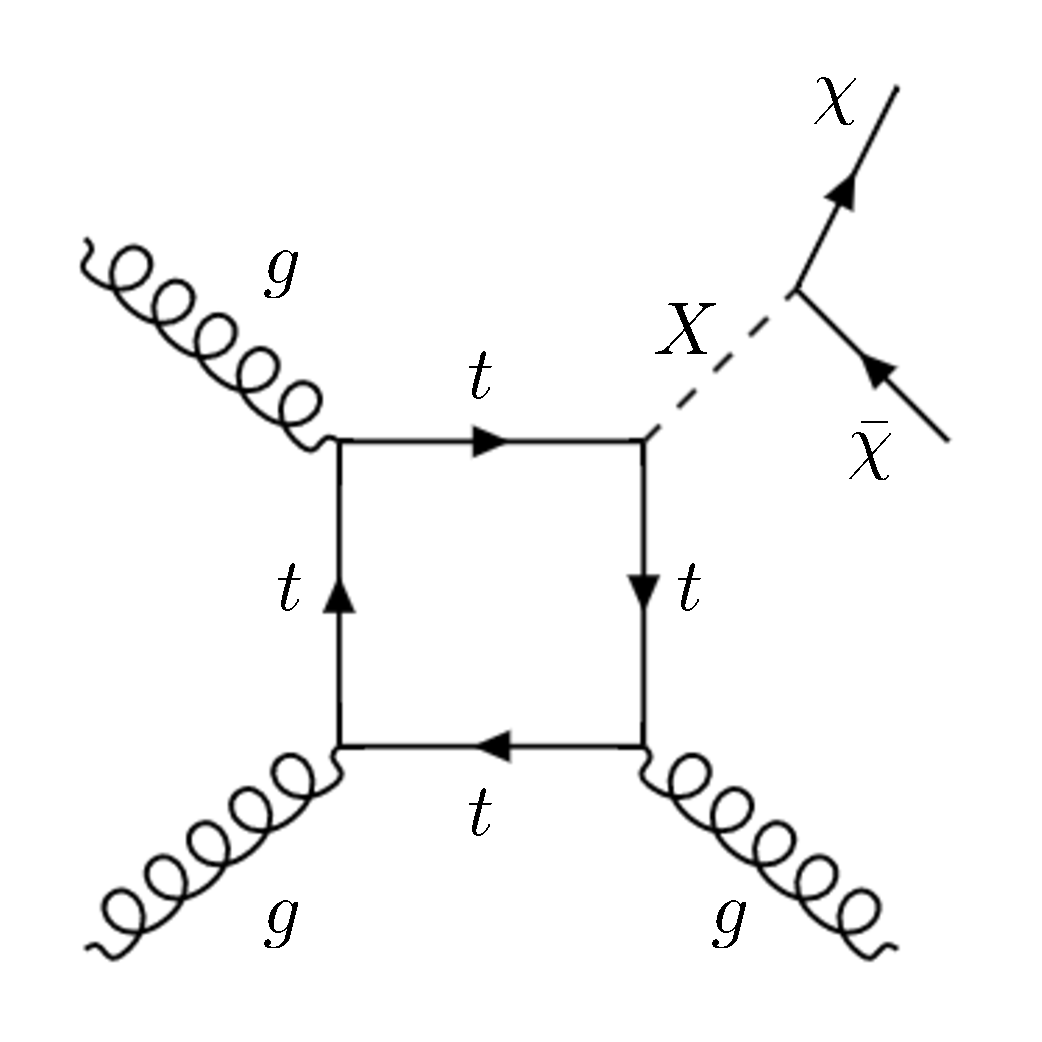
\includegraphics[angle=0,width=0.36\textwidth]{figures/scalarbox.pdf}
        \label{fig:monojet0}
  }
  \subfloat[][]{
        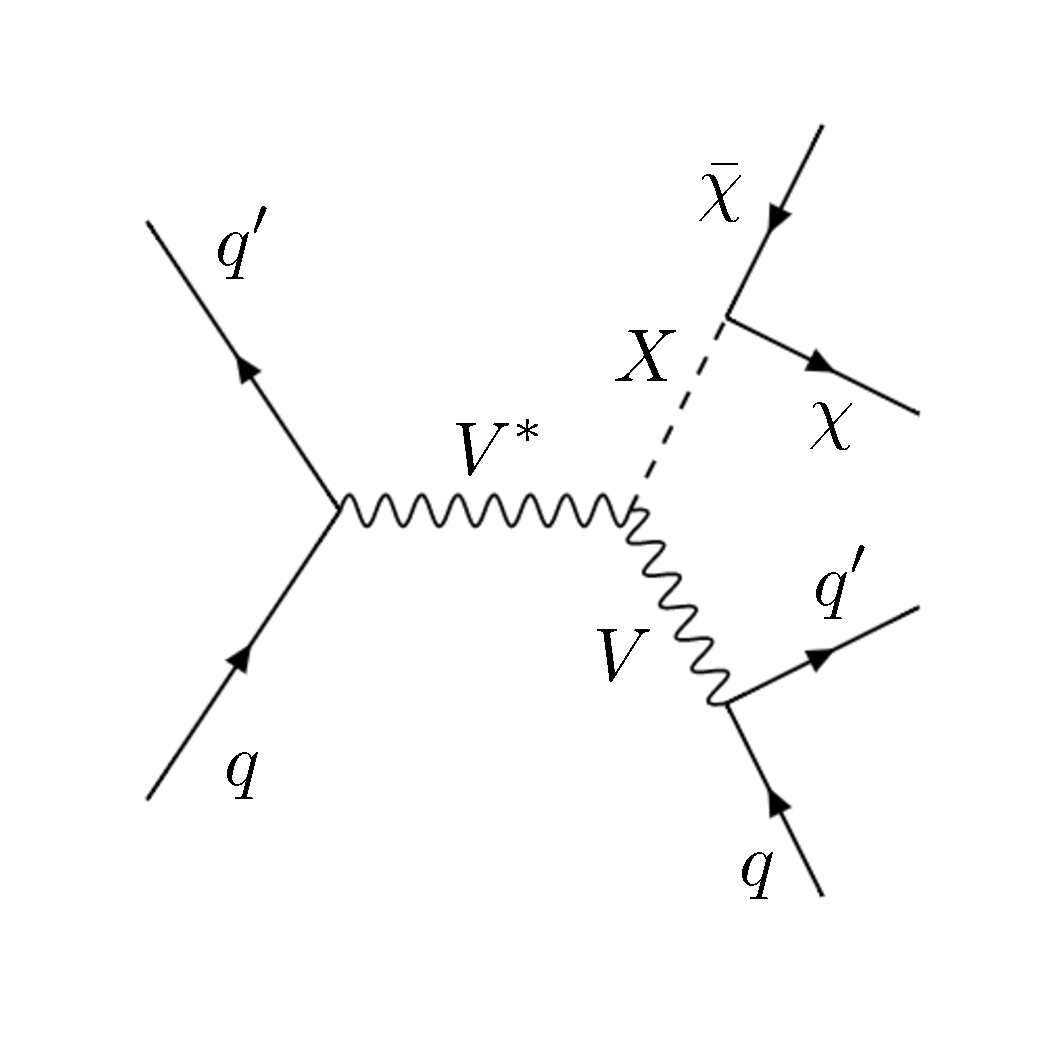
\includegraphics[angle=0,width=0.36\textwidth]{figures/scalarV.pdf}
        \label{fig:monoV0}
  }
  \caption{Diagrams for production of the monojet (a) and mono-V signature through Higgs-strahlung (b), through a scalar mediator.\label{fig:monoXfeyn}}
\end{figure}




\section{Event Selection and Categorization}\label{sec:selection}

Signal events are selected on the basis of large values of \ETm and one or more high-\pt jet(s), 
explicitly vetoing isolated leptons and photons. Events are
reconstructed with the CMS detector, following the standard CMS reconstruction~\cite{CMSdetector}. 

The data used for this analysis are collected using either of two triggers designed to record events containing large \ETm. The first requires an \ETm of greater than 120 \gev, calculated only using information from the calorimeter, 
while the second requires an \ETm greater than 95~\gev or 105~\gev, depending on the data-taking period, calculated using  
the particle flow (PF) reconstruction algorithm~\cite{CMS-PAS-PFT-09-001} as well as jet with \pt$>80$ \gev and $|\eta|<2.6$. 
The lowest threshold on the \ETm for the selection of the events is set at 200 \gev in order to maintain a trigger efficiency greater than 
$99$\% with respect to the full event selection. 

Jets are reconstructed from the clustering of PF objects using either the 
anti-$k_{\textrm{T}}$ algorithm~\cite{Cacciari:2008gp} with 0.5 (ak5 jet) as the distance parameter,  
or the Cambridge/Aachen algorithm~\cite{cajets} with 0.8 distance
parameter (ca8). The leading jet is further required to be well
identified, using a standard set of identification criteria~\cite{jec}. The jets are corrected for pileup on the basis of the event energy density and 
proportionally to their area. Data-driven calibrations are then applied to correct the absolute scale of the jet energy~\cite{jec}.

The \ETm is calculated as the magnitude of the negative 
vector sum of the transverse momenta of all final state particles, which are reconstructed 
using the particle-flow (PF) algorithm~\cite{CMS-PAS-PFT-09-001}.
Events with a large mis-reconstructed offline \ETm are removed by applying quality filters. 
The angle between the \ETm and the leading jet in the plane transverse to the beam line, $\Delta\phi$, is required to be larger than 2 to reduce the contribution from multijet QCD events. 
Finally, events are vetoed if they contain at least one well-identified and isolated electron, photon or muon with $p_T>10$~\gev, or a tau with $p_T>15$~\gev.

Selected events are classified into three event categories, based on the topology of the jets, in order to distinguish between 
initial or final state radiation of gluons or quarks and jets arising from hadronic vector boson decays.
The categories are first scrutinized for the presence of an unresolved
vector boson (boosted category), subsequently for a resolved vector
boson (resolved category), and finally the remaining events are collected into the monojet category. 

If the vector boson decays hadronically and has sufficiently high transverse momentum, both its hadronic
decay products are captured by a single reconstructed ``fat''-jet.
Events in the boosted vector boson category are required to
have a reconstructed ca8 jet with $\pt>200$ \gev and  $\ETm>250$ \gev.  Further cuts are applied to improve the vector boson jet
purity by cutting on the variable ``N-subjettiness'' ($\tau_2/\tau_1$ defined in~\cite{Thaler:2010tr,Thaler:2011gf}), which identifies jets with a 
two sub-jet topology, and the pruned jet mass~\cite{Ellis:2009me}. The $\tau_2/\tau_1$ ratio
is required to be smaller than 0.5 and the pruned jet mass, $m_{\mathrm{prune}}$, is selected to
be close to both the W and Z boson masses, namely to satisfy $60<m_{\mathrm{prune}}<110$ \gev.   
Events which contain additional jets close to the ca8 jet, but no closer than $\Delta R < 0.5$,
are selected to include the frequent cases in which initial state radiation yields additional jets. 
If an ak5 jet with $p_T>30$ and $|\eta|<2.5$ is reconstructed, and the opening angle between it 
and the ca8 jet, $\Delta\phi(\mathrm{ak5,ca8})$, is smaller than 2, the event is selected. Events with more than one ak5 jets 
with $p_T>30$ \gev and $|\eta|<2.5$, reconstructed at $\Delta R> 0.5$ with respect to the ca8 jet 
are rejected.
Figure~\ref{fig:boostvtagvars} shows the distributions of $\tau_2/\tau_1$ and $m_{\mathrm{prune}}$, (before the application 
of the jet mass cut) in simulation and data for the boosted event category. Some disagreement is present in the modelling between data and Monte Carlo simulation. This disagreement is well covered by the systematic uncertainties used in the analysis. A detailed discussion of the modelling can be found in ~\cite{Khachatryan:2014vla}.  
\begin{figure*}[hbtp]\begin{center}
\subfigure[]{
 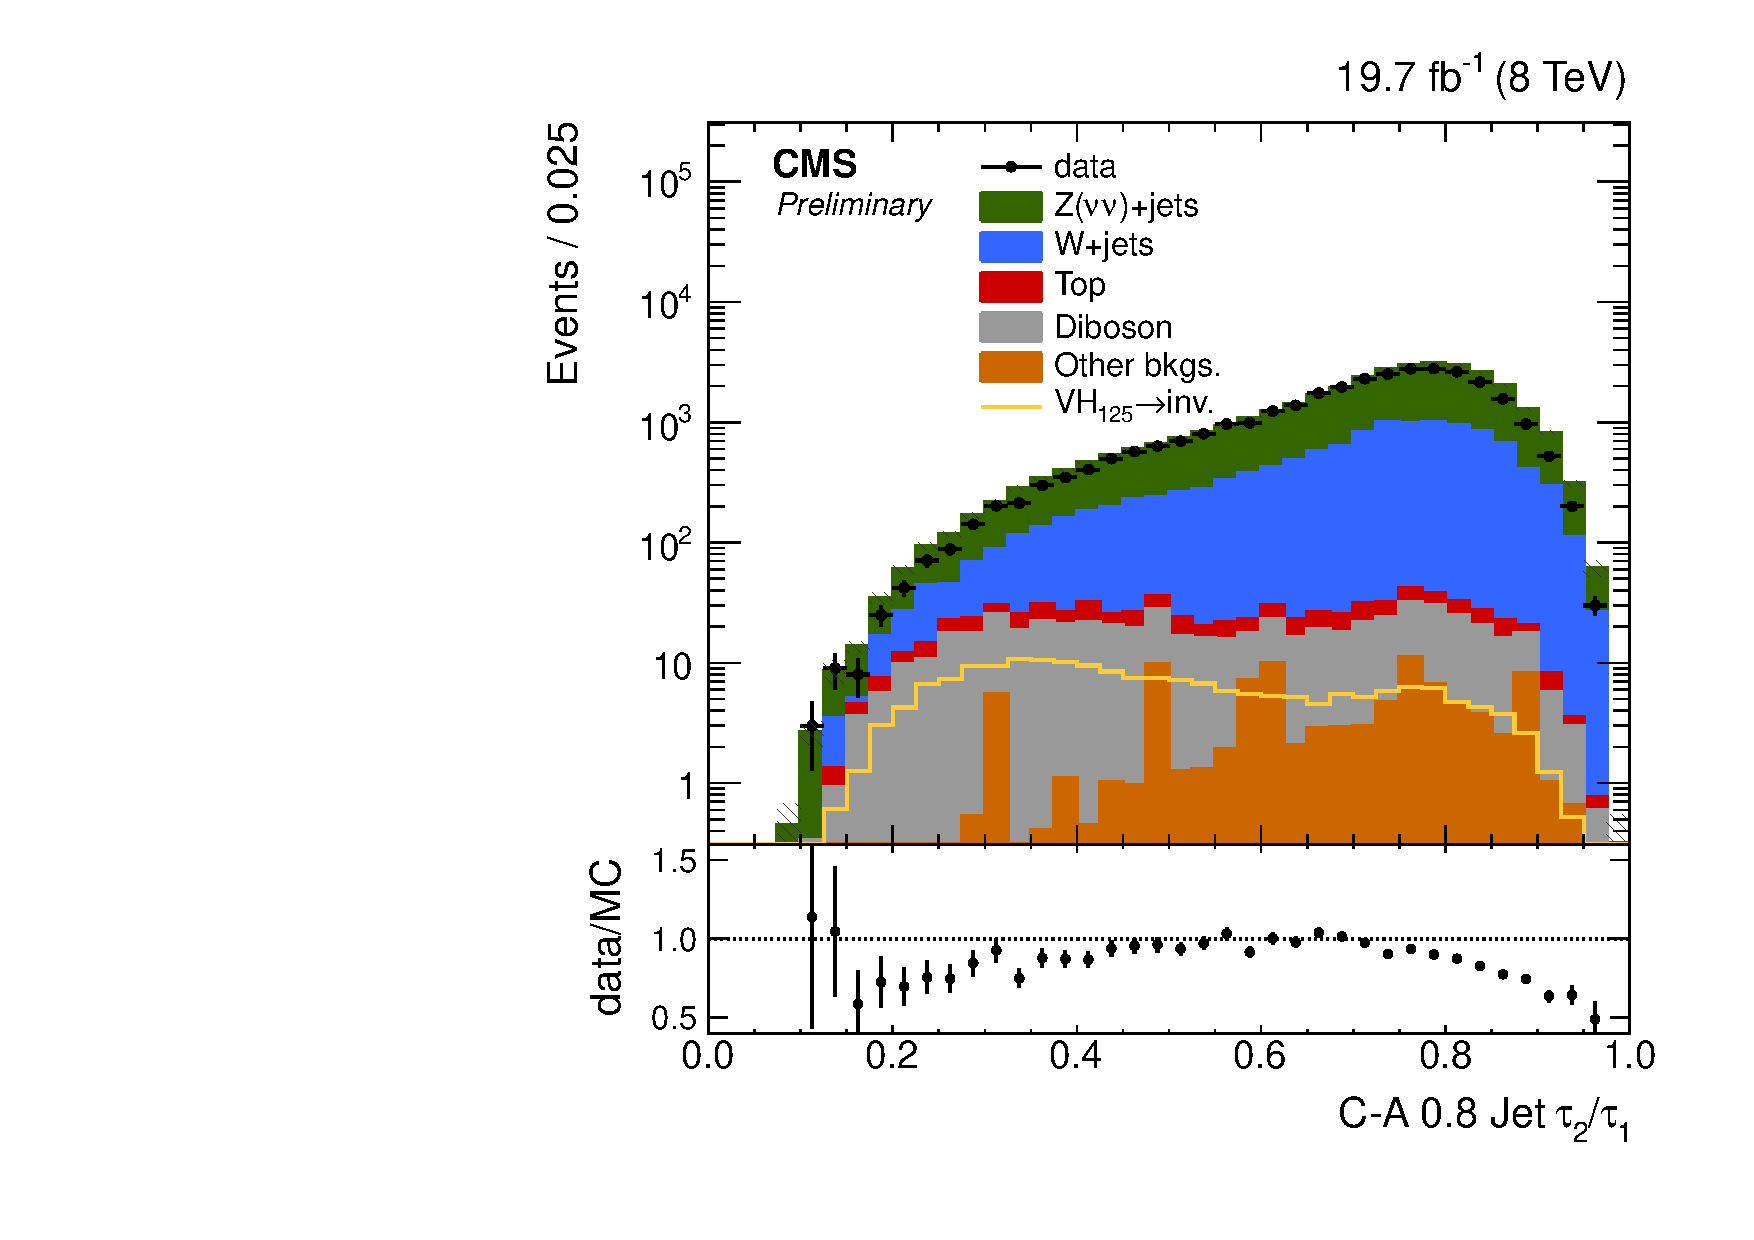
\includegraphics[width=0.49\textwidth]{figures/t2t1_sig_baseline.pdf}
}
\subfigure[]{
 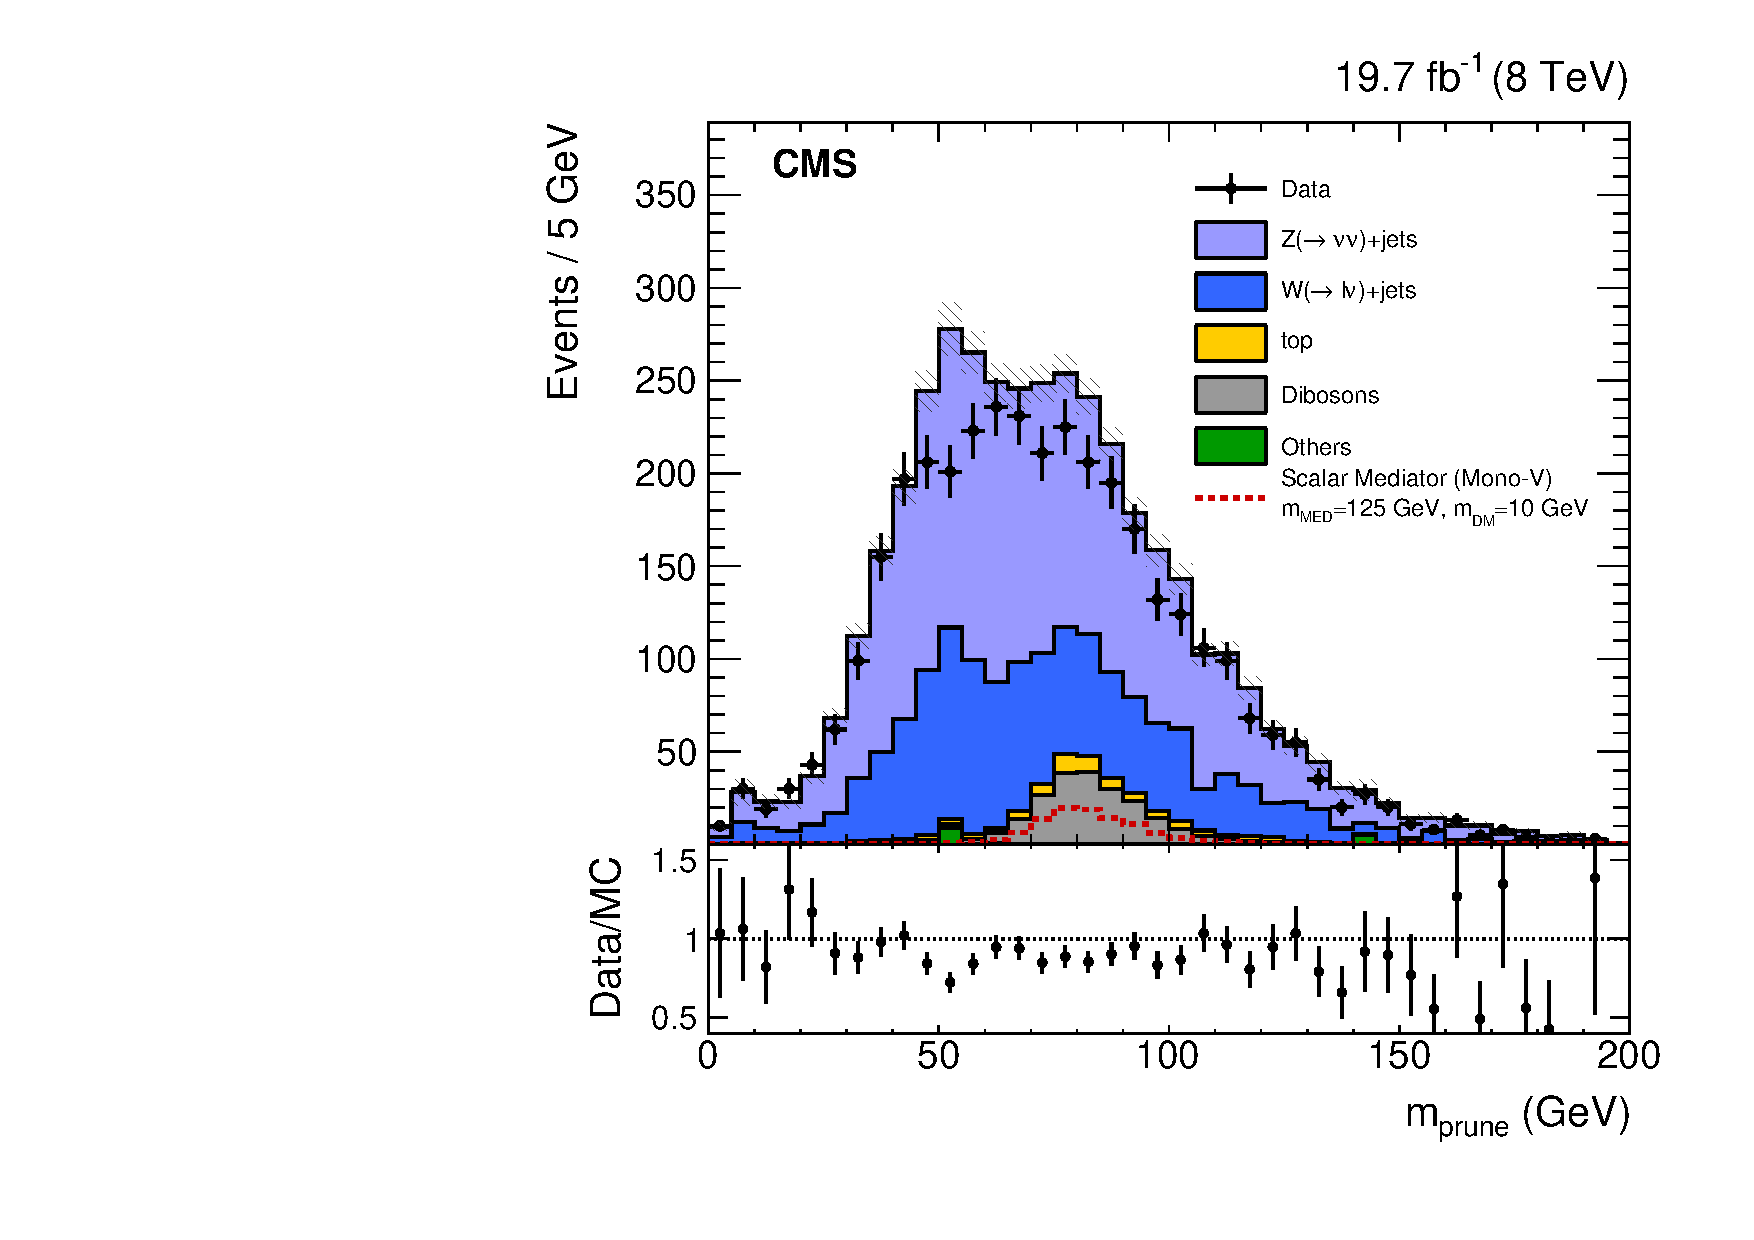
\includegraphics[width=0.49\textwidth]{figures/mass_sig_nomasscut.pdf}
}
 \caption{Distributions of $\tau_2/\tau_1$ before the jet mass cut (a) and pruned jet mass (b) for events in data and MC in the boosted event category. 
 A cut of $\tau_2/\tau_1<$0.5 has been applied in figure b.}
 \label{fig:boostvtagvars}\end{center}\end{figure*}

%\subsection{Resolved V-tagged category}\label{sec:resvtagging}
In cases where the electroweak boson has insufficient transverse momentum for its hadronic
decay to be fully contained in a single reconstructed fat-jet, a selection that looks for decays 
into a pair of ak5 jets is applied to recover the event. 
The selection requires that each jet has $p_T>30$ GeV and $|\eta|<2.5$ and that the dijet has a mass between 60\gev and 110\gev, consistent with originating 
from a W or Z boson. To further reduce the combinatorial background, a
multivariate V-tagger is applied. The inputs to this resolved V-tagger are the values from each jet of likelihood-based discriminator variable 
which distinguishes quark-initiated jets from gluon-initiated
jets~\cite{JME-14-002}, the jet pull angle~\cite{Gallicchio:2010sw}
and the mass drop variable~\cite{Izaguirre:2014ira}. In events 
where multiple dijet pairs are found, the pair with the highest V-tagger value is taken as the candidate. The distribution of the V-tagger variable for SM backgrounds and for a scalar mediator
produced in association with either a W or Z boson is shown in Figure~\ref{fig:vtagger}.
\begin{figure*}[hbtp]\begin{center}
  \subfloat[][]{
 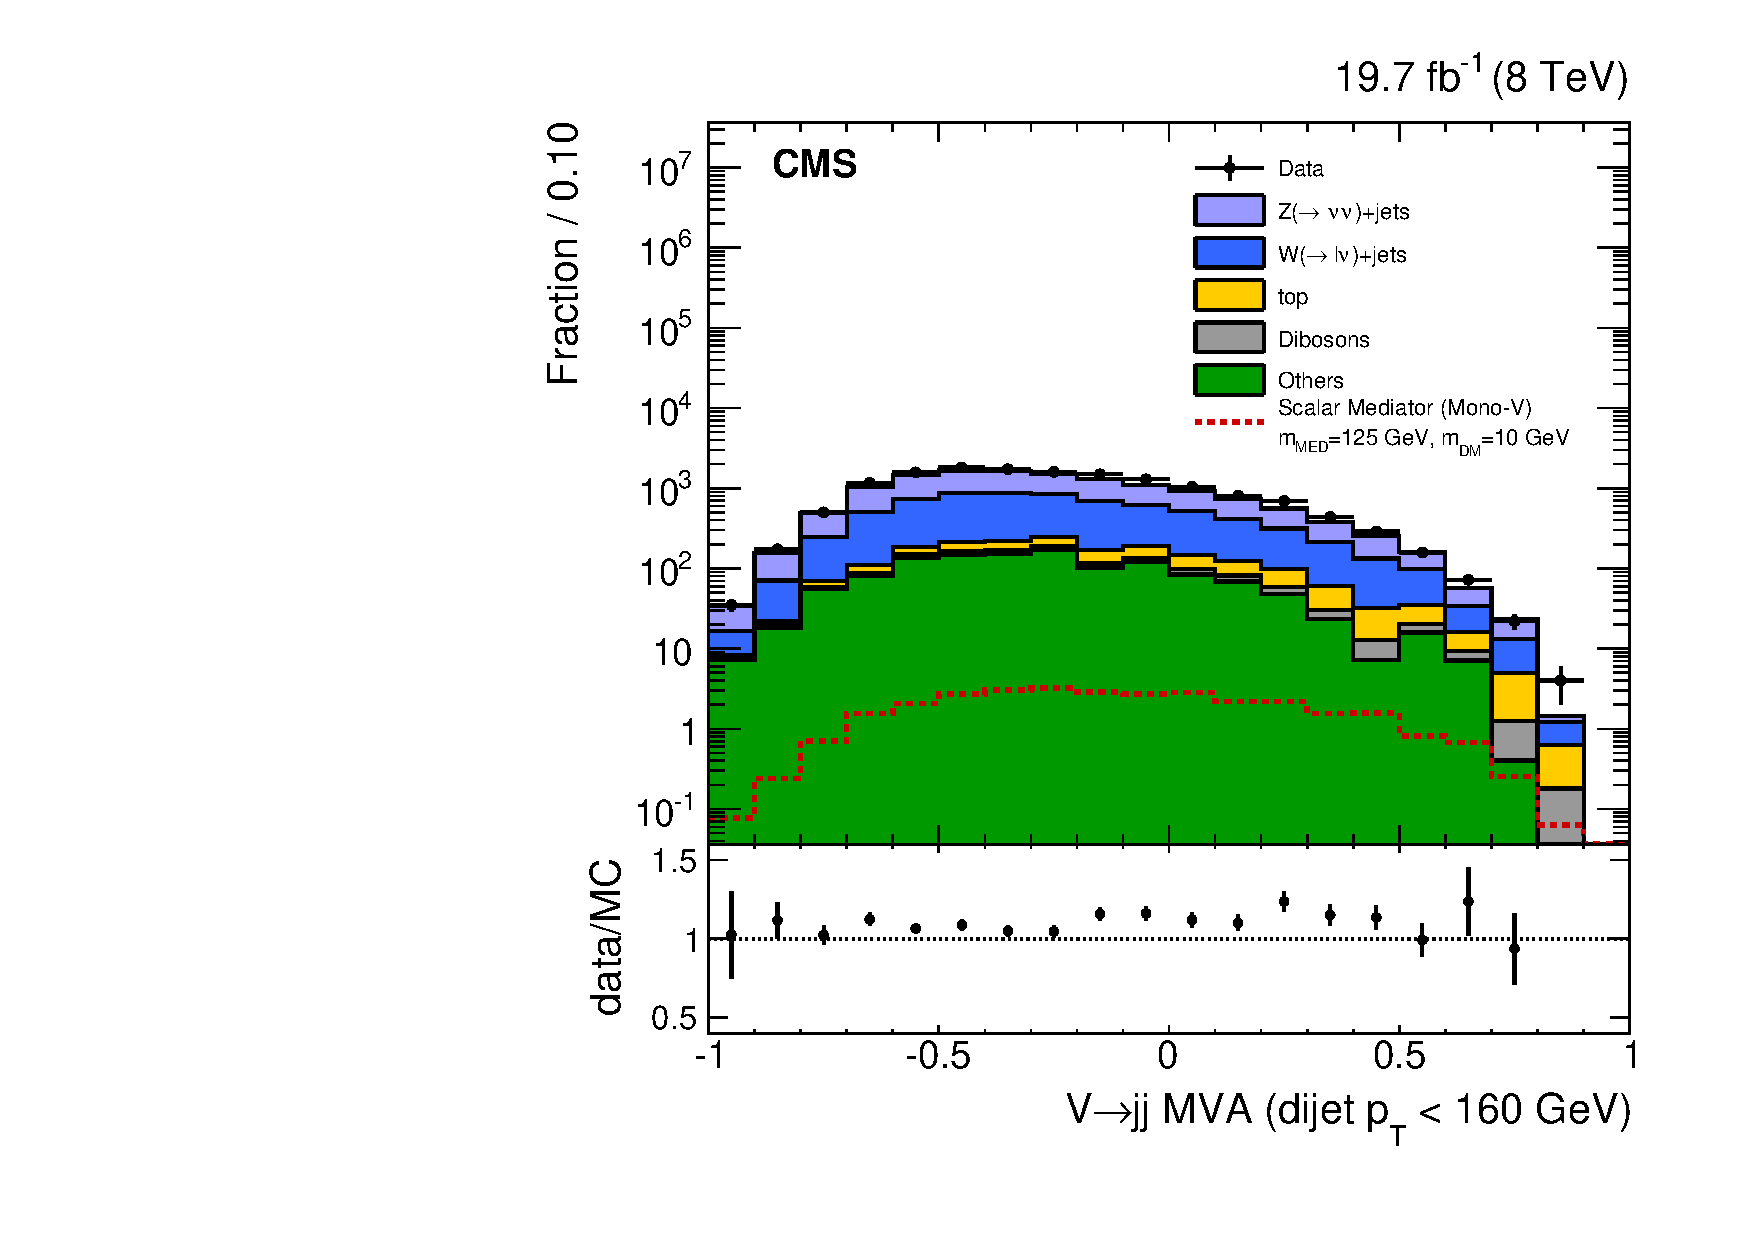
\includegraphics[width=0.49\textwidth]{figures/res_vmvalog_0.pdf}
}
  \subfloat[][]{
 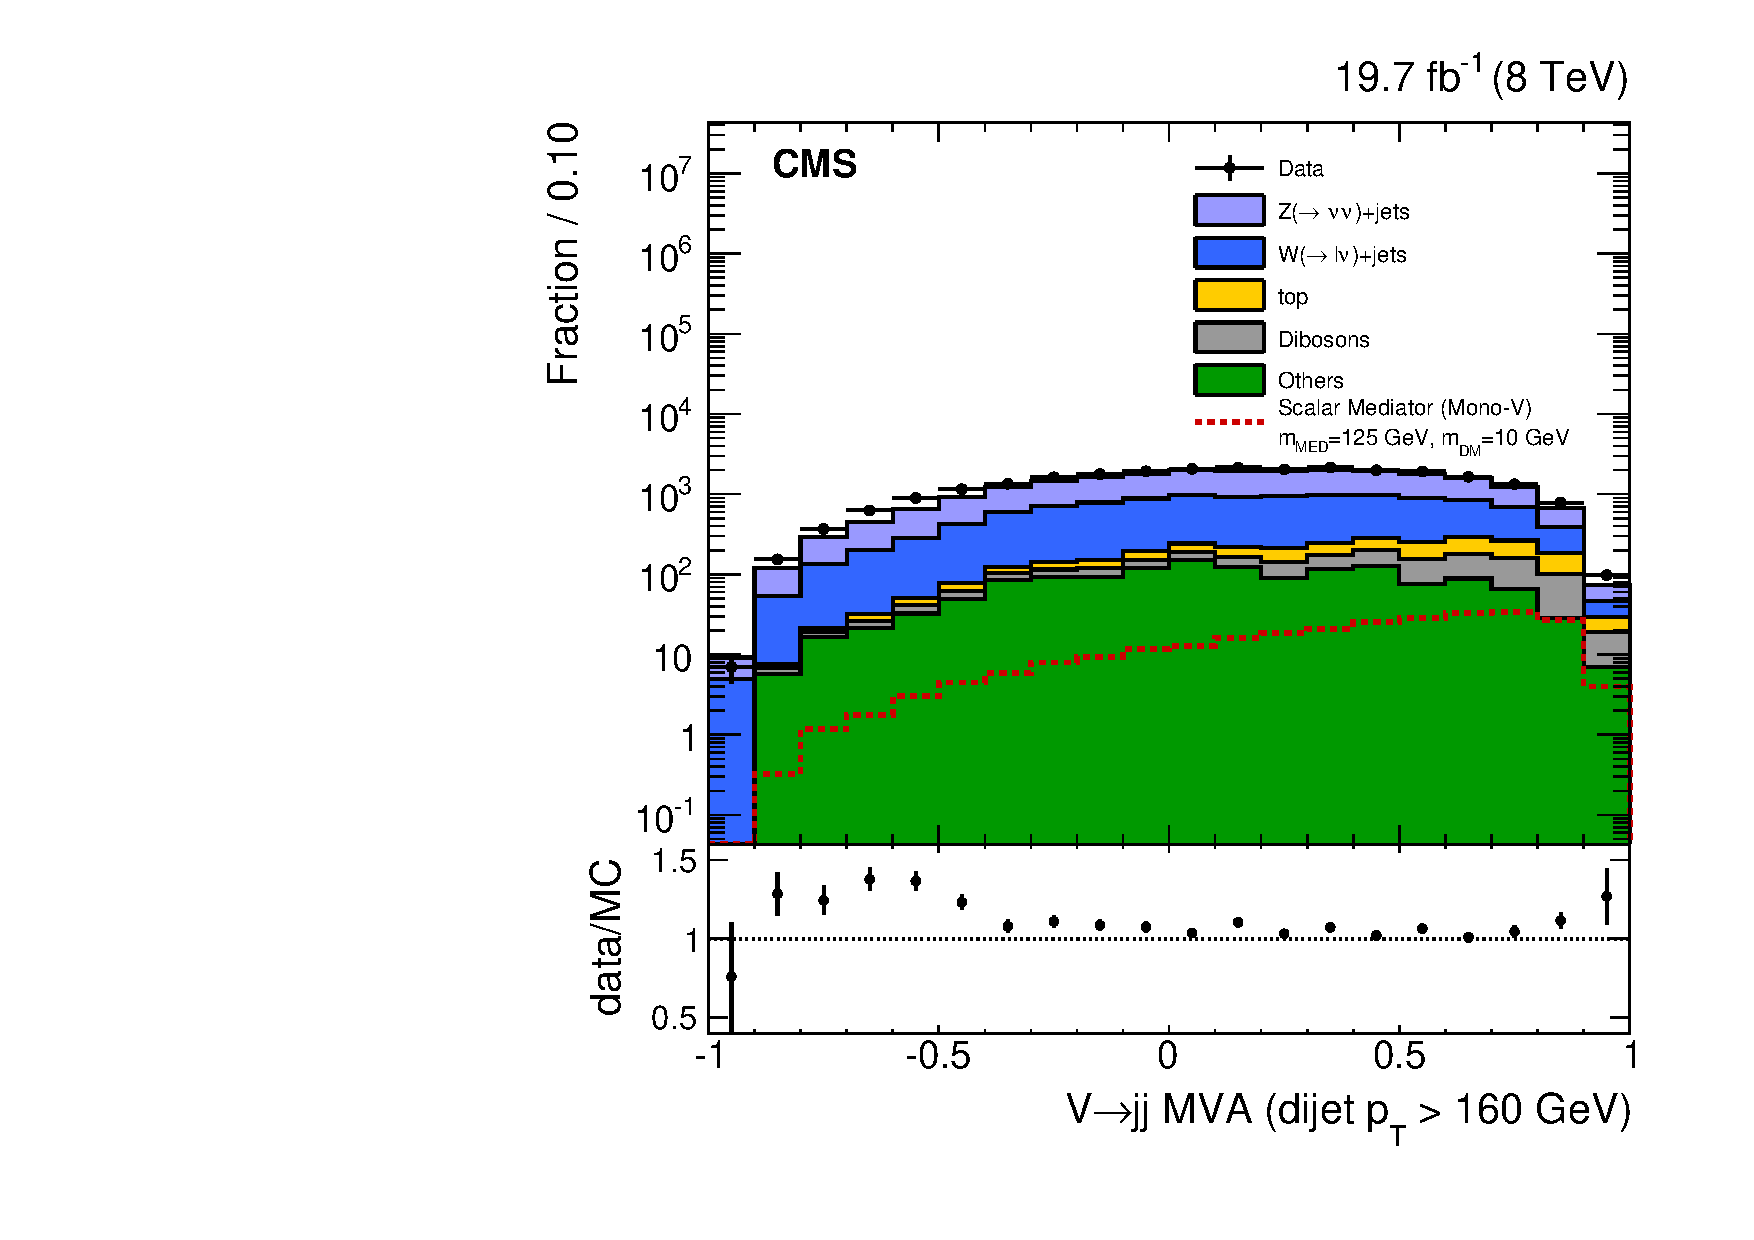
\includegraphics[width=0.49\textwidth]{figures/res_vmvalog_1.pdf}
}
 \caption{
Resolved V-tagger variable distribution in simulation and data after all other
signal region cuts in the resolved category. 
The distributions are shown split into dijet $\pt < 160$ \gev (a) and dijet
$\pt > 160$ \gev (b), corresponding roughly to the point at which jets begin to overlap. 
The expected distribution for the vector boson produced in association with a scalar mediator with is shown.} 
 \label{fig:vtagger}\end{center}\end{figure*}

To reduce contamination from top backgrounds, the event is rejected if it contains a 
b-tagged jet, defined using the CSV medium definition~\cite{BTAG}. Finally, the events are required to 
have $\ETm>250$ \gev. 

The events that do not qualify for either of the two V-tagged categories are required to have a one or two high \pt jets showing characteristics indicative of originating from a \emph{single} quark or gluon. 
For the monojet category, at least one ak5 jet within $|\eta|<2.0$ with \pt greater 
than 150 \gev and a \ETm greater than 200 \gev is required.  
As in the boosted category, events with a second ak5 jet close to the leading one ($\Delta\phi(j_1,j_2) < 2$) 
with $p_T>30$ GeV and $|\eta|<2.5$ are selected to allow the frequent cases where initial state radiation yields two jets.
Events with three or more ak5 jets with $p_T>30$ \gev and $|\eta|<2.5$ are rejected.

To model the expectation from SM backgrounds, simulated samples are produced for the
Z+jets, W+jets, $t\bar{t}$, single-top, and QCD multi-jet processes
using Madgraph~\cite{amcatnlo} interfaced with Pythia6~\cite{Sjostrand:2006za} for hadronization and
fragmentation, where jets from the matrix element are matched to the parton shower following the MLM matching prescription~\cite{Mangano:2006rw}.
Additionally a single-top background sample, produced with
POWHEG~\cite{powheg},  a set of diboson samples, produced directly
with Pythia6, are added. 
The MC samples are corrected to account for the distribution of the number of additional (pileup or PU) interactions
observed in 2012 dataset. Both signal and background samples are additionally corrected to account for the mis-modelling of hadronic recoil in simulation following
the procedure described in~\cite{CMS-PAS-JME-12-002}.


Figure~\ref{fig:ptandmet} shows the \ETm and leading jet $p_{T}$ distributions in data and 
simulation after selection for all three event classes combined. The backgrounds are normalized to 19.7\fbinv 
and the expected distribution for vector mediated DM production assuming a DM mass of 10~\GeV and mediator mass of 1~\TeV is shown. 
The discrepancy between the data and simulation is a result of both mis-modelling of the 
detector resolution and an imperfect theoretical description of the kinematics of the W/Z+jet processes. 
Both effects are corrected for in this analysis using a data-driven approach described in the following section. 

\begin{figure*}[hbtp]\begin{center}
  \subfloat[][]{
 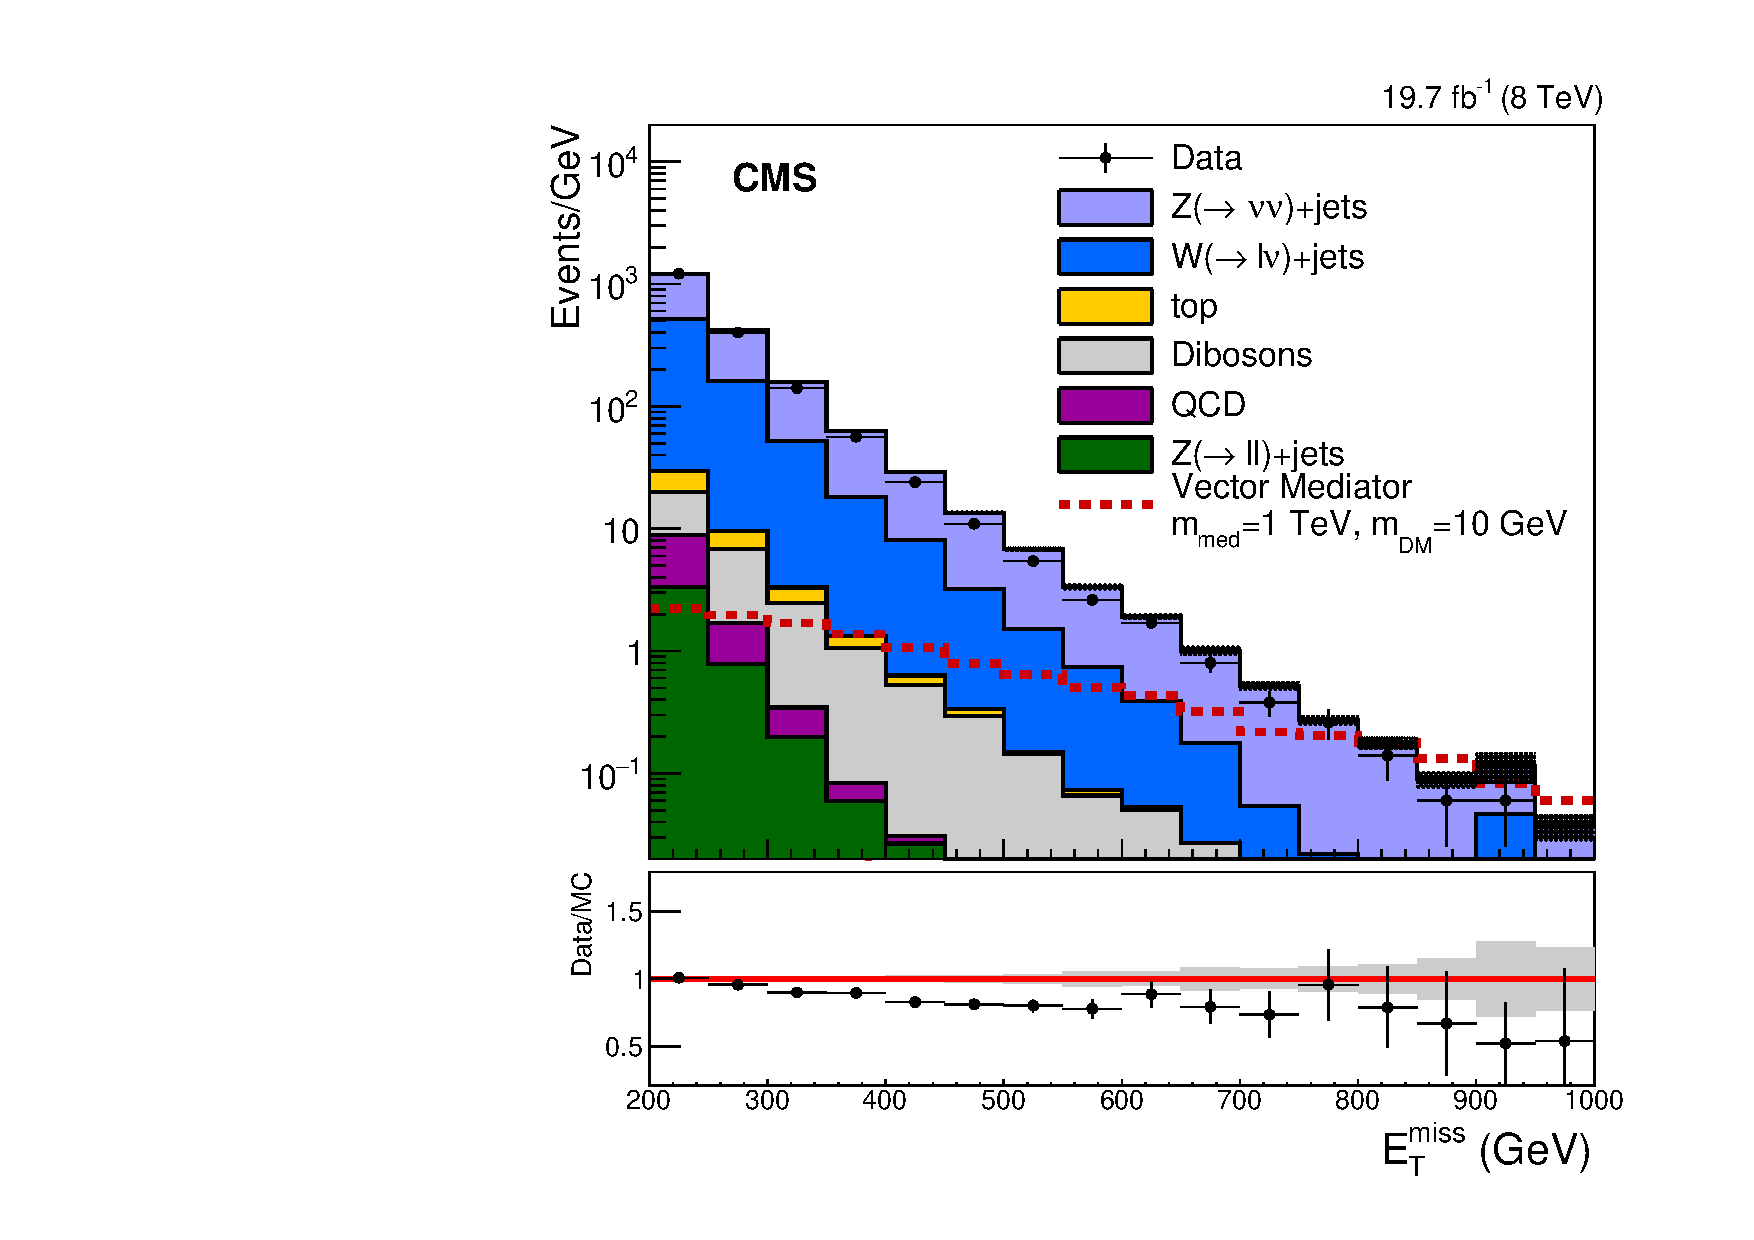
\includegraphics[width=0.49\textwidth]{figures/plot_config_combined_nocorr.pdf}
}
  \subfloat[][]{
 \includegraphics[width=0.49\textwidth]{figures/plot_config_combined_nocorr_jetPT.pdf}\\
}
 \caption{
   Distributions of \ETm (a) and leading jet $p_{T}$ (b) in simulated events and data after the signal selection for all three
   event categories combined. The dashed red line shows the expected distribution assuming vector mediated DM production with $m_{DM}=10$ GeV and $m_{MED}=1$ TeV.
   The gray band in the ratio panels indicate the statistical uncertainty from the limited number of background MC events.
 }
 \label{fig:ptandmet}\end{center}\end{figure*}



\section{Signal Extraction}

The presence of DM production will be observable as an excess of events with respect to the expectations for the 
SM backgrounds in a region at high missing transverse momentum. Significant improvements in terms of sensitivity can be expected if 
several bins in $\ETm$ are considered simultaneously. Further
improvement can be derived by adding control regions, regions orthogonal to
signal with small amounts of signal them, to simultaneously
constrain the predictions of the standard model background. A binned likelihood fit is performed in the range 250 \gev to 1000 \gev (or 200 \gev to 1000 \gev 
for the monojet category), where the binning is chosen to ensure each
corresponding bin of a set of control regions is populated. The width of the highest $\ETm$ bin allows for ease of comparison to the previous CMS search~\cite{monojet1}. 

Data from three control regions, the dimuon and photon control regions, and the single-muon control region, are used to determine the contributions from \Zvvjets~and 
\Wlvjets~respectively. The events in the control regions are divided into the three  categories, using the same selection criteria as 
described in Section~\ref{sec:selection}. In the dimuon, single-muon and photon control regions, the dimuon pair, single-muon or the photon's 
momentum are removed and the \ETm ~is recalculated yielding a distribution of fake \ETm. The distribution of fake \ETm 
in data in the control regions is used to derive the expectation from the Z+jets and W+jets backgrounds in the signal region.

As the decay branching ratio of \Zmm~is approximately 6 times smaller than that to neutrinos, the resulting statistical 
uncertainty on the \Zvvjets~template becomes a dominant systematic uncertainty at large values of \ETm.
A complementary approach is to use events in data that have a high-$p_{T}$ 
photon recoiling against jets to further constrain the \Zvvjets~background template~\cite{CMS-PAS-SUS-08-002}. This is advantageous since the production cross-section 
of \phojets~is roughly 3 times that of the \Zvvjets~resulting in a smaller statistical uncertainty on the predicted background. 
 
The \ETm spectra of the V+jets backgrounds are determined through the use of a likelihood fit, simultaneously across all bins 
in the three control regions. 
The expected number of events $N_{i}$ in a given bin $i$ of fake \ETm, for a particular event category, is given by, 
$N^{Z_{\mu\mu}|\gamma }_{i}=  \dfrac{{\mu^{\Zvv}_{i}}}{R^{Z|\gamma}_{i}}$, 
for the dimuon and photon control regions and  $N^{W}_{i} =  \dfrac{{\mu^{\Wlv}_{i}}}{R^{W}_{i}}$,
for the single-muon control region. The parameters $\boldsymbol{\mu}^{\Zvv}$ and $\boldsymbol{\mu}^{\Wlv}$ are the free parameters 
of the likelihood representing the yields of $\Zvvjets$ and $\Wlvjets$
in each bin of the signal region. The additional terms  $R^{W}_{i}$,
$R^{Z|\gamma}_{i}$ denote transfer factors which account for the
extrapolation of a sepcific background from the signal region to the control regions. The likelihood function for a 
particular category, $c$, is given as,   

\begin{align*}
\mathcal{L}_{\textrm{c}}(\boldsymbol{\mu}^{\textrm{c},\Zvv},\boldsymbol{\mu}^{\textrm{c},\Wlv},\boldsymbol{\theta},\boldsymbol{\phi}) &=        
                \prod_{i} \mathrm{Poisson}\left(d^{\textrm{c},\gamma}_{i} |B^{\textrm{c},\gamma}_{i}(\boldsymbol{\phi}) +\frac{ \mu^{\textrm{c},\Zvv}_{i} }{R^{\textrm{c},\gamma}_{i}(\boldsymbol{\theta})}   \right) \\
       &~\times \prod_{i} \mathrm{Poisson}\left(d^{\textrm{c},Z}_{i}      |B^{\textrm{c},Z}_{i}(\boldsymbol{\phi})      +\frac{ \mu^{\textrm{c},\Zvv}_{i} }{R^{\textrm{c},Z}_{i}     (\boldsymbol{\theta})}       \right ) \\
       &~\times \prod_{i} \mathrm{Poisson}\left(d^{\textrm{c},W}_{i}      |B^{\textrm{c},W}_{i}(\boldsymbol{\phi})      +\frac{ \mu^{\textrm{c},\Wlv}_{i} }{R^{\textrm{c},W}_{i}     (\boldsymbol{\theta})}       \right), \numberthis\label{eqn:candclh}
\end{align*}

where $d^{c,\gamma/Z/W}_{i}$ are the observed number of events in each bin of the photon, dimuon and single-muon control regions.
The expected contributions from background processes in the dimuon, single-muon and photon control regions are denoted $B^{Z}$, $B^{W}$ and 
$B^{\gamma}$ in equation~\ref{eqn:candclh} respectively.

The transfer factors $R^{Z}_{i}$ account for the ratio of $BR(\Zvv)/BR(\Zmm)$ and 
the muon efficiency times acceptance in the dimuon control region, while 
$R^{\gamma}_{i}$ account for the ratio of differential cross-sections between the Z+jet 
and photon+jet processes and the efficiency times acceptance of the photon selection for 
the photon plus jet control region. The differential boson $p_{T}$ cross-sections of 
photon and Z production are first corrected using NLO k-factors derived by  
comparing their $p_{T}$ distributions in events generated with Madgraph5\_aMC@NLO~\cite{amcatnlo}, and subsequently showered,  
to the distributions produced at leading order before deriving the transfer factors. 

Systematic uncertainties are modelled as constrained nuisance parameters, $\boldsymbol{\theta}$, which allow for variation of 
the transfer factors, $R^{\gamma/Z/W}$, in the fit and are treated as fully correlated between event categories.
These include theoretical uncertainties on the photon to Z differential cross-section ratio from renormalization and factorization scale uncertainties. 
Electroweak corrections to the ratio are not accounted for in the simulation. The full correction is also taken as an uncertainty on the ratio, 
which is of the order of 15\% when the boson (Z or $\gamma$) \pt is at the TeV scale~\cite{Kuhn:2005gv}. A conservative choice is made in assuming 
this uncertainty to be uncorrelated across bins of \ETm. Additionally, the uncertainty in the muon selection efficiency, photon selection efficiency, 
and photon purity are included and fully correlated across the event categories and control regions, where relevant. A systematic uncertainty of 10\% 
is included for the top and diboson background normalizations~\cite{tagkey2015250} and correlated between the single-muon and dimuon control regions. The results of a fit to the control regions are shown in Figure~\ref{fig:combined_fit_result}.
 
\begin{figure*}[hbtp]\begin{center}
 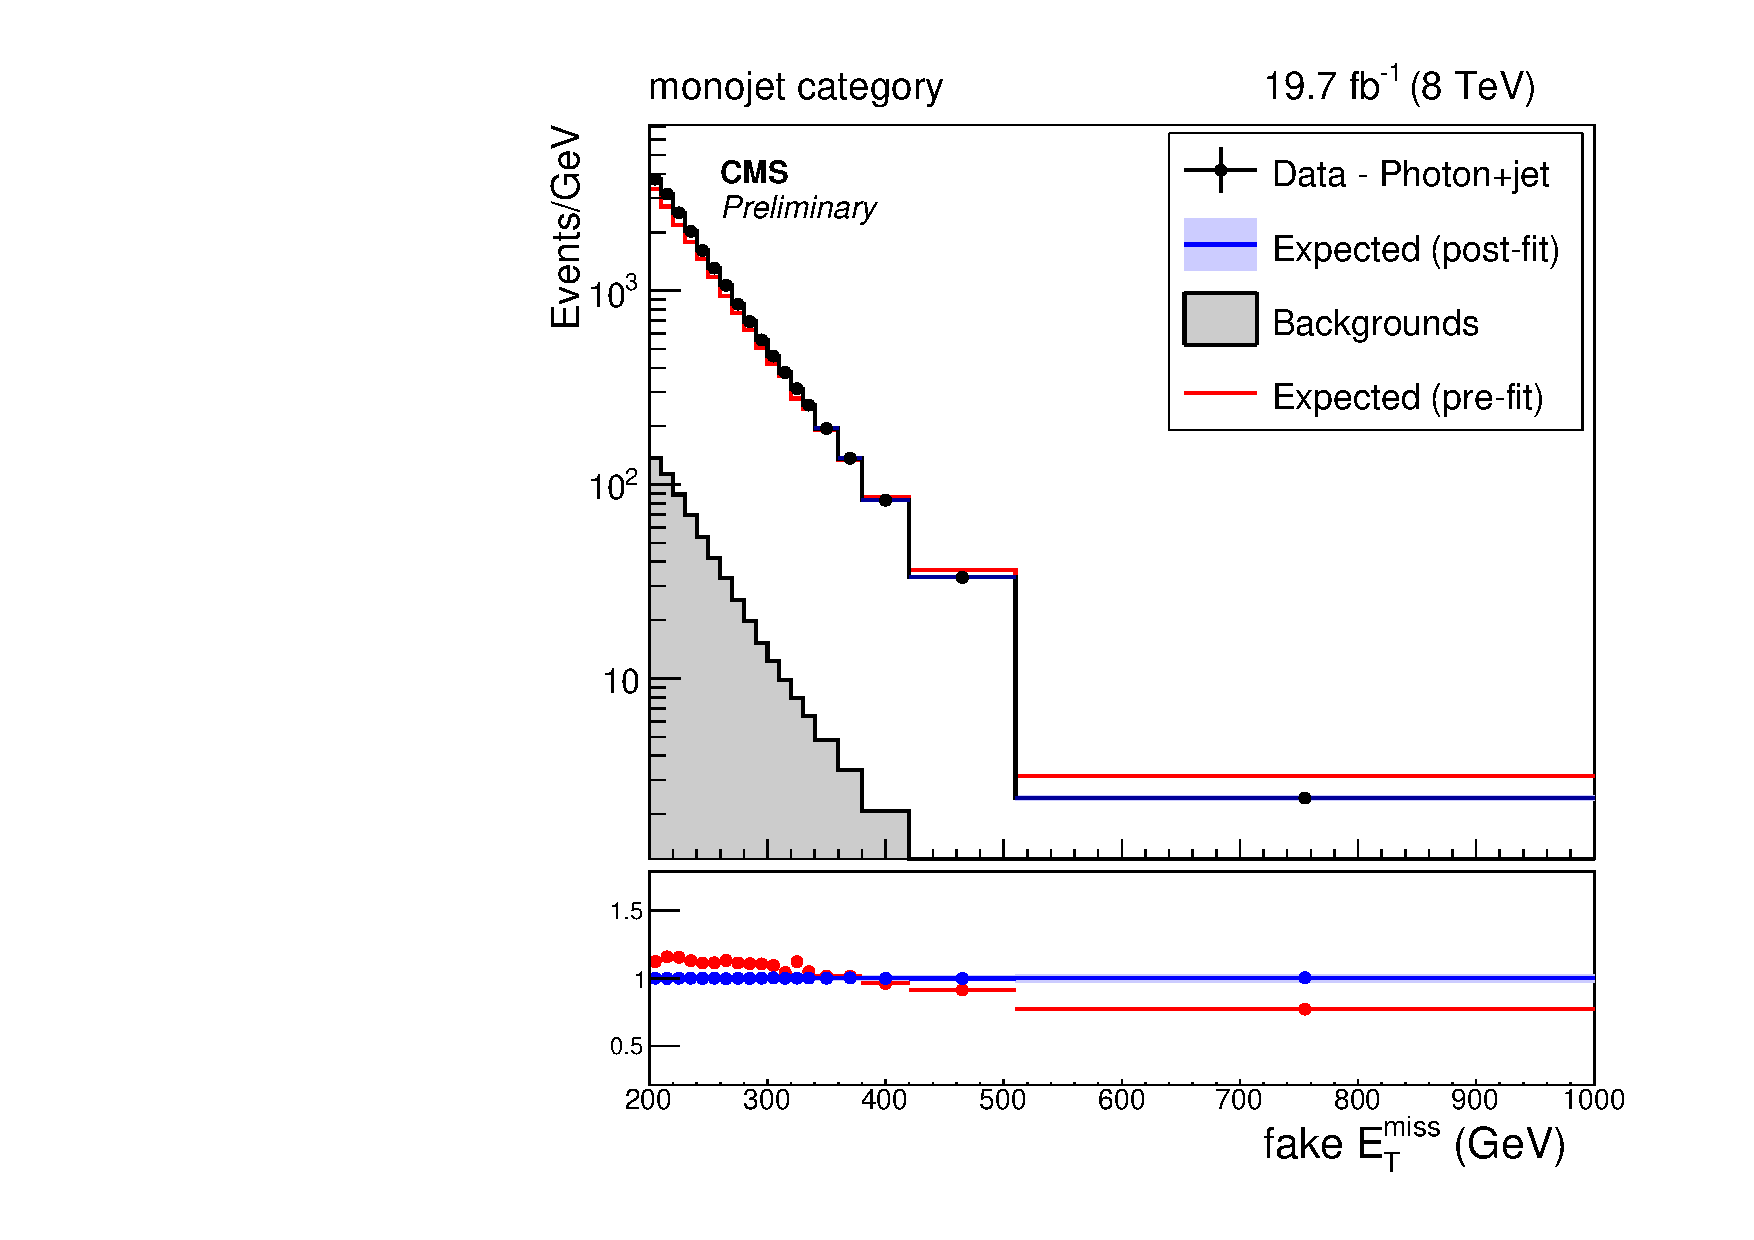
\includegraphics[width=0.32\textwidth]{figures/post_fit_photon_monojet.pdf}
 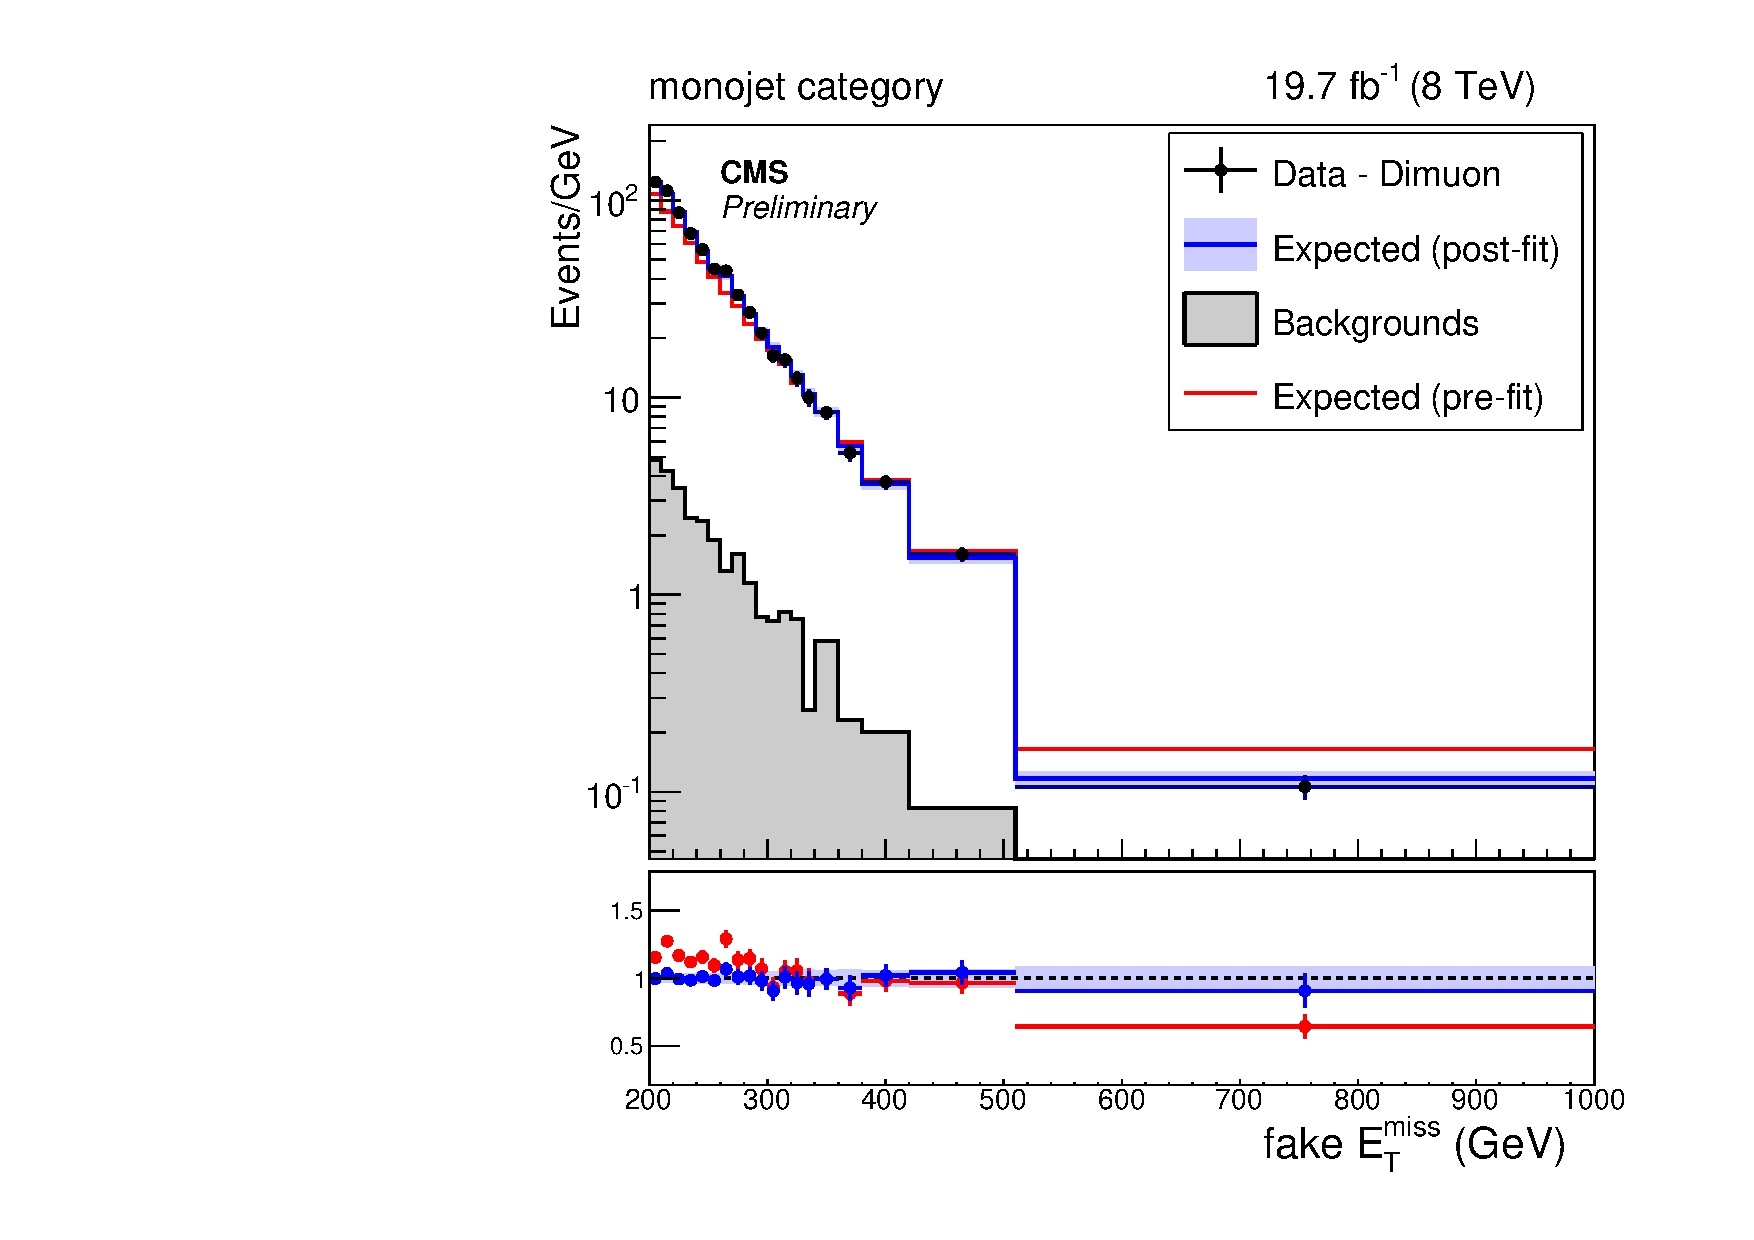
\includegraphics[width=0.32\textwidth]{figures/post_fit_zmm_monojet.pdf}
 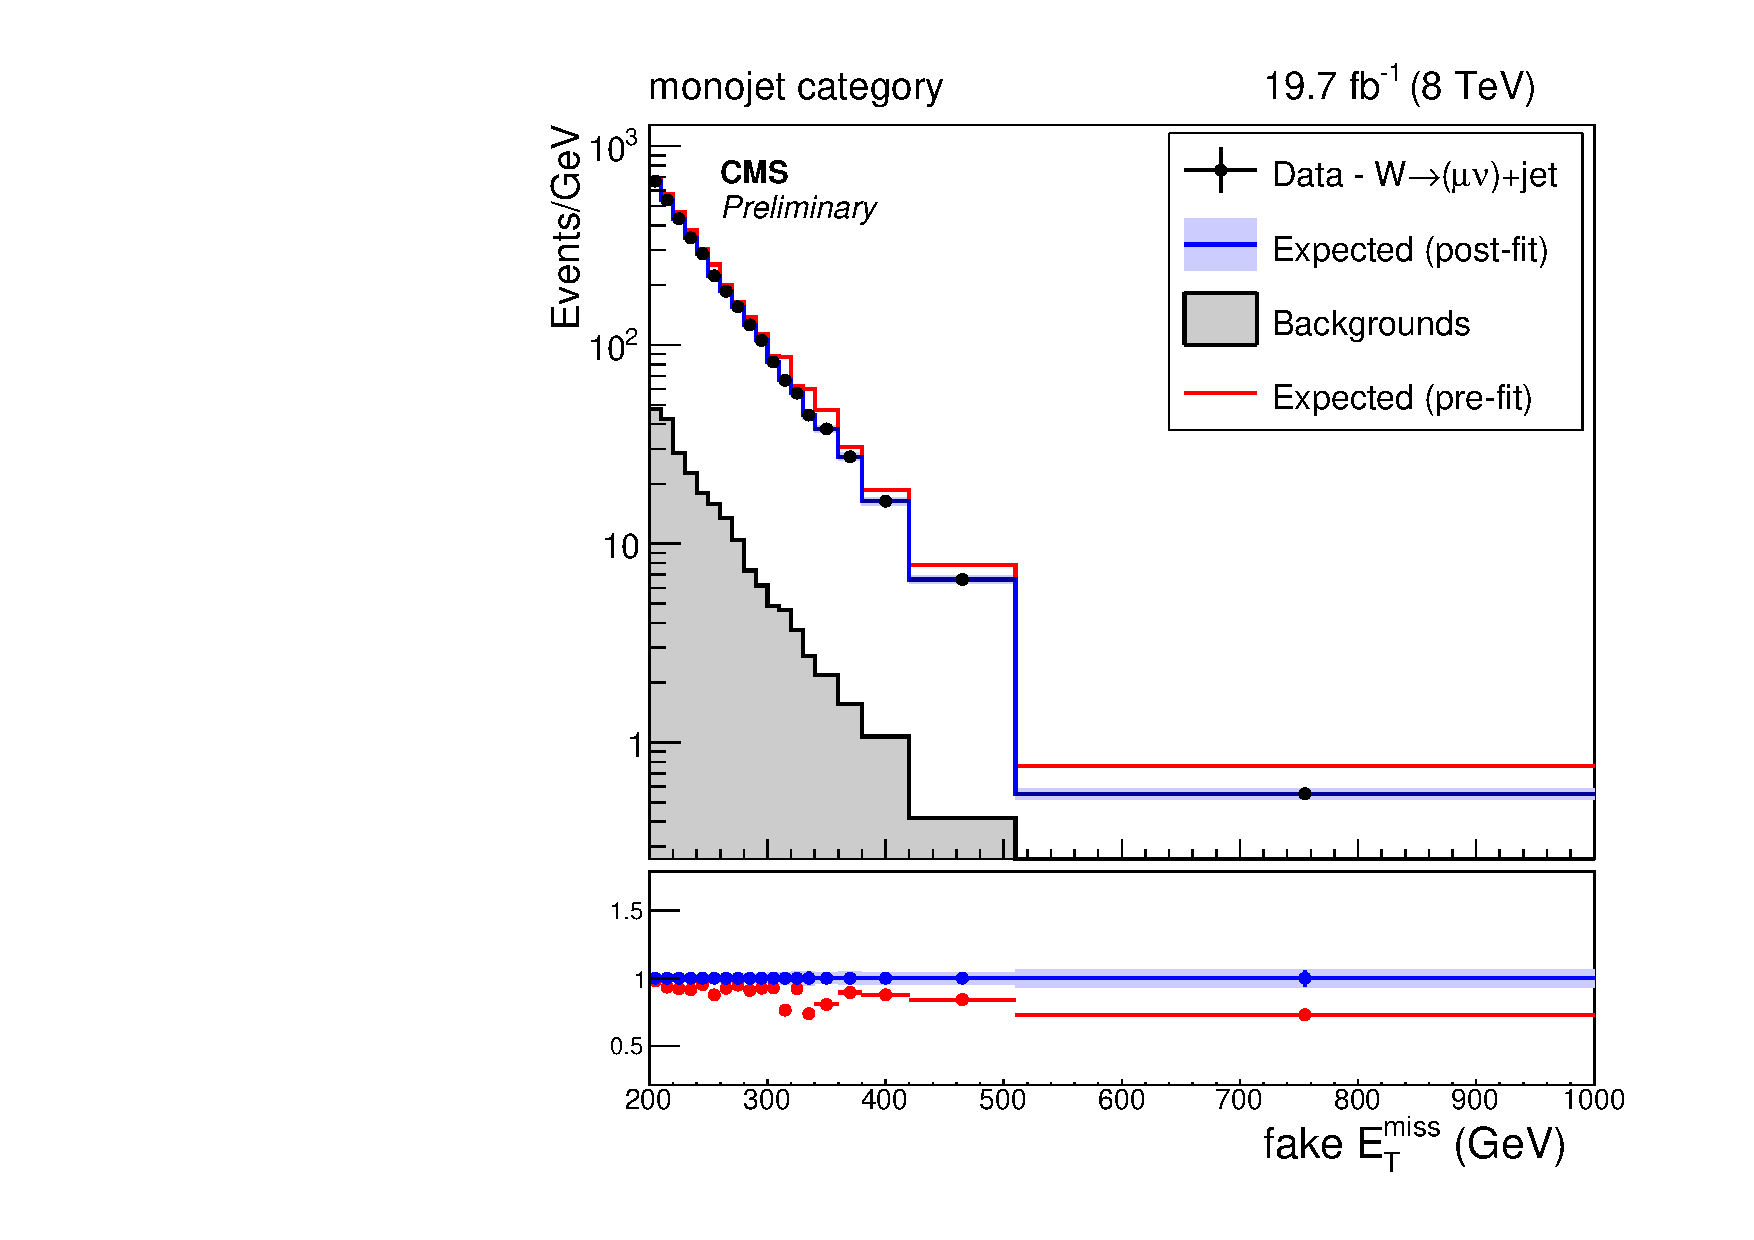
\includegraphics[width=0.32\textwidth]{figures/post_fit_wmn_monojet.pdf}\\
 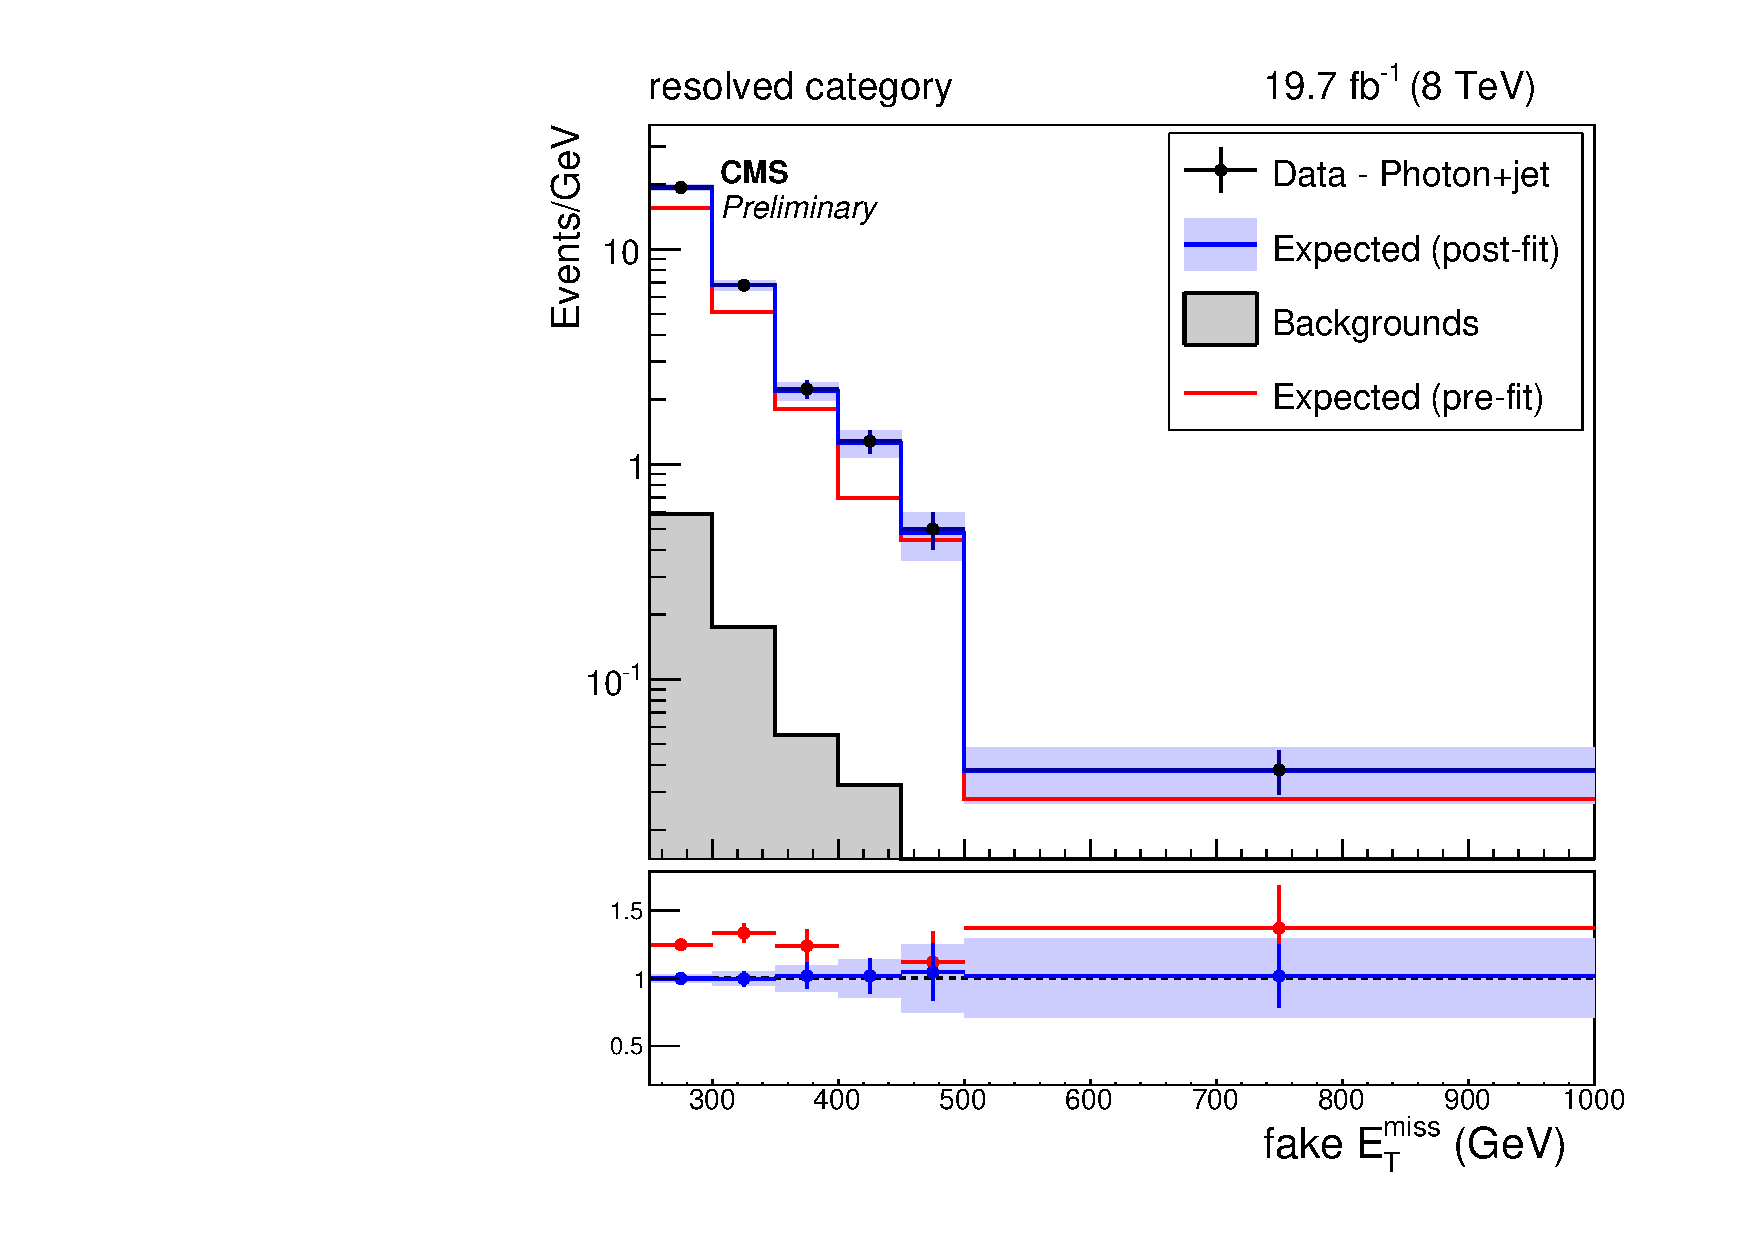
\includegraphics[width=0.32\textwidth]{figures/post_fit_photon_resolved.pdf}
 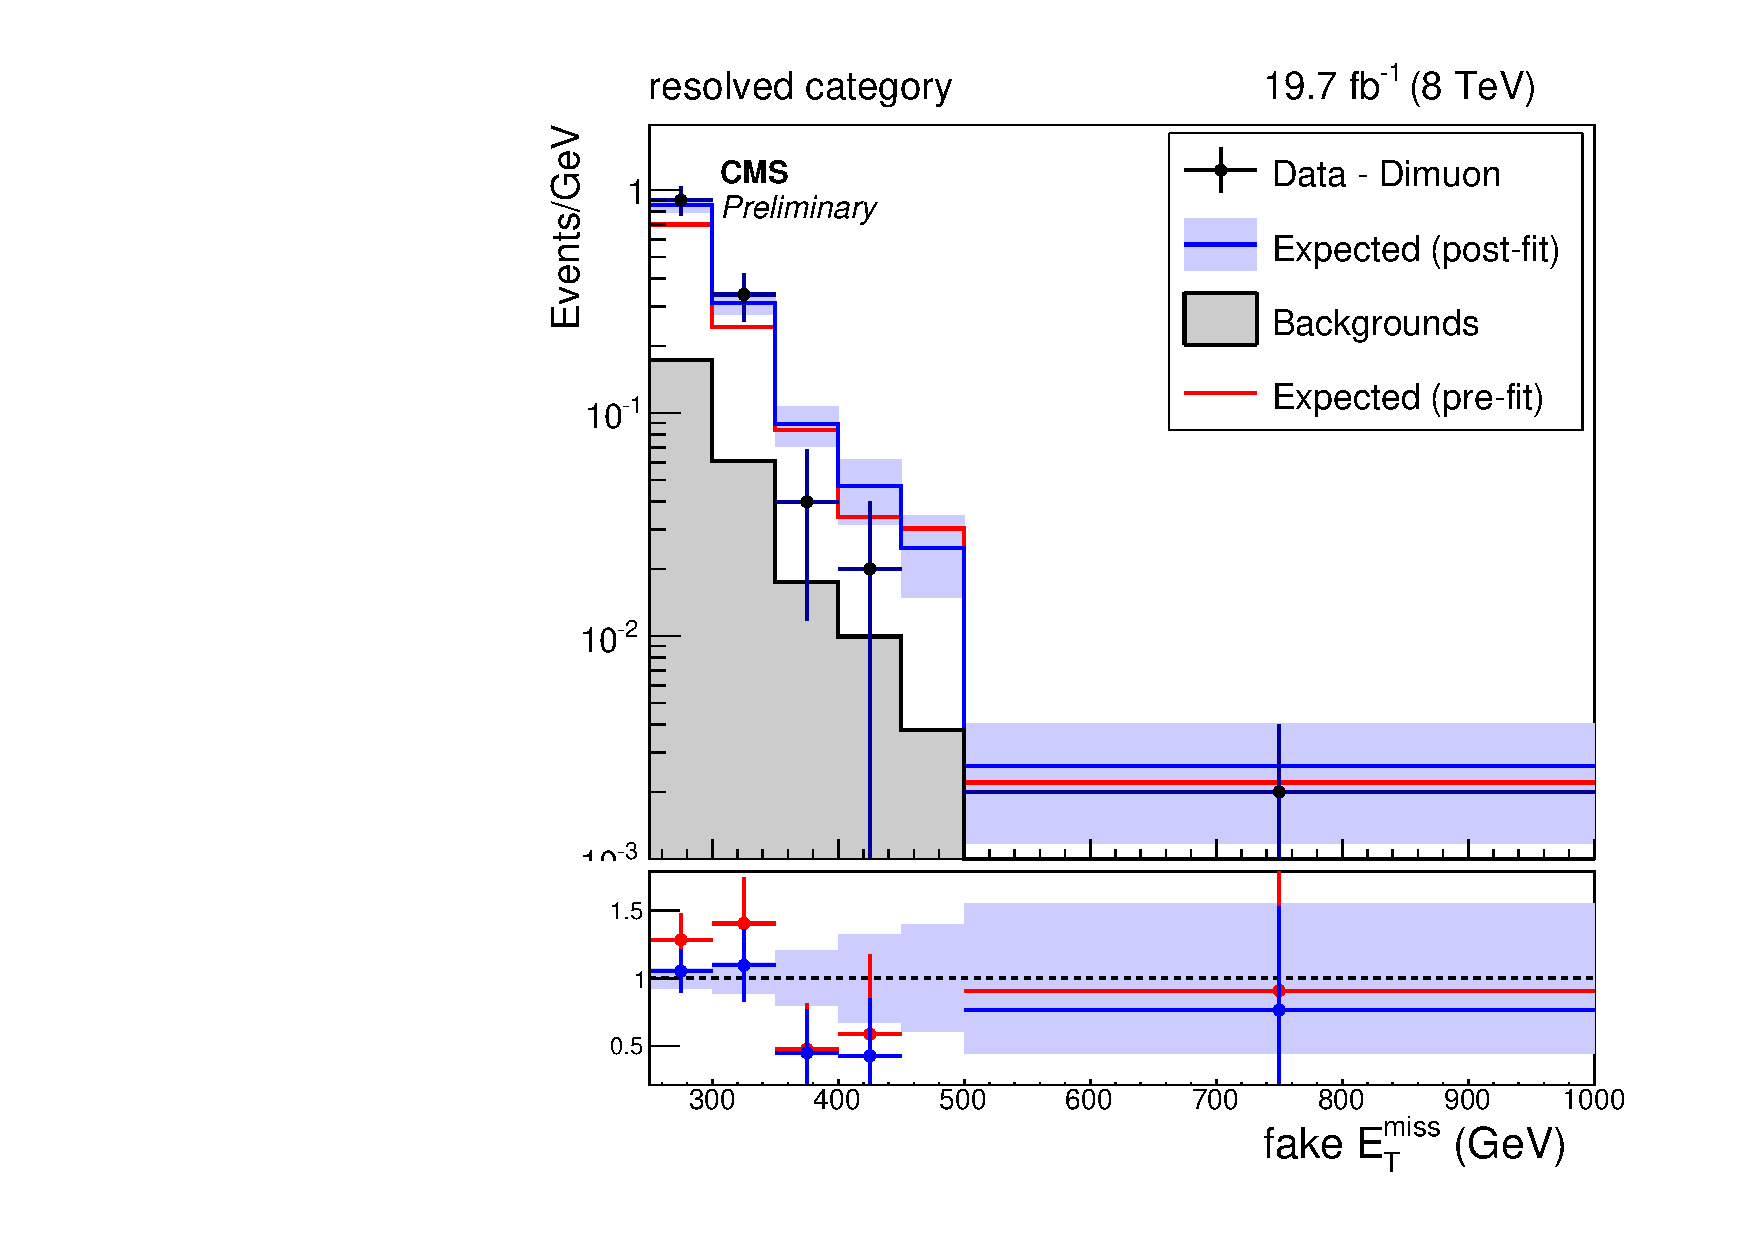
\includegraphics[width=0.32\textwidth]{figures/post_fit_zmm_resolved.pdf}
 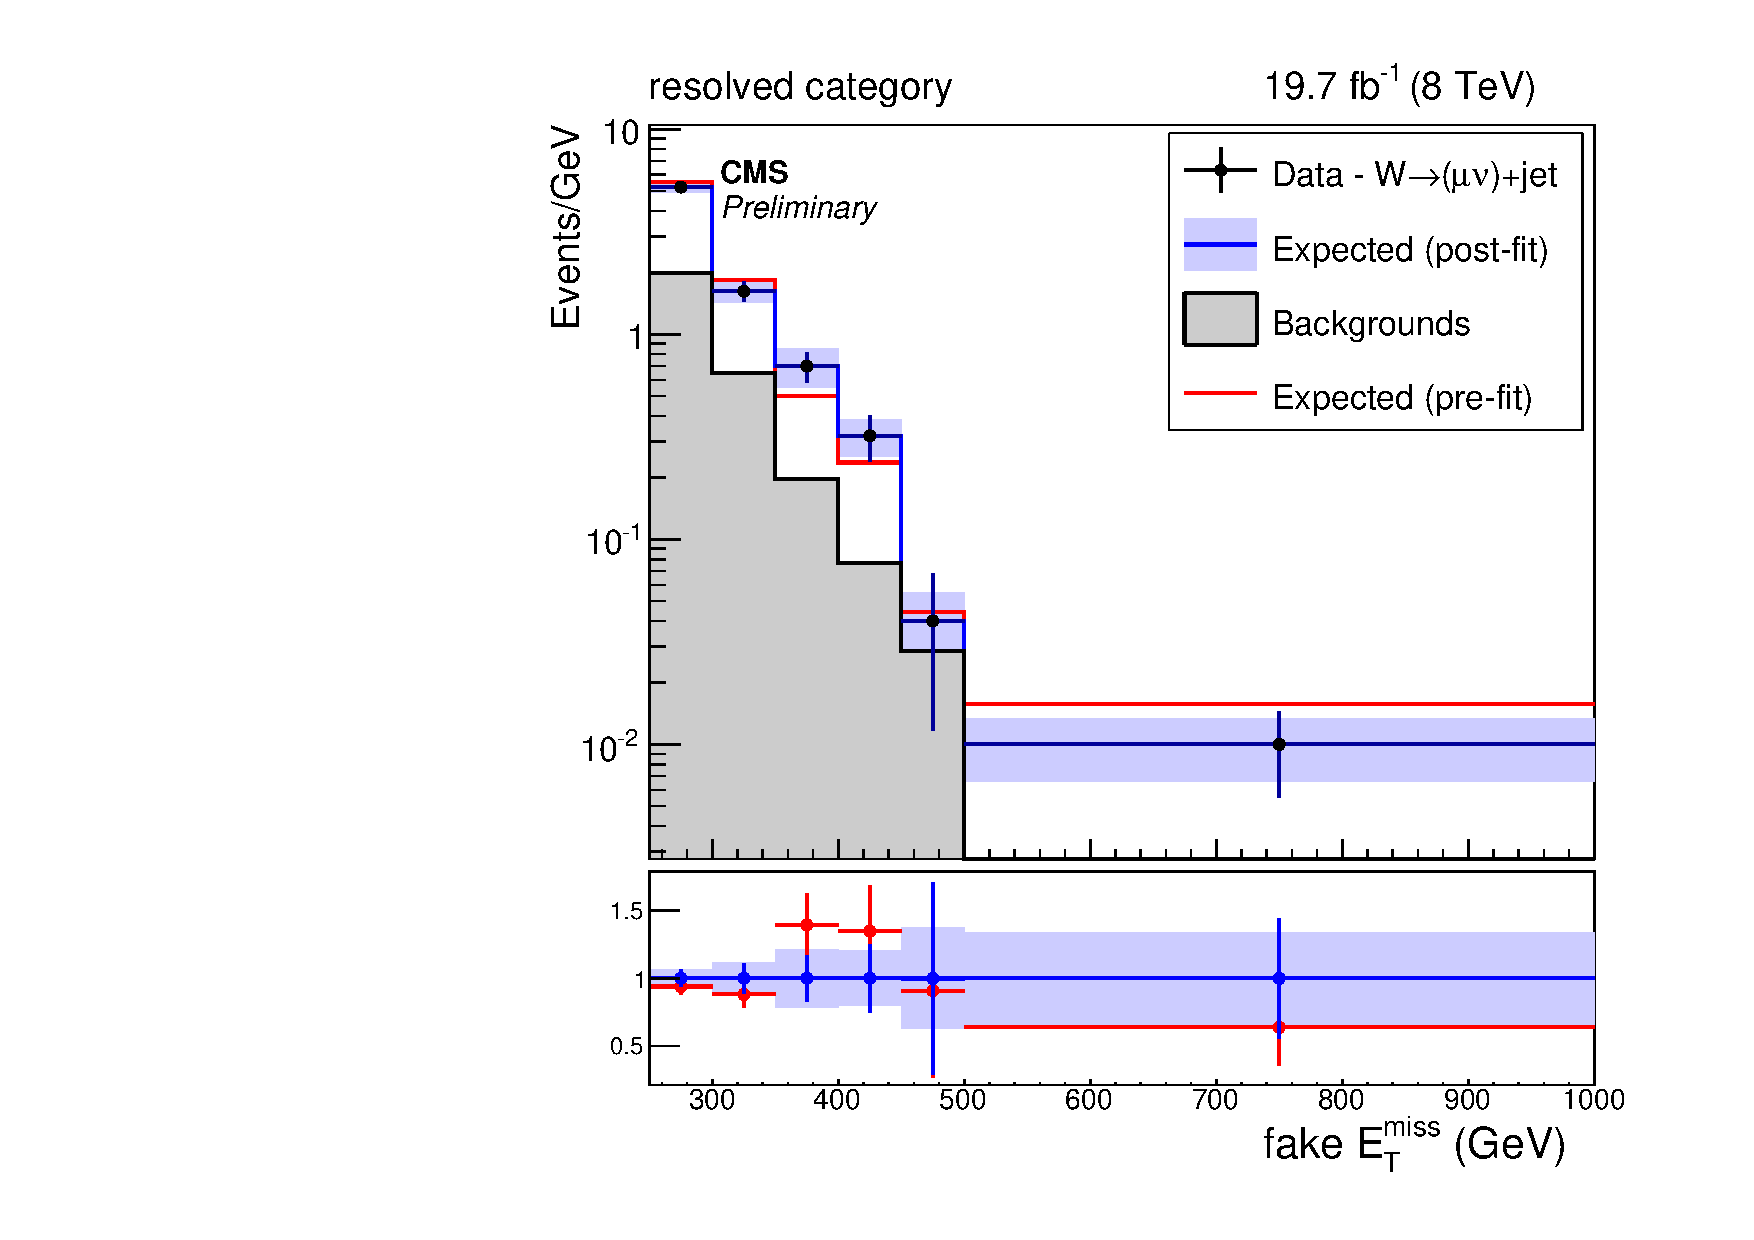
\includegraphics[width=0.32\textwidth]{figures/post_fit_wmn_resolved.pdf}\\
 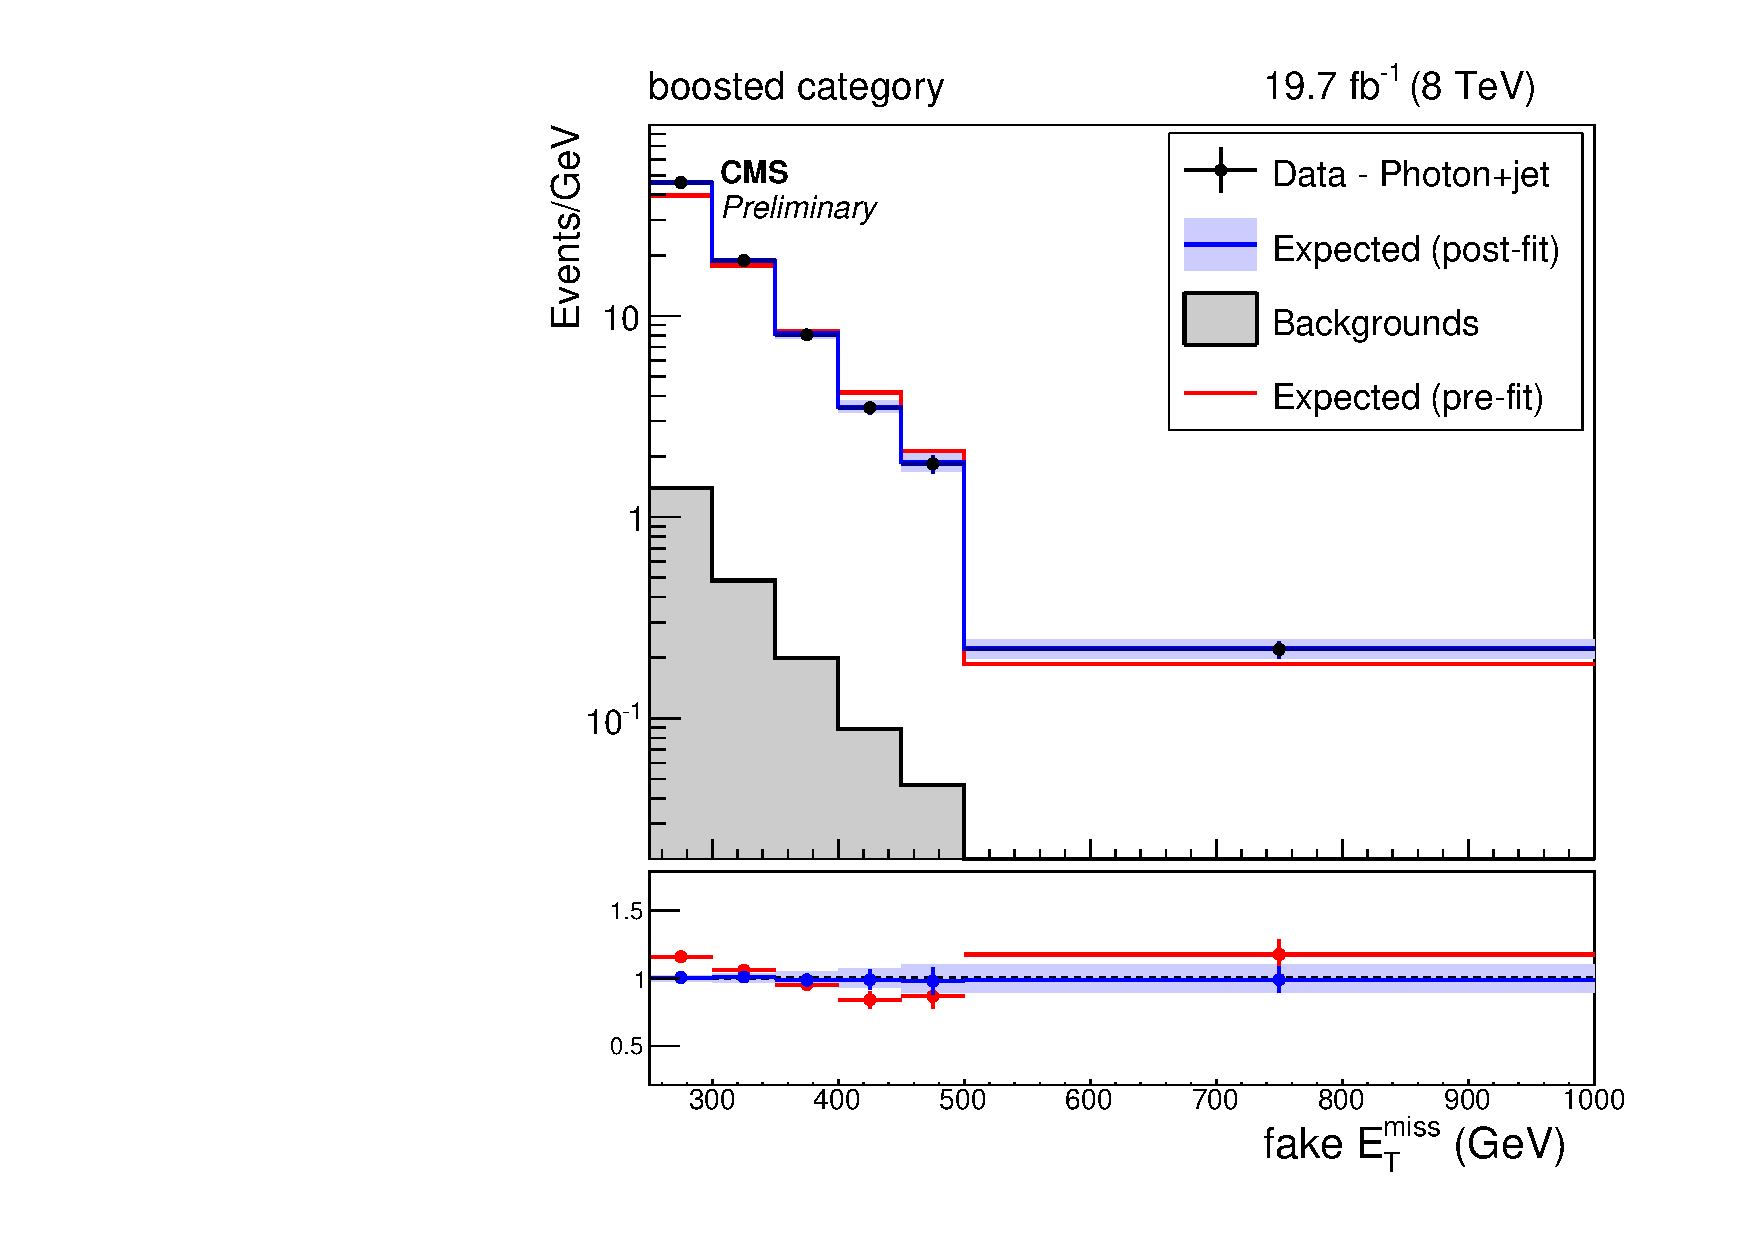
\includegraphics[width=0.32\textwidth]{figures/post_fit_photon_boosted.pdf}
 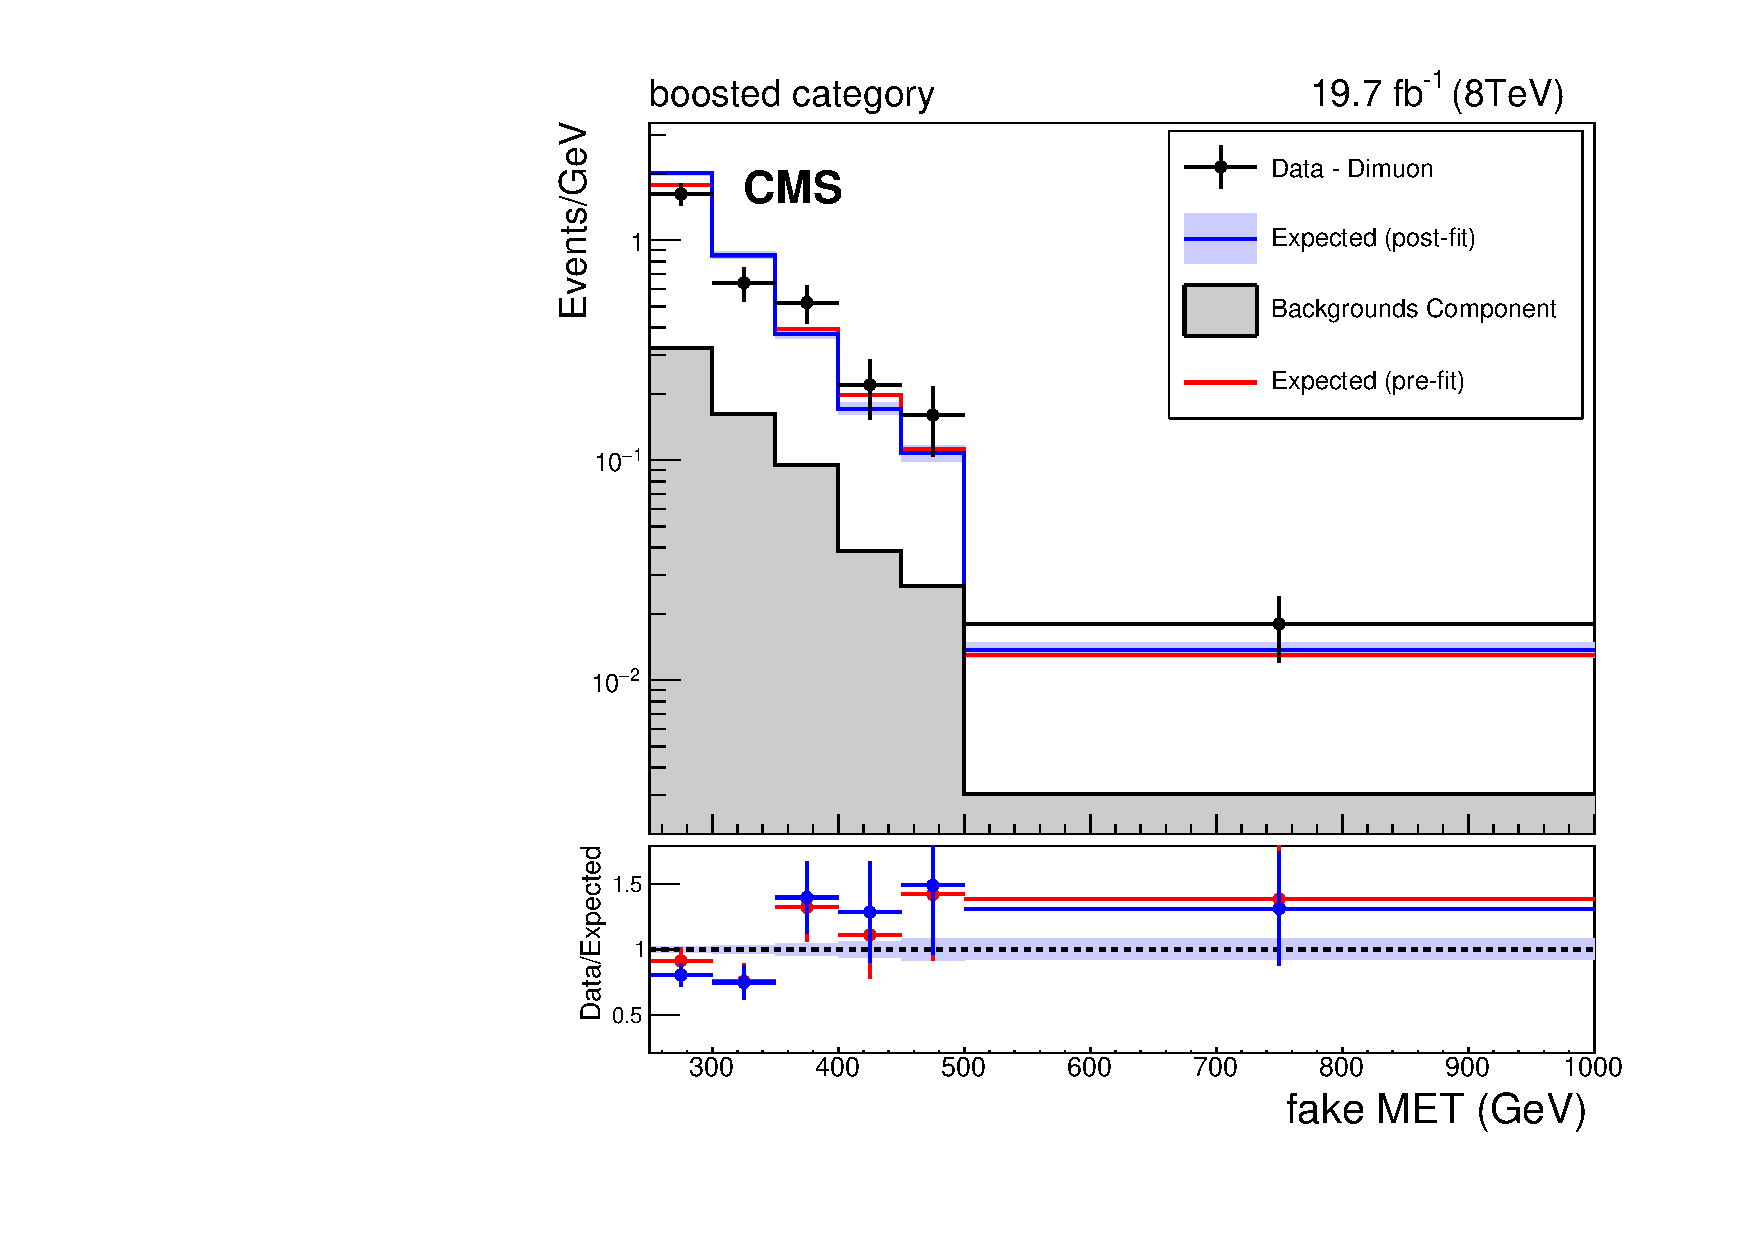
\includegraphics[width=0.32\textwidth]{figures/post_fit_zmm_boosted.pdf}
 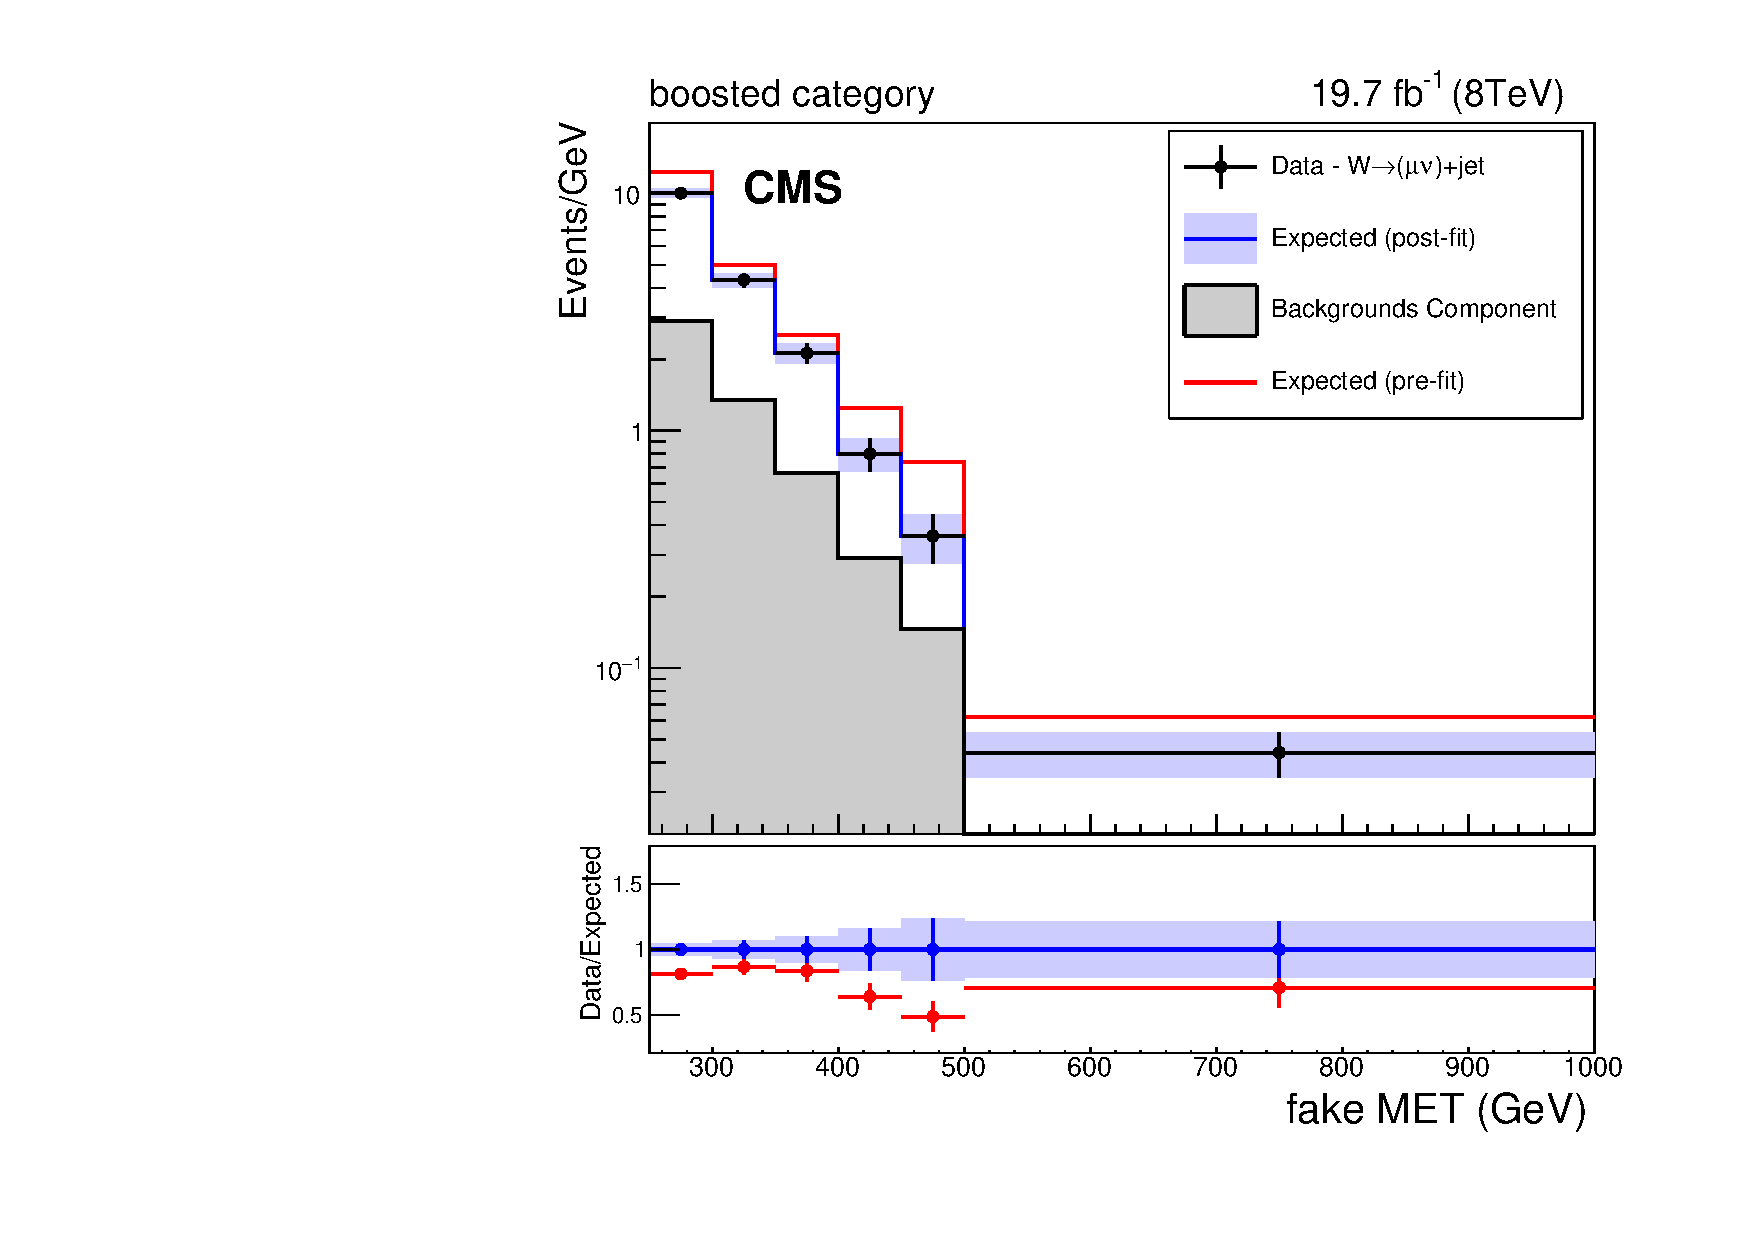
\includegraphics[width=0.32\textwidth]{figures/post_fit_wmn_boosted.pdf}\\
\end{center}
 \caption{Expected and observed fake \ETm distributions in the photon~(\cmsLeft), dimuon (middle) and single-muon~(\cmsRight) 
 control regions after performing the simultaneous likelihood fit to the control regions. 
 Each row, from top to bottom, shows the result of the fit in the monojet, resolved and boosted event categories 
 respectively. The red line represents the expected distribution before fitting to the control regions, while the blue line shows the expectation after 
 the fit. In the ratio, the blue and red points show the ratio of the observed data to the post-fit and pre-fit expectations 
 respectively. The blue bands indicate the statistical and systematic uncertainties from the fit.\label{fig:combined_fit_result} }
\end{figure}

The remaining backgrounds are expected to be much smaller than those from V+jets and are estimated directly from the simulation. 
Shape and normalization systematic uncertainties from the recoil corrections applied to these 
backgrounds are included to account for the uncertainty in the energy scale and resolution 
of jets. Additionally, a systematic uncertainty of 4\% is included for the top backgrounds due to the uncertainty of 
the b-tagging efficiency for the b-jet veto in the resolved category. Systematic uncertainties of 7\%, 10\% and 50\% are included for the top~\cite{Khachatryan:2015oqa}, diboson~\cite{tagkey2015250,Khachatryan:2015sga} and QCD backgrounds~\cite{Khachatryan:2014rra} respectively to account for the uncertainty in their production cross-sections. These individual backgrounds have been studied separately using dedicated control regions in data in order to validate these systematic uncertainties. Finally, a systematic uncertainty of 2.6\% in the luminosity 
measurement~\cite{lumi} is included for all of the MC derived backgrounds.


%Table~\ref{tab:systematics} gives a summary of the systematic uncertainties on the backgrounds estimation which are propagated to the calculation of the limits.
%Experimental uncertainties in the signal resulting from jet energy scale and resolution and V-tagging efficiency are included in the signal model for all of the interpretations described.

%\begin{table*}[htbp]
%  \begin{center}
%    \topcaption{Systematic uncertainties and their relative effect on the expectation for the SM backgrounds. 
%      \label{tab:systematics}}
%    %\small
%    \begin{tabular}{llccc}
%      \hline
%      \hline
%      Systematic Uncertainty 	   	            & Process & Boosted & Resolved & Monojet  \\
%      \hline
%      \hline
%      Control region fits$^{\dagger}$ & $\Zvvjets$  &6-20\%  &7.6-44\%  &2.5-9.5\%  \\
%      			   	      & $\Wlvjets$  &10.5-55\% &14.5-320\%  &3.6-17\%  \\
%      \hline
%      Tau-id efficiency		& $\Wlvjets$      & 3.6\% & 3.6\% & 3.6\% \\
%      \hline
%      V-tag efficiency$^{\ddagger}$ 		& Dibosons, Top & \multicolumn{2}{c}{10\%,6\% } &  \\ 
%      \hline
%      b-tag efficiency 		& Top & \multicolumn{3}{c}{4\% } \\ 
%      \hline
%      \ETm recoil 		& Dibosons      & 0.6\% & 2.8\% & 0.3\%  \\ 
%       				& Top    	& 1.1\% & 1.8\% & 1.3\%  \\ 
%       				& $\Zlljets$    & 5.8\% & 9.4\% & 0.7\%  \\ 
%      \hline
%      $t\bar{t}$ norm  		& Top 	      & 7\%  & 7\%  & 7\% \\ 
%      Dibosons norm 		& Dibosons    & 10\% & 10\% & 10\%\\ 
%      QCD norm		 	& QCD 	      & 50\% & 50\% & 50\%\\ 
%      \hline
%      Luminosity  	 	& All except V+jets  & 2.6\% & 2.6\% & 2.6\% \\ 
%      \hline 
%      \hline
%    \end{tabular}\\
%    \end{center}
%    \bottomcaption{\footnotesize{$^{\dagger}$ The relevant components of the fit uncertainties relating to theory and muon/photon identification scale-factors 
%	in the control regions, described in Section~\ref{sec:zjetsmodel}, are included here and correlated between event categories.
%	The numbers here indicate the range of the size of the uncertainties (the smallest to largest) in any \ETm bin due to these fits but should not be 
%	interpreted as the systematic uncertainty which is propagated to the signal extraction.
%	For the boosted category, the uncertainty of 320\% is simply the result of a small fitted yield in one of the bins of the single muon control region.\\
%	$^{\ddagger}$ Uncertainty modeled as migration between the V-tagged (boosted and resolved) and monojet categories.
%    }}
%\end{table*}


\begin{section}{Results}

A simultaneous fit to the signal region across the three event categories, allowing for sytematic uncertainty variations of the background expectations, is performed.
The corresponding comparisons between data and background in the \ETm distributions, for each of the three categories, after this fit are shown in Figure~\ref{fig:post_fit_plots}.   
Agreement between the expected SM backgrounds and data is observed at the percent level across the three categories. The largest single-bin local significance across the three categories, is 1.9$\sigma$ and corresponds to the excess seen in the last \ETm bin of the monojet category.

\begin{figure*}[hbtp]\begin{center}
  \subfloat[][]{
 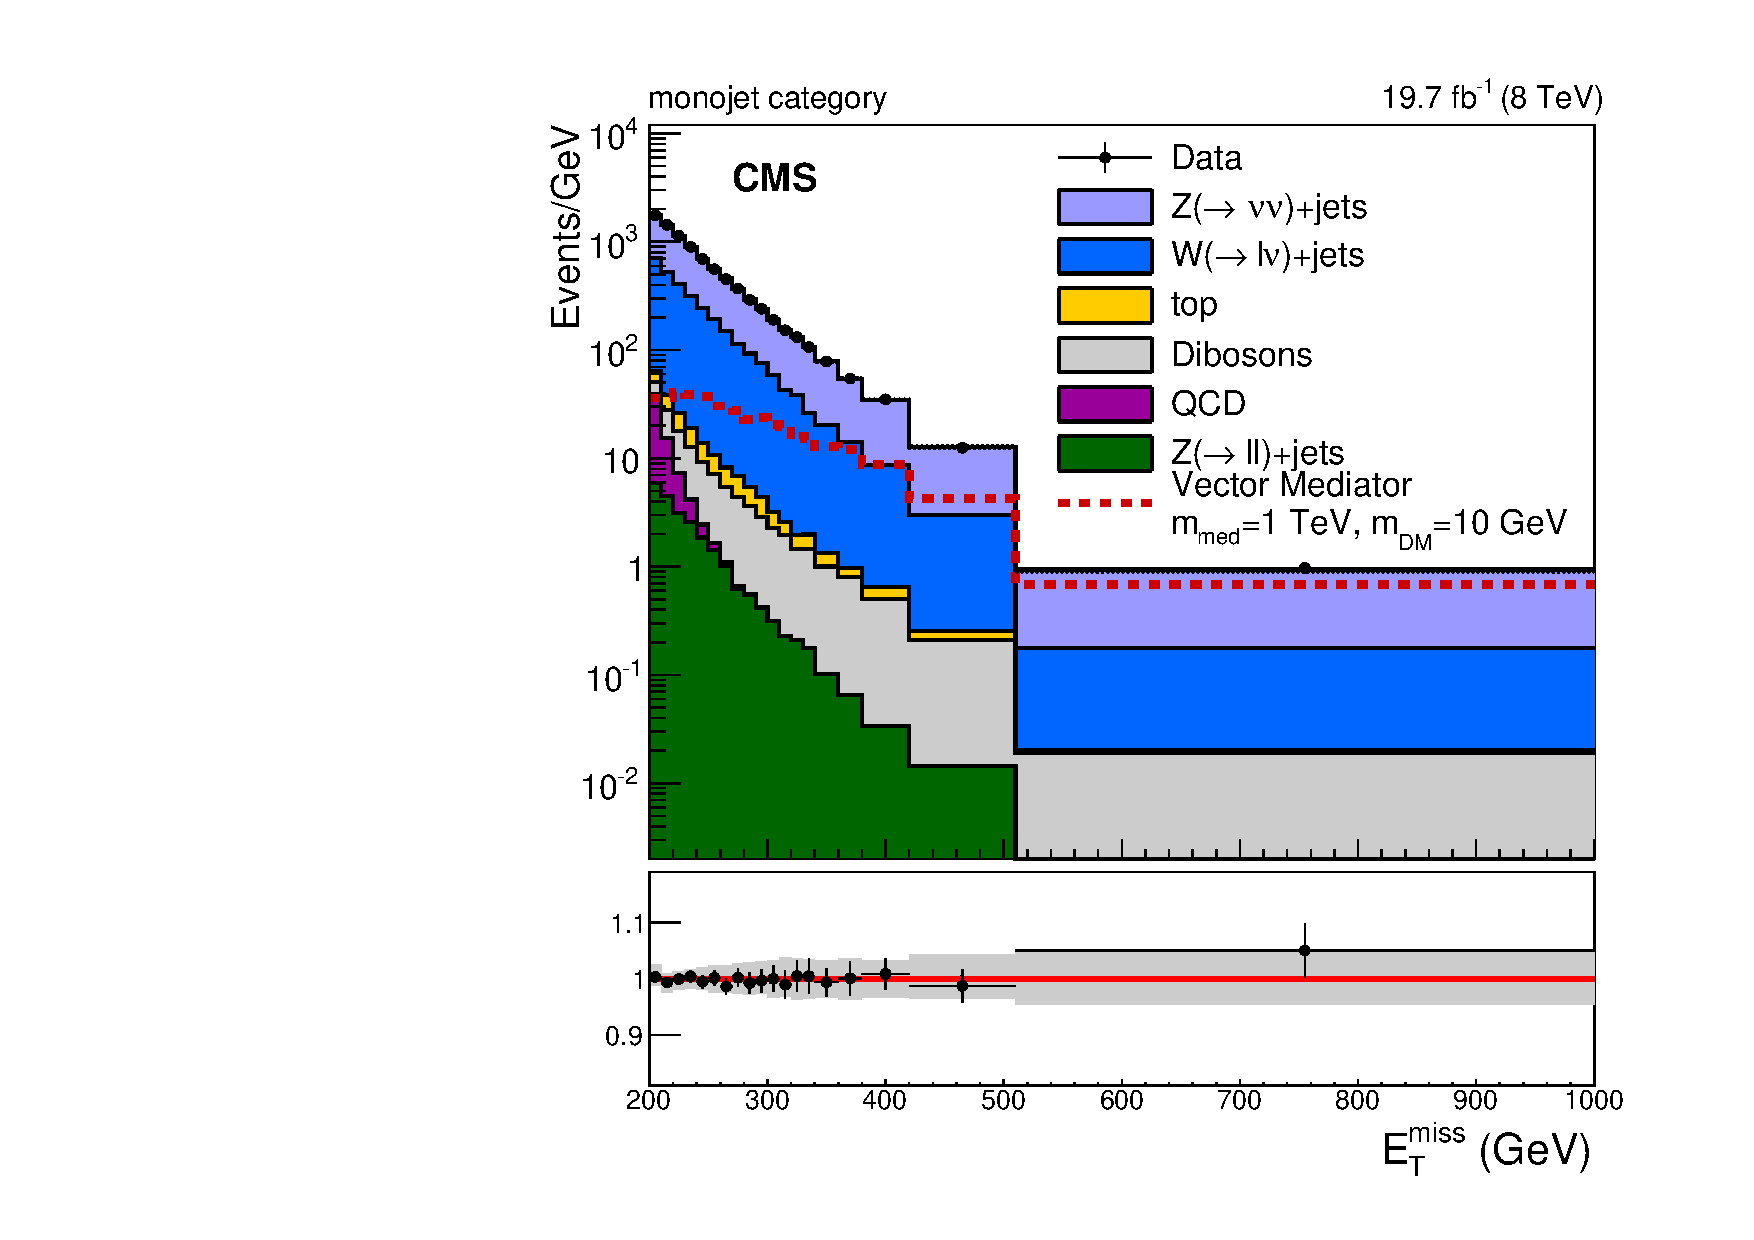
\includegraphics[width=0.5\textwidth]{figures/plot_config_monojet.pdf}
}
  \subfloat[][]{
 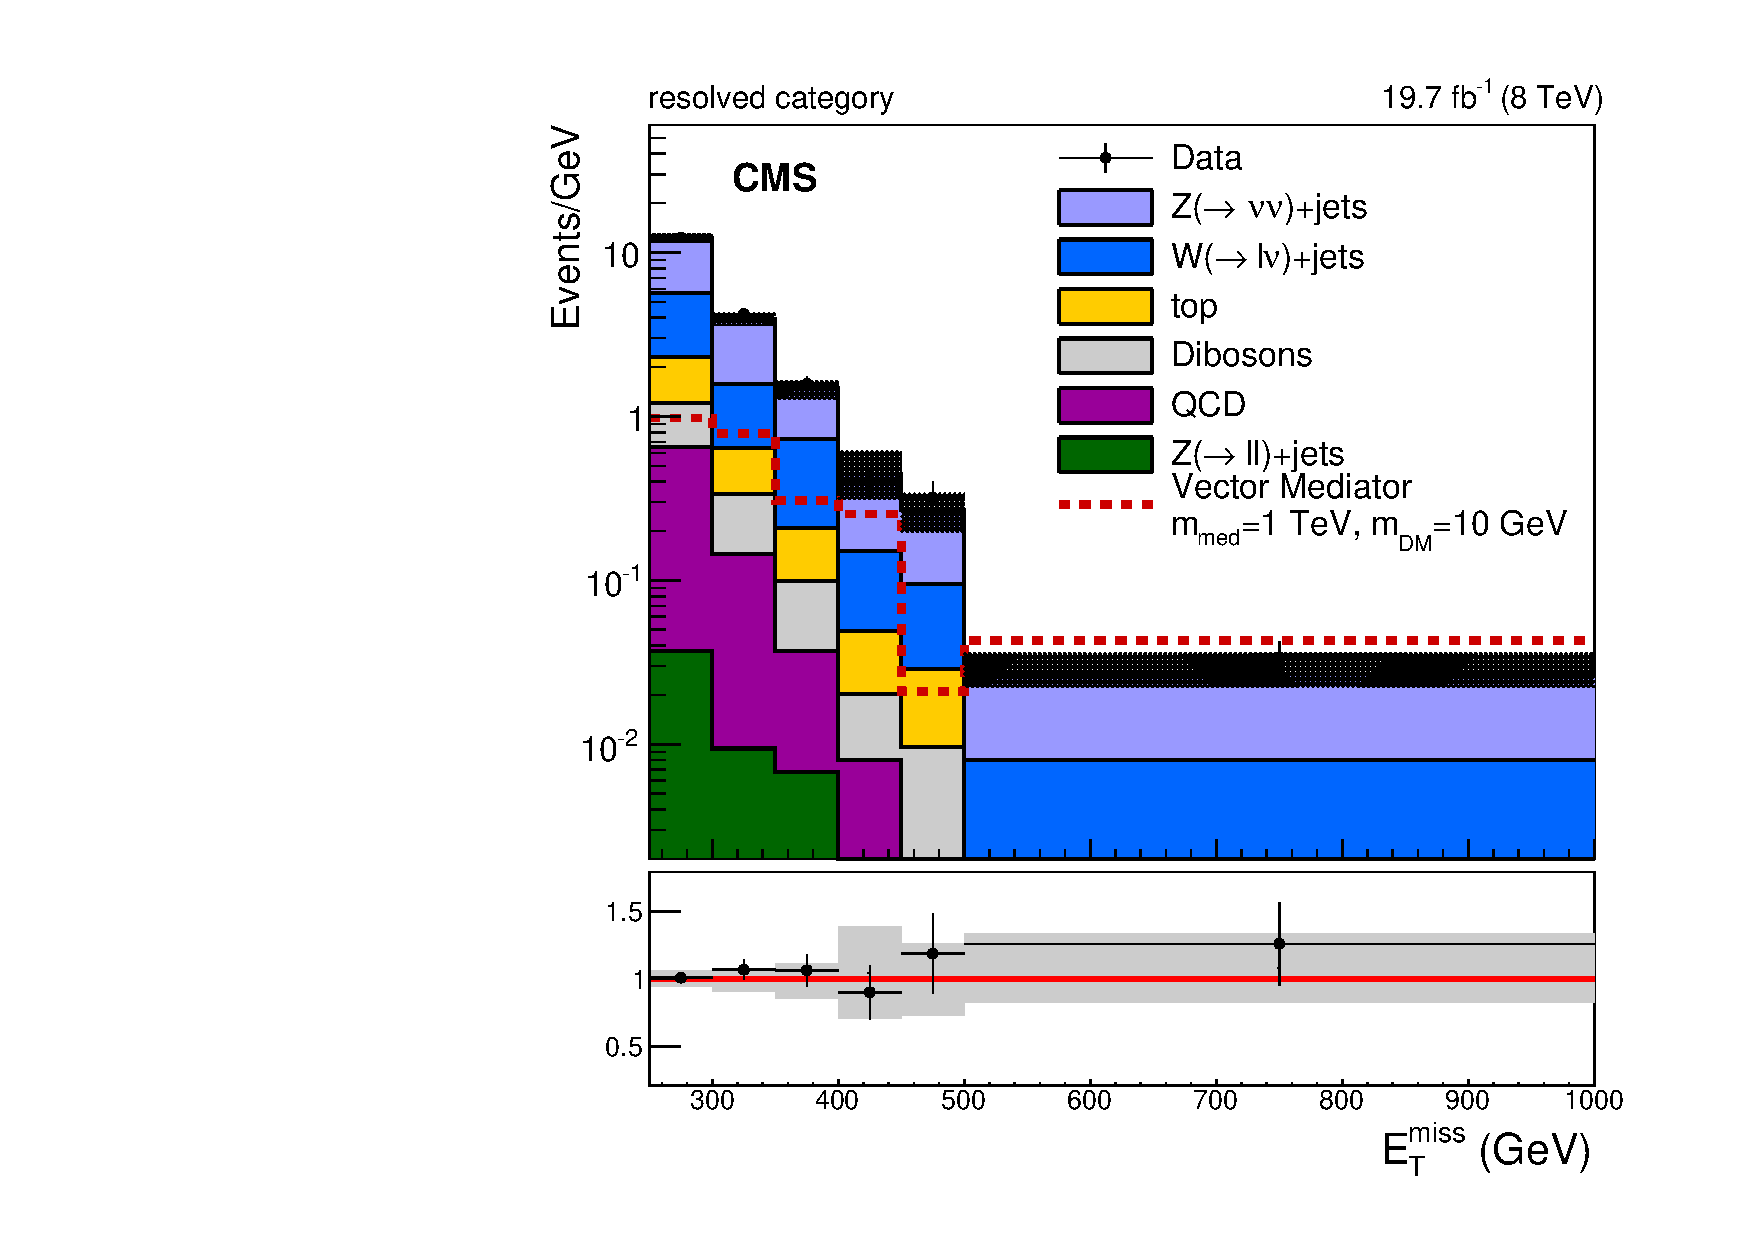
\includegraphics[width=0.5\textwidth]{figures/plot_config_resolved.pdf}
}\\
  \subfloat[][]{
 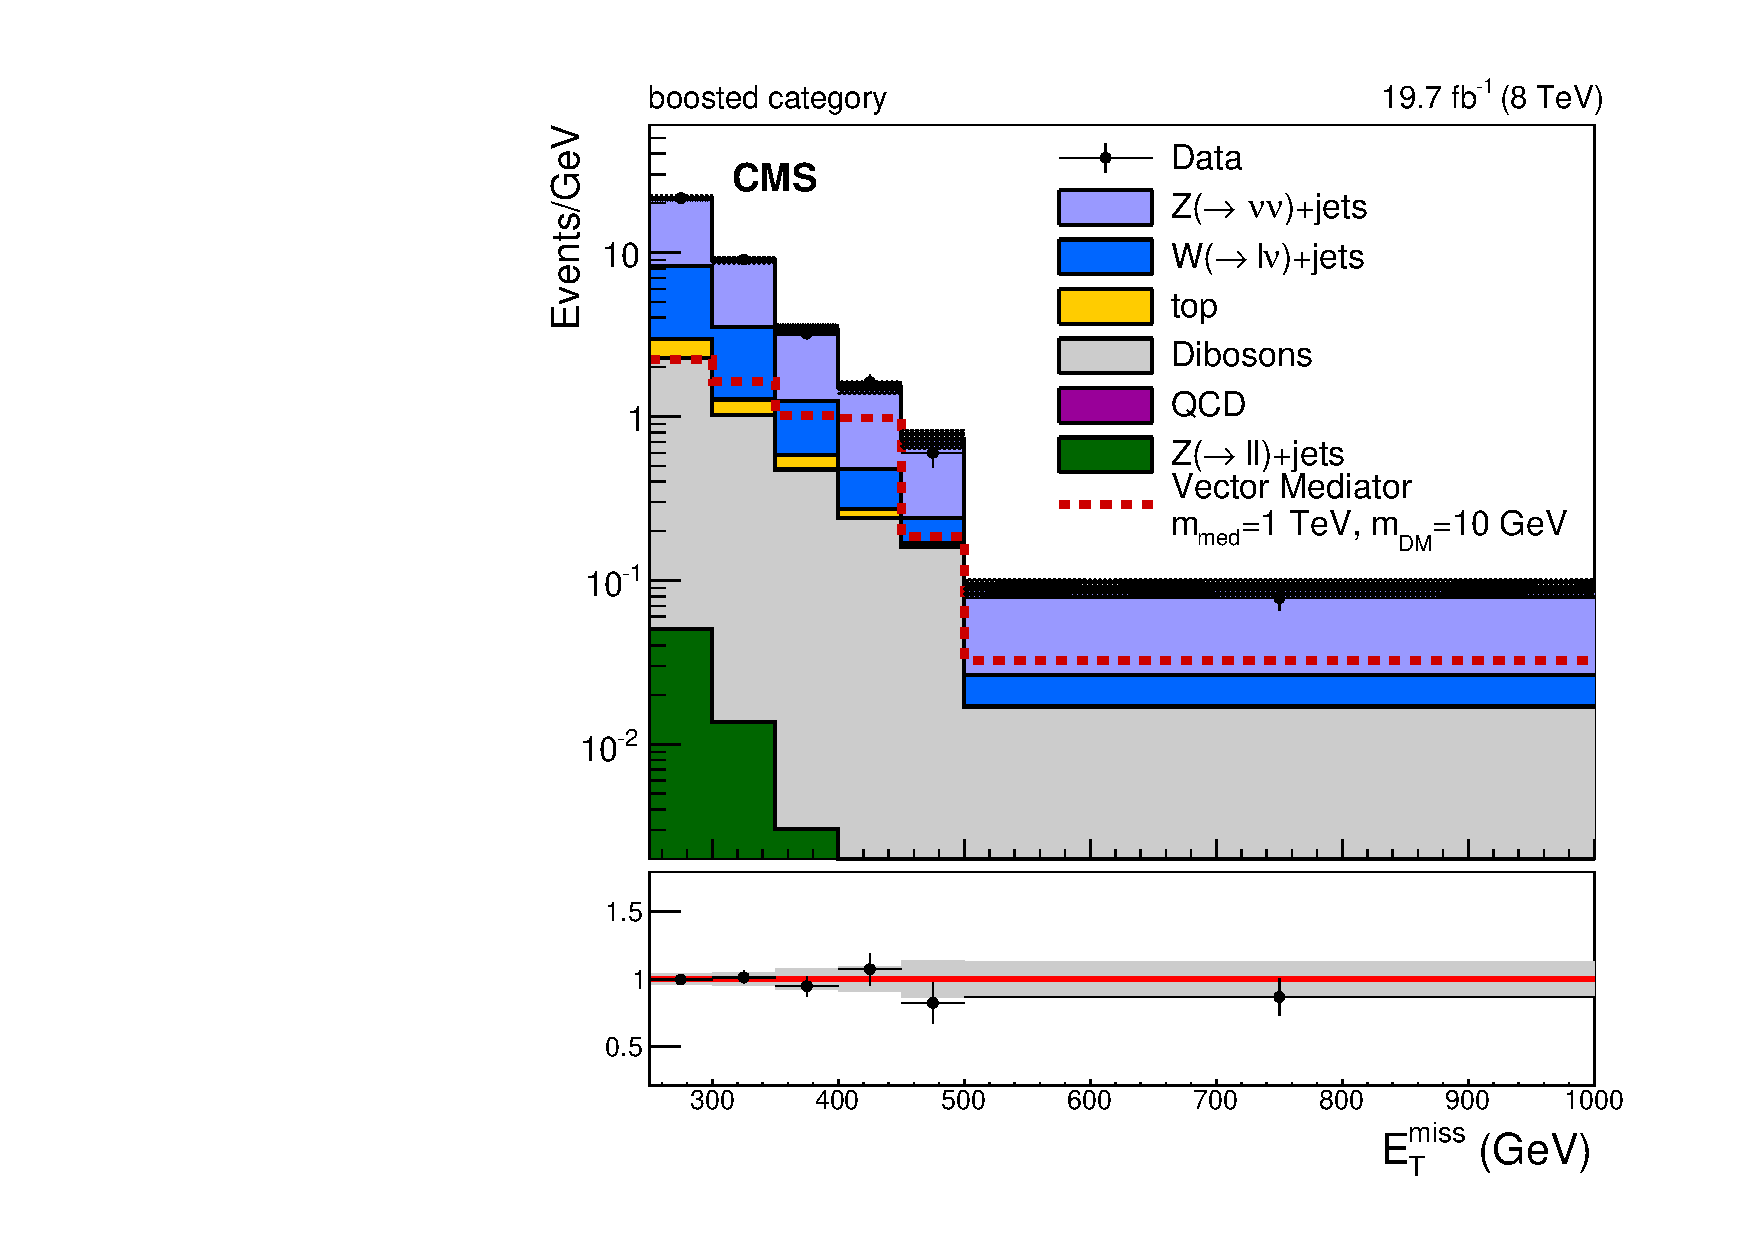
\includegraphics[width=0.5\textwidth]{figures/plot_config_boosted.pdf}
}
 \caption{
   Post-fit distributions of \ETm expected from SM backgrounds and observed in data in the signal region. The expected distributions are 
   evaluated after fitting to the observed data simultaneously across the monojet (a), resolved (b) and boosted (c) categories. 
   The gray bands indicate the post-fit uncertainty on the background, assuming no signal. The expected distribution assuming vector mediated DM production 
   is shown for a DM mass of 10 GeV and a mediator mass of 1 TeV.
 }
 \label{fig:post_fit_plots}\end{center}\end{figure*}

Exclusion limits are set for these models using the CLs method~\cite{cls} with a profile likelihood ratio as the 
test-statistic in which systematic uncertainties are modelled as nuisance parameters. 
For each signal hypothesis tested, upper limits are placed on the ratio of 
the signal cross-section to the predicted cross-section, denoted as $\mu=\sigma/\sigma_{TH}$. Limits are presented in terms of excluded regions in the 
$m_{\mathrm{MED}}-m_{\textrm{DM}}$ plane, assuming the four different mediators, by determining the points for which $\mu\ge1$ is excluded at 90\% CL or more.
Experimental systematic uncertainties, including jet and \ETm response and resolution, are included on the signal model as nuisance parameters, while the
theoretical systematic uncertainties on the inclusive cross-section (20\% and 30\% for the vector and axial-vector, and scalar and pseudoscalar models respectively) due to QCD scale and 
PDF uncertainties are instead added as additional contours to the exclusion limits. These uncertainties are chosen to be conservative across the full range in mediator mass.

To compare direct detection experiments with collider experiments, the direct detection bounds can be interpreted under the Lagrangians given in Equation~\ref{eq:LS}. The limits obtained in 
the simplified models use the standard approaches to compute t-channel scattering~\cite{Kurylov:2003ra,Hisano:2010ct, Cheung:2013pfa,Buchmueller:2014yoa}. 
For the vector and scalar mediator models, the limits are compared with the measurements by LUX~\cite{Akerib:2012ys,Akerib:2013tjd,Szydagis:2014xog} which currently 
provides the strongest constraints for $m_{\rm{DM}} \gtrsim 6$ GeV. For axial-vector couplings, the limits are compared with 
DM-proton-scattering limits from PICO-2L~\cite{Amole:2015lsj}..
For pseudoscalar interactions, direct detection bounds are strongly velocity suppressed. 
The most appropriate comparison is therefore to the most sensitive bounds from indirect detection from FermiLAT~\cite{Ackermann:2011wa,Abdo:2010ex}. 
These limits apply to the scenario in which dark matter is annihilated in the center of a galaxy producing a $\gamma$ ray signature. 
The results are also compared, for all four types of mediators, to constraints obtained from the observed cosmological relic density of DM as determined from 
measurements of the cosmic microwave background by the WMAP and Planck experiments~\cite{Bennett:2003ba,Planck:2006aa}. The expected DM abundance is estimated, separately for each
model, using a thermal freeze-out mechanism implemented in MadDM~\cite{Backovic:2013dpa}, and compared to the observed cold DM density $\Omega_c*h^2=0.12$~\cite{Ade:2013zuv}. 
It is assumed that the simplified model hypothesised provides the only relevant BSM dynamics for DM interactions.

Figure~\ref{fig:masslims} shows the 90\% CL exclusions for the vector, axial-vector, 
scalar and pseudoscalar mediator models.  The 90\% confidence level upper limit on the ratio of excluded cross-section to the predicted cross-section ($\mu_{\textrm{up}}$), 
when assuming the mediator only couples to fermions, is shown by the blue color scale. These limits are calculated under the assumption 
that only the initial state partons and the DM 
particle contribute to the width of the mediator. For all models, the width is fixed under the minimum width constraint~\cite{An:2012va,Abercrombie:2015wmb,Fox:2011pm,simplified1}. 
%For the vector mediator, the direct-detection bounds dominate above $m_{DM}=6$~\GeV, while for the axial-vector, scalar, pseudoscalar mediator models, the bounds 
%
Under the vector mediator model, the direct detection bounds dominate across most of the plane, while for the axial-vector, there is good complementarity between the direct detection limits and 
those from this analysis. Limits in the scalar mediator scenario are more sensitive than those from direct detection for small dark-matter masses. Additional sensitivity is gained
for larger mediator masses in this scenario above 350 \GeV due to the rise in cross-section of the gluon fusion loop process above the $t\bar{t}$ threshold. 
In the pseudoscalar mediator scenario, the limits from this analysis exceed the reach in $m_{\mathrm{MED}}$ than those from FermiLAT over the whole region.

\begin{figure}[htbp]
  \centering
  \subfloat[][]{
	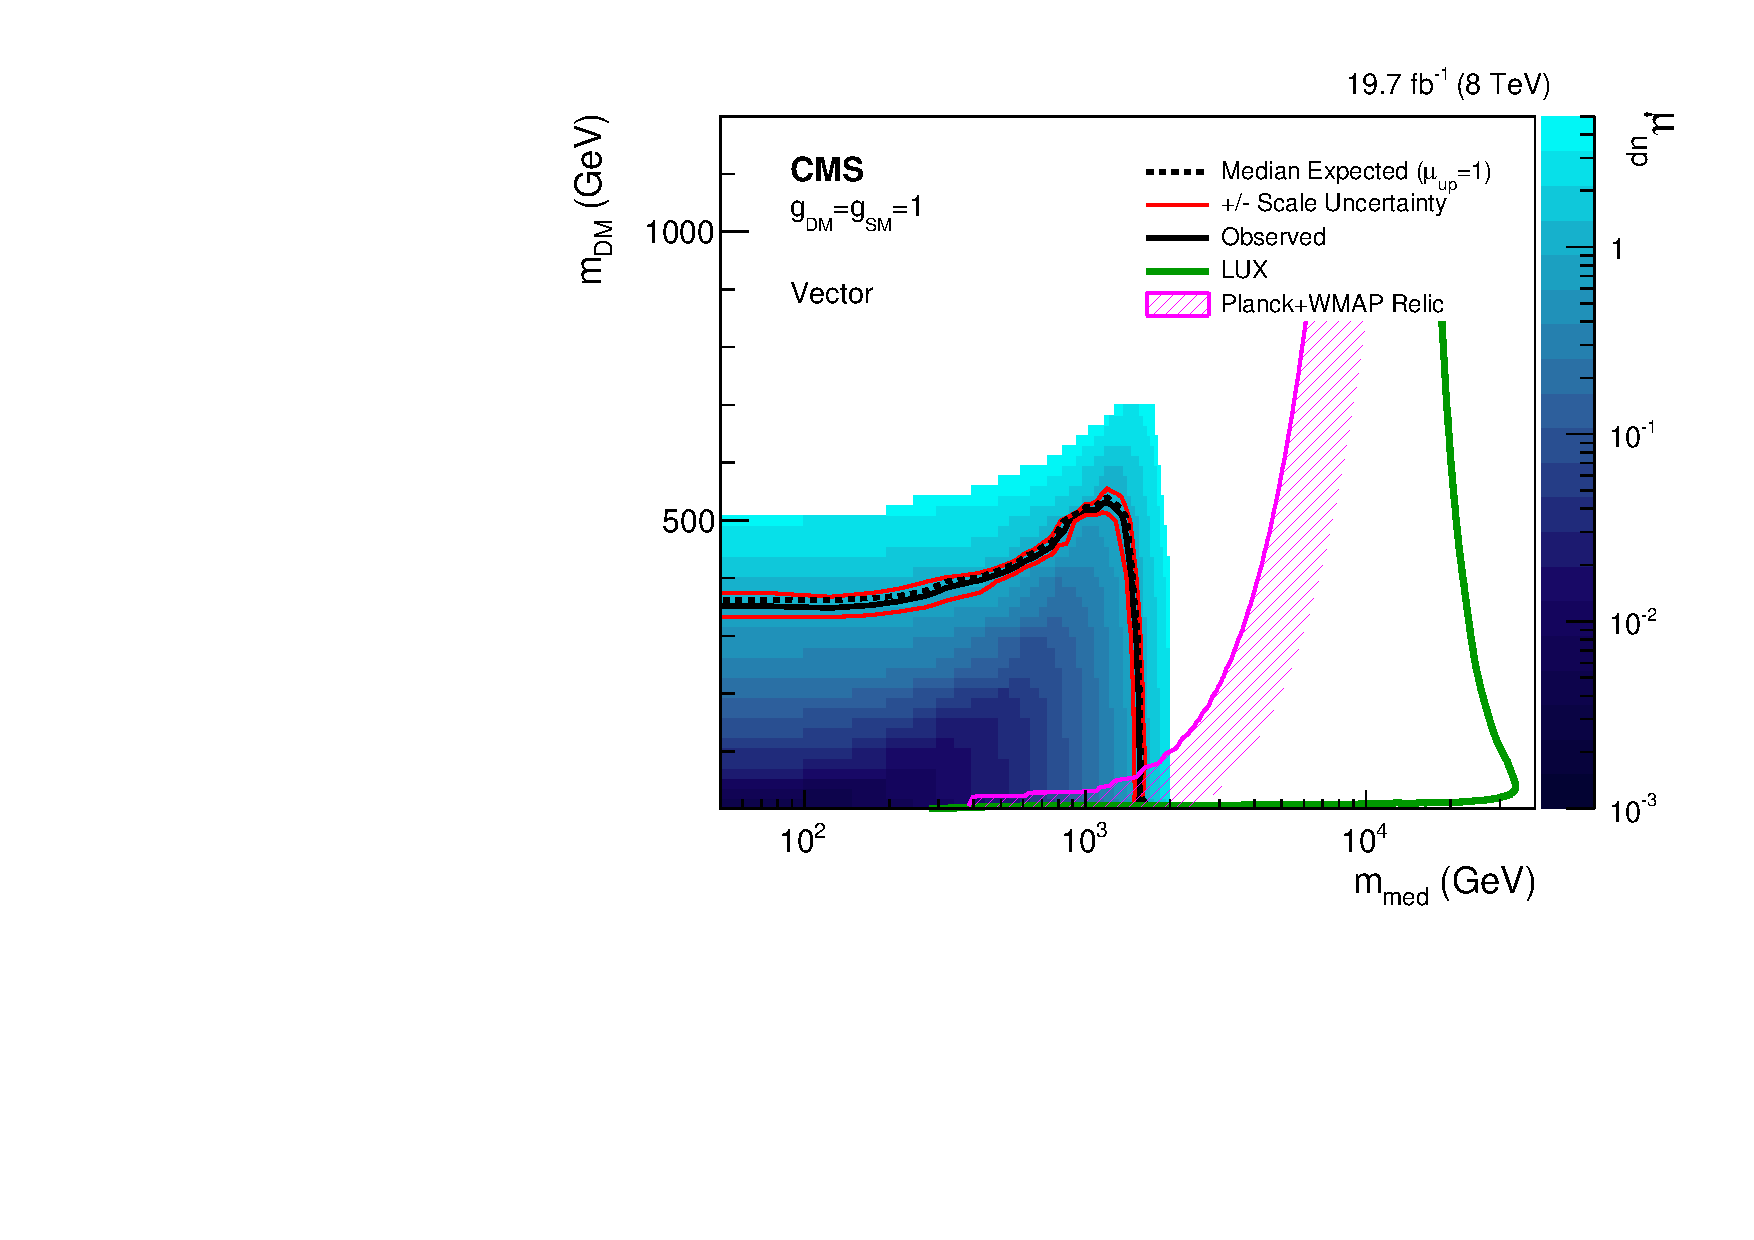
\includegraphics[angle=0,width=0.50\textwidth]{figures/MassLimit_1_800_0_Both.pdf}
	\label{fig:mass_800}
  }
  \subfloat[][]{
	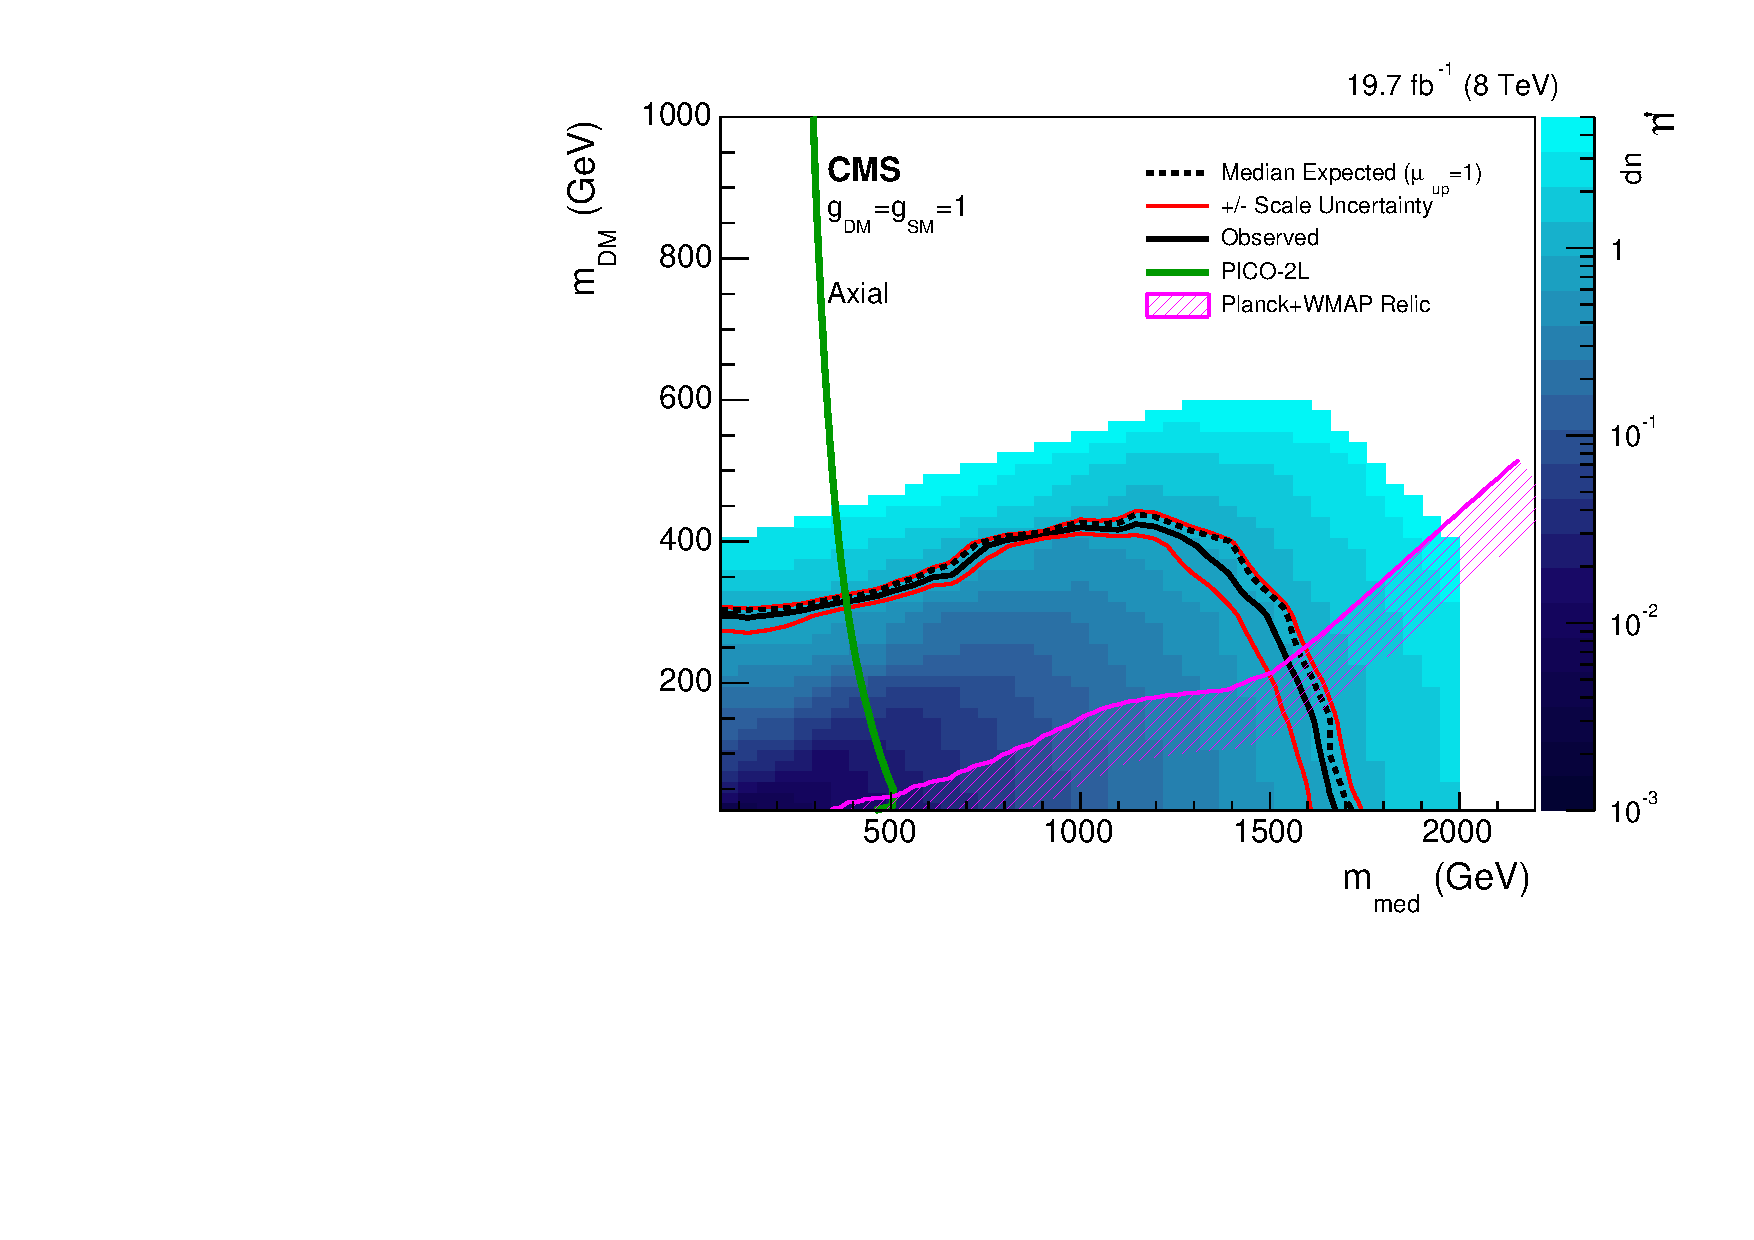
\includegraphics[angle=0,width=0.50\textwidth]{figures/MassLimit_1_801_0_Both.pdf}
	\label{fig:mass_801}
  }\\
  \subfloat[][]{
	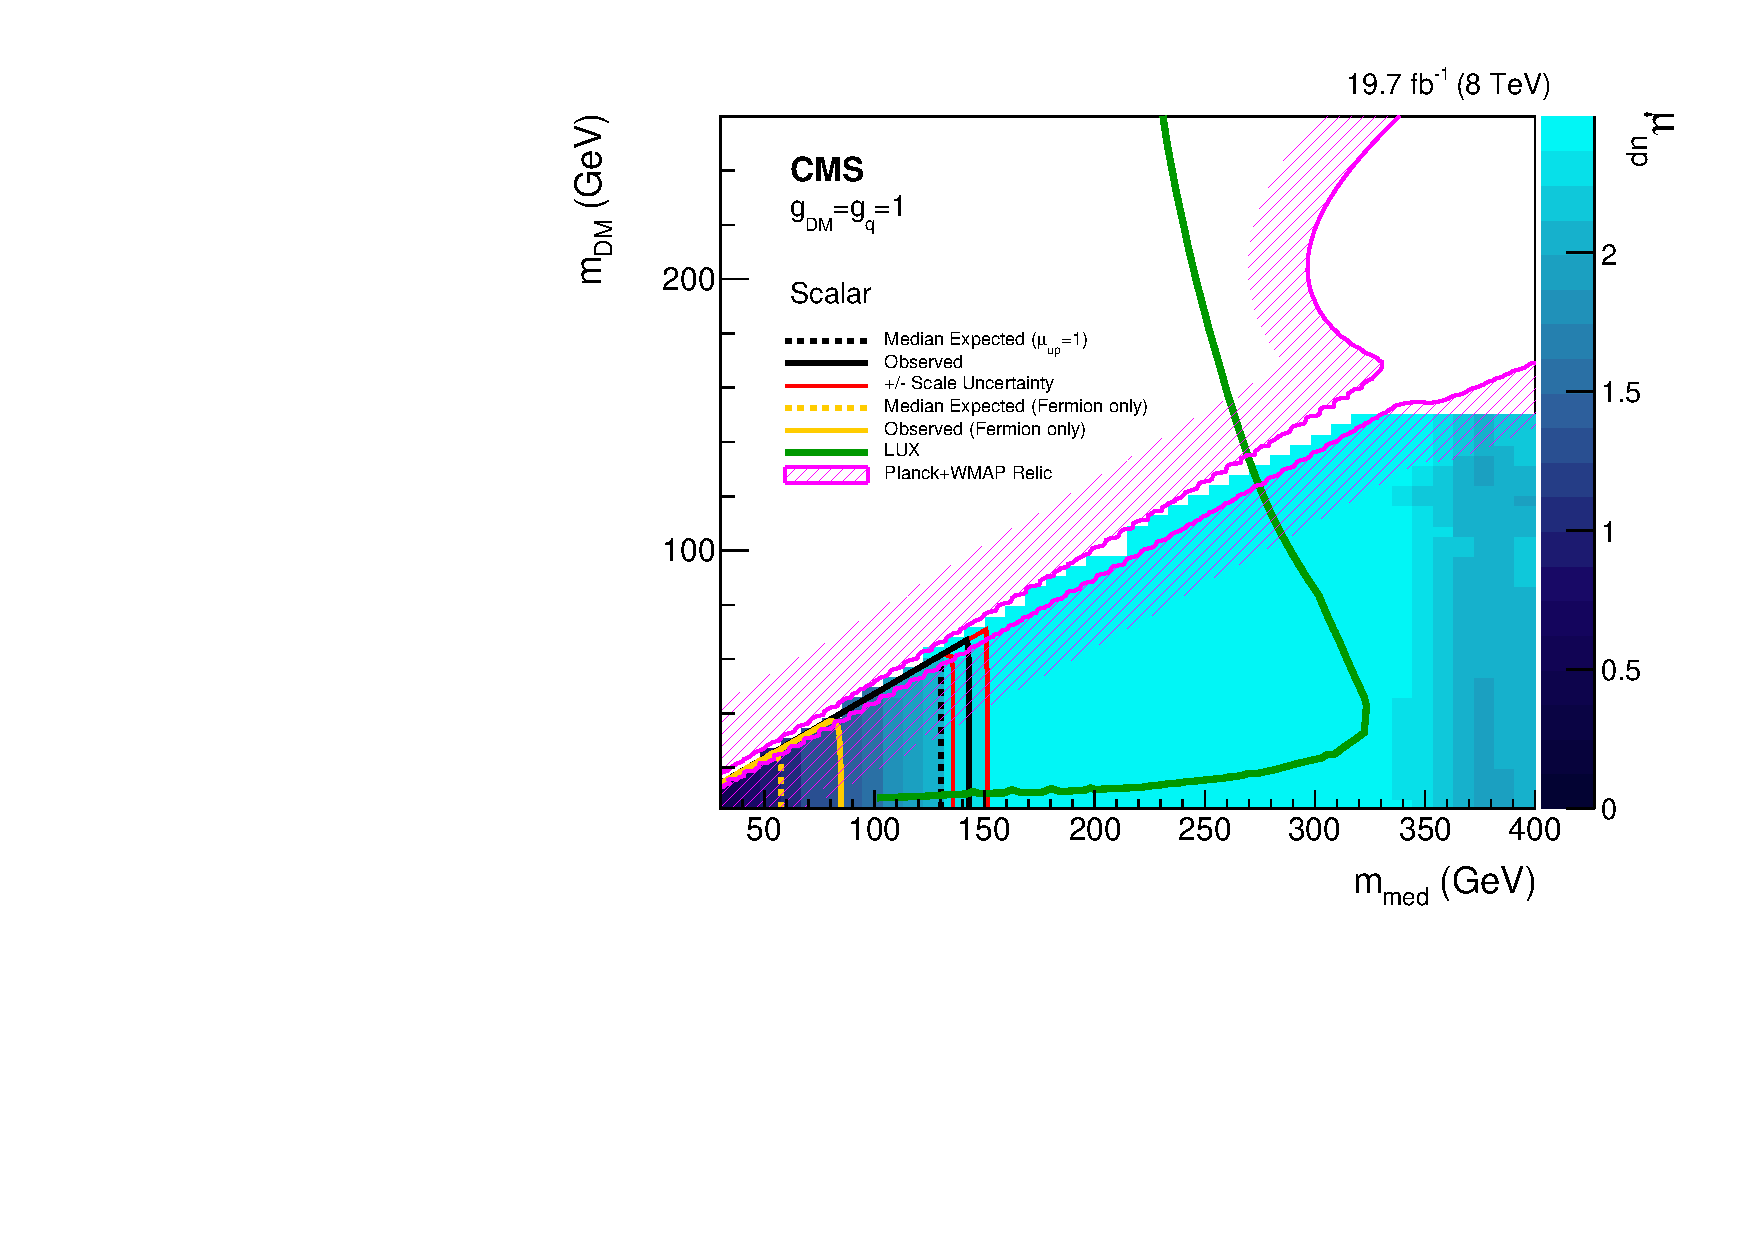
\includegraphics[angle=0,width=0.50\textwidth]{figures/MassLimit_1_805_0_Both.pdf}
	\label{fig:mass_805}
  }
  \subfloat[][]{
	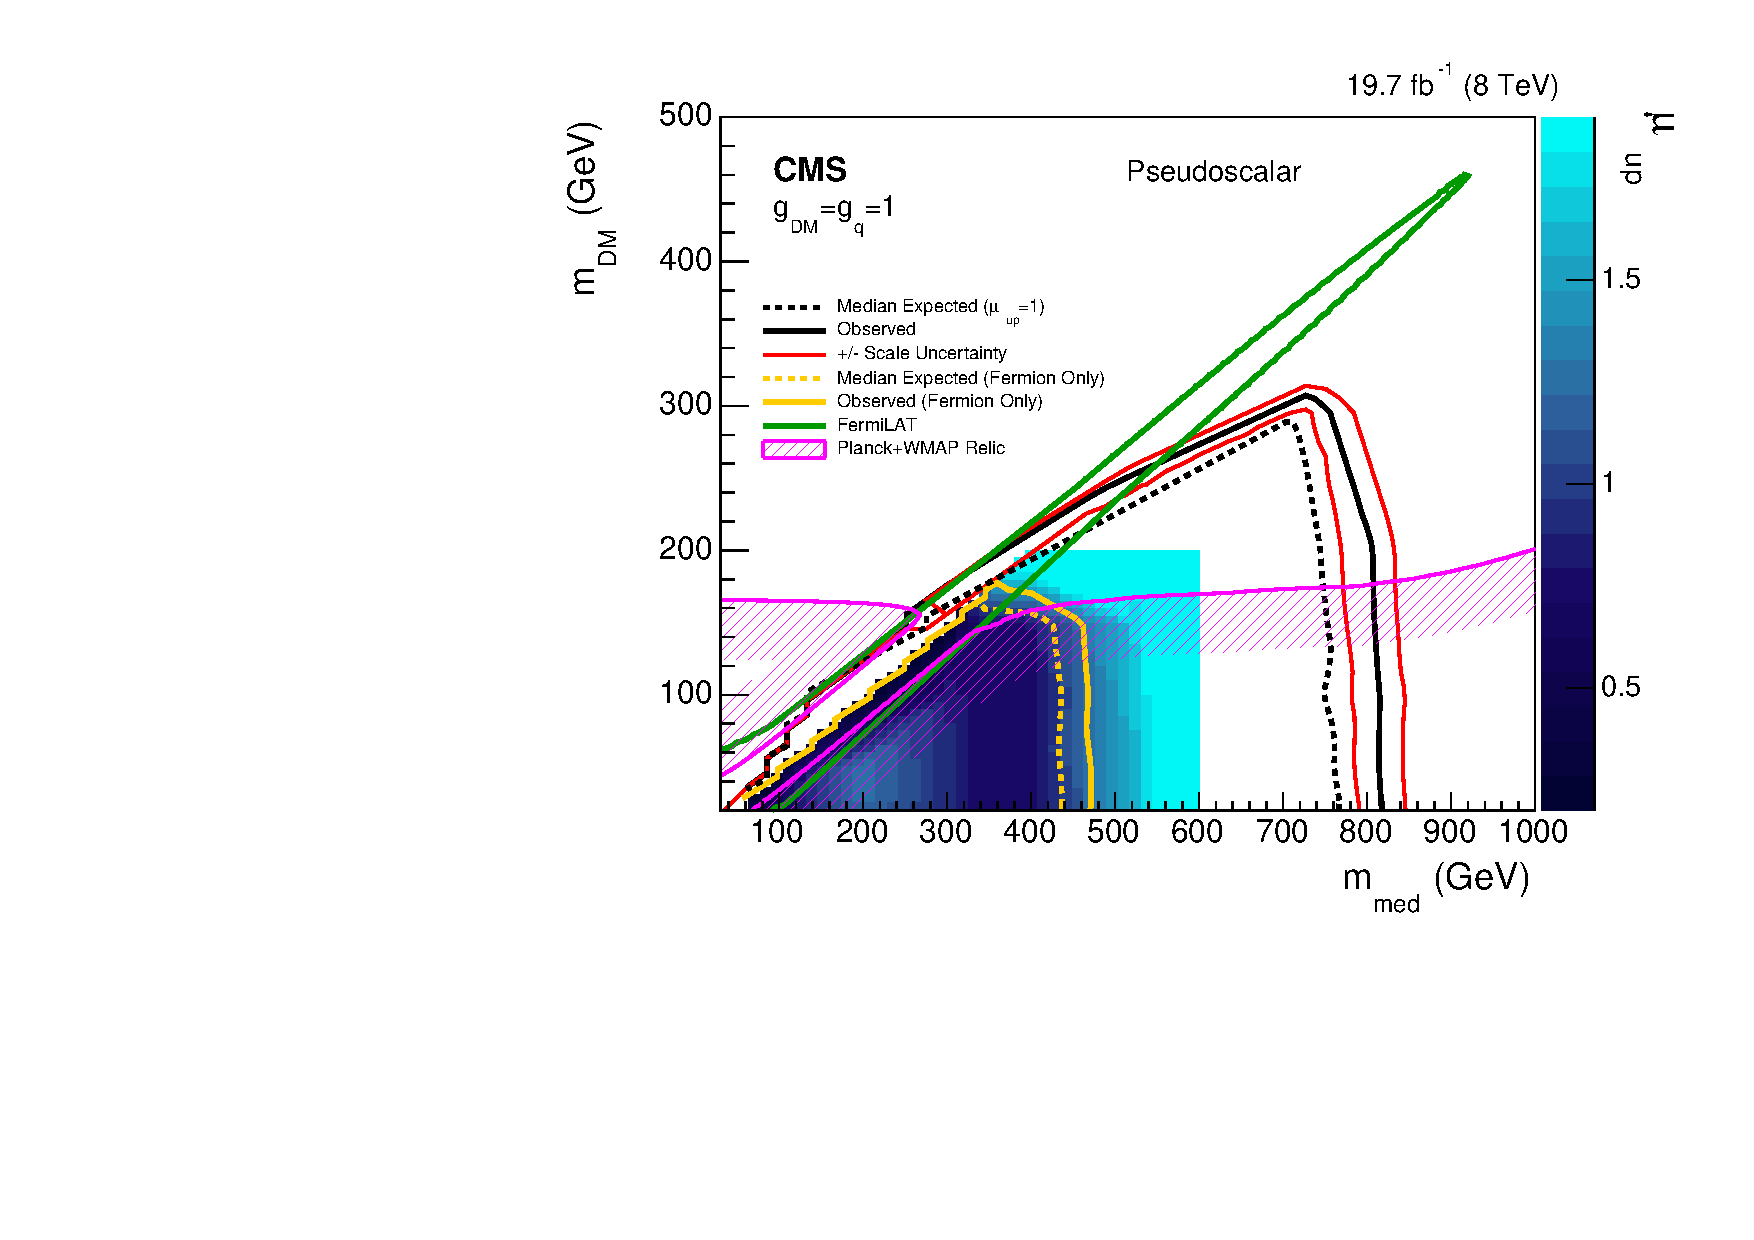
\includegraphics[angle=0,width=0.50\textwidth]{figures/MassLimit_1_806_0_Both.pdf}
	\label{fig:mass_806}
  }
  \caption{90\% CL Exclusion contours in the $m_{\textrm{med}}-m_{\textrm{DM}}$ plane assuming a vector (a), axial-vector (b), scalar (c), or pseudoscalar (d) mediator. 
The blue scale shows the 90\% CL upper limit on the signal strength assuming the mediator only couples to fermions. For the scalar and pseudoscalar mediators, the exclusion 
contour assuming coupling only to fermions is explicitly shown in the orange line. The white region shows model points which were not tested when assuming coupling only 
to fermions and are not expected to be excluded by this analysis under this assumption.
The excluded region is to the bottom-left of the contours shown in all cases except for that from the relic density as indicated by the shading.
In all of the mediator models, a minimum width is assumed\label{fig:masslims}.}
\end{figure}


%Figures~\ref{fig:xslims_800},~\ref{fig:xslims_801} and~\ref{fig:xslims_805} show the same exclusion contours, this time translated into the 
%plane of $m_{\textrm{DM}}-\sigma_{\textrm{DD}}$, where $\sigma_{\textrm{DM}}$ is 
%the spin-independent/dependant (vector and scalar/axial-vector) DM-nucleon scattering cross-section. 
%These representations allow for a more direct comparison with the direct-detection expedients which typically set 
%model-independent limits on these cross-sections. It should be noted that the limits set from this 
%analysis are however only valid under the simplified model considered, and in particular 
%assuming $g_{DM}=g_{SM}=1$. For the scalar model, it is assumed that only heavy quarks 
%(top and bottom) contribute. Such a choice limits the sensitivity for direct 
%detection, however it allows for direct comparison between collider and direct detection without an additional assumptions 

%on the light quark couplings~\cite{Harris:2015kda}.
Figures~\ref{fig:xslims_800},~\ref{fig:xslims_801} and~\ref{fig:xslims_805} show the same exclusion contours, this time translated into the 
plane of $m_{\textrm{DM}}-\sigma_{\textrm{SI/SD}}$, where $\sigma_{\textrm{SI/SD}}$ are 
the spin-independent/dependant (vector and scalar/axial-vector) DM-nucleon scattering 
cross-sections. These representations allow for a more direct comparison with limits from the direct-detection experiments which typically set 
upper limits on these cross-sections~\cite{ Malik:2014ggr,Harris:2015kda}. It should be noted that the limits set from this 
analysis are however only valid under the simplified model considered, and in particular 
assuming $g_{\textrm{DM}}=g_{\textrm{SM}}=1$. For the scalar model, it is assumed that only heavy quarks 
(top and bottom) contribute. Such a choice limits the sensitivity for direct 
detection, however it allows for direct comparison between collider and direct detection without an additional assumption 
on the light quark couplings~\cite{Harris:2015kda}.  
For the vector and scalar mediator models, direct-detection limits are stronger than 
those obtained in this analysis except in the scenario where the dark matter mass is less than around 6 \GeV while for the axial-vector mediator model, the 
limits obtained in this analysis dominate up to around $m_{\mathrm{DM}}=300$ \GeV. 
 
The excess observed in FermiLAT data has led to speculations that dark matter annihilation is mediated by a light pseudoscalar~\cite{Calore:2014nla}. 
The production mechanism for these $\gamma$ rays can be interpreted under dark matter annihilation to b-quarks allowing for direct 
comparison with limits from this analysis~\cite{Buchmueller:2015eea,Buckley:2014fba,Harris:2014hga}. Figure~\ref{fig:xslims_806} shows 
the exclusion contours assuming pseudoscalar mediation in the plane of DM pair annihilation cross-section versus $m_{\textrm{DM}}$. 
It is assumed that only heavy quarks (top and bottom quarks) contribute in the production of the mediator while for  
the interpretation of the limits in the annihilation cross-section, it is assumed that the mediator only decays to b-quark pairs. 
%Such a choice limits the sensitivity for direct 
%detection, however it allows for direct comparison between collider and direct detection without an additional assumptions 
%on the light quark couplings~\cite{Harris:2015kda}. 
As with all interpretations, the DM particle is assumed to be a Dirac fermion.
The 68\% CL preferred regions in this plane assuming the annihilation of DM pairs to light-quarks (qq), tau or bottom pairs, using data from FermiLAT, 
are shown as solid colour regions. Under the simplified model used, all of these regions are excluded by this analysis.

%\begin{figure}[htbp]
%  \centering
%	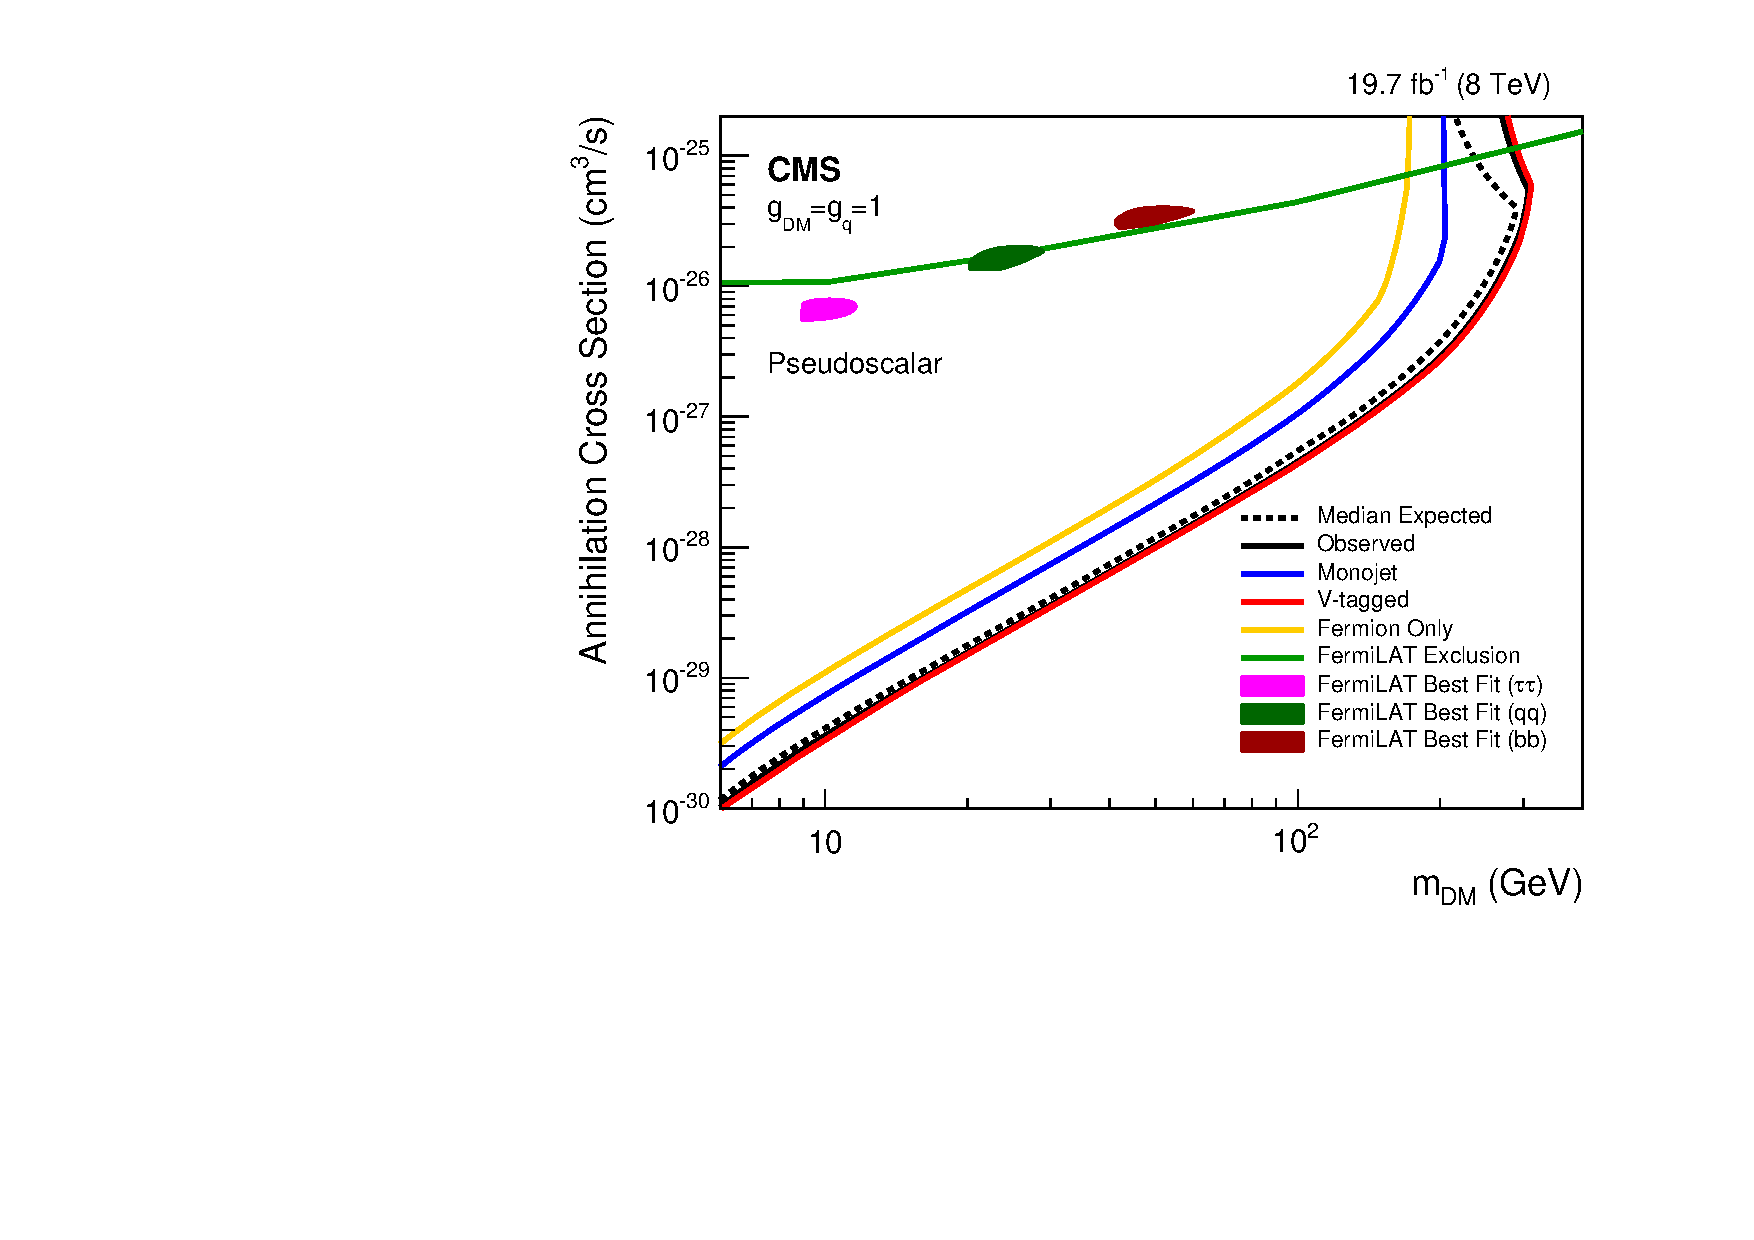
\includegraphics[angle=0,width=0.70\textwidth]{figures/MassLimit_1_806_0_Both_DD.pdf}
%  \caption{90\% CL Exclusion contours in the $m_{\textrm{med}}-\sigma_{\textrm{DM}}$ plane assuming a pseudoscalar mediator. 
%The orange line shows the exclusion contours assuming the mediator only couples to fermions. 68\% CL preferred regions, using data from FermiLAT, for DM annihilation 
%to light-quarks (qq), tau pairs ($\tau\tau$) and bottom-quark pairs (bb) are shown by the solid green, pink and brown coloured regions respectively.\label{fig:xslims}}
%\end{figure}

\begin{figure}[htbp]
  \centering
  \subfloat[][]{
	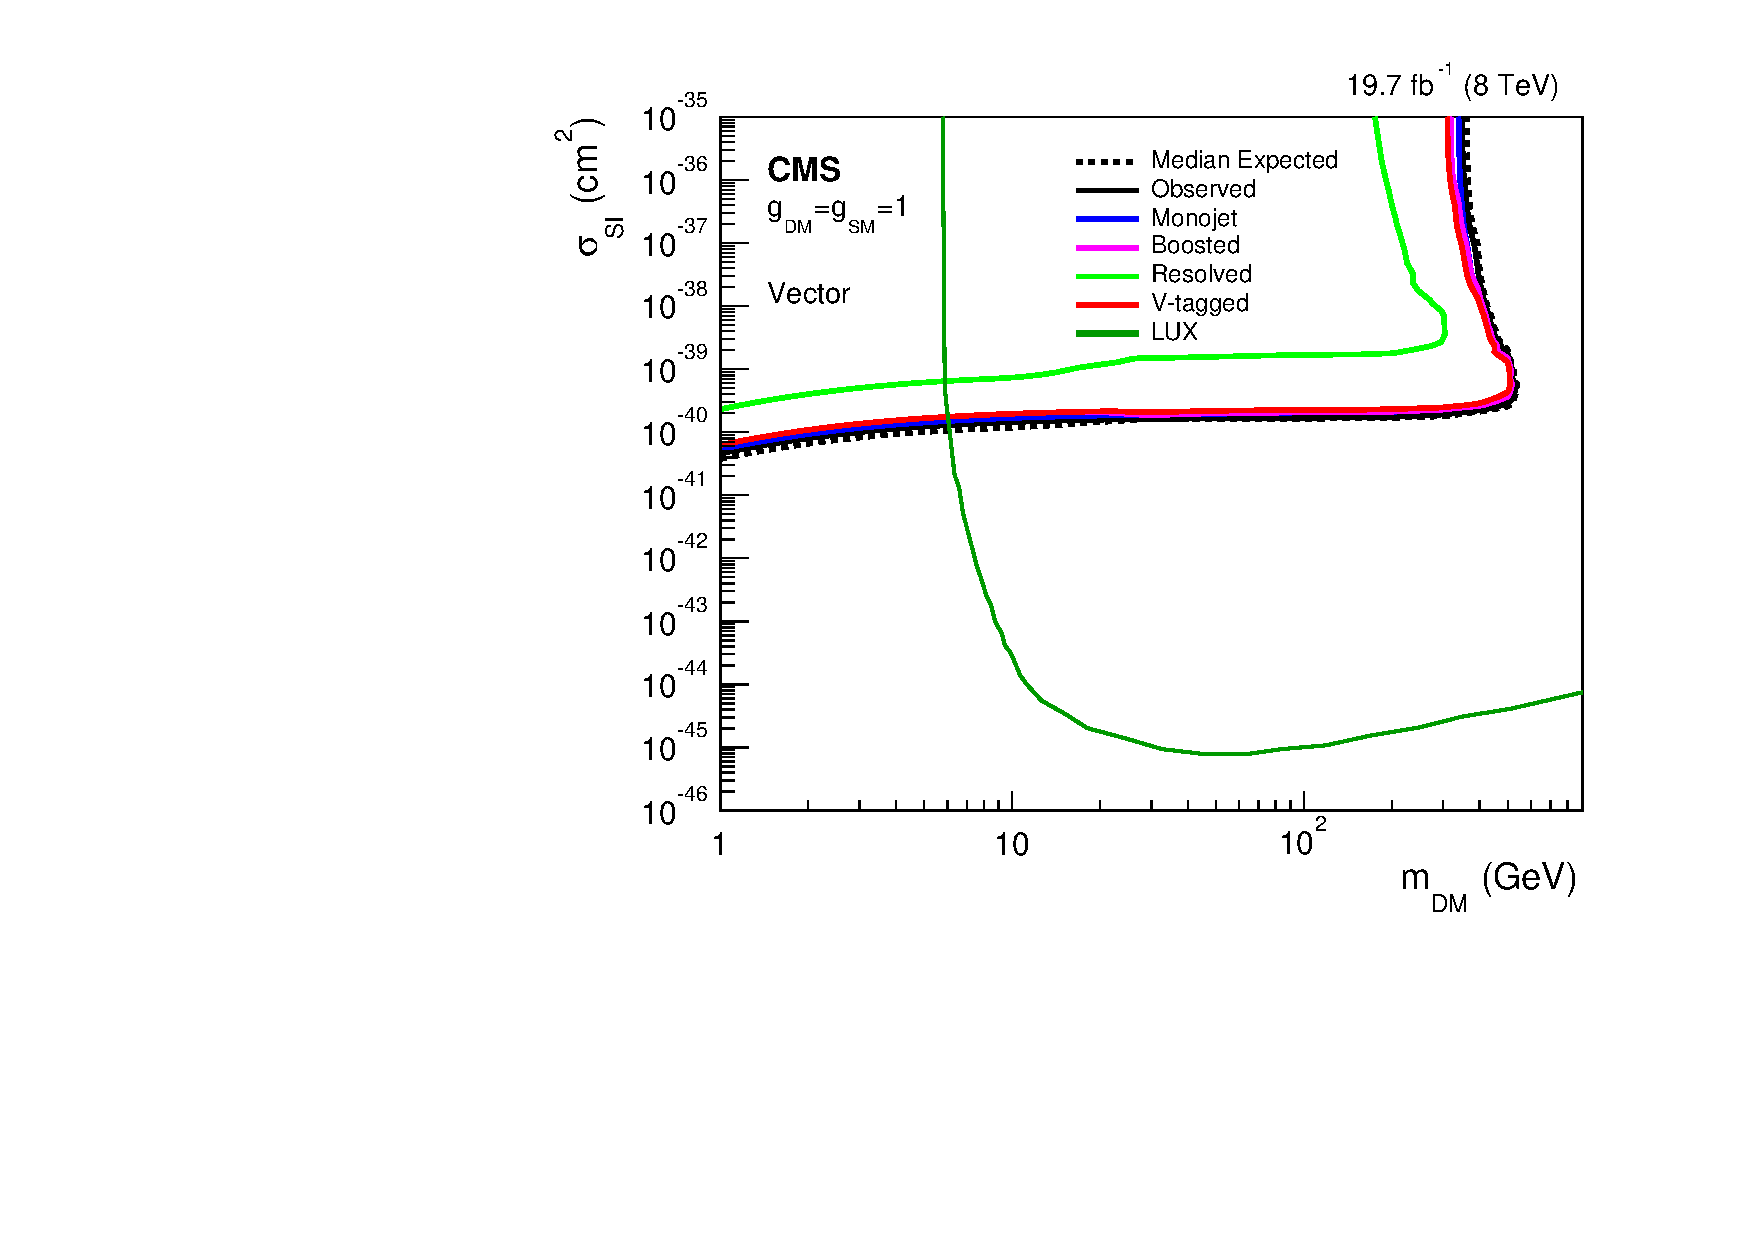
\includegraphics[angle=0,width=0.50\textwidth]{figures/MassLimit_1_800_0_Both_DD.pdf}
	\label{fig:xslims_800}
  }
  \subfloat[][]{
	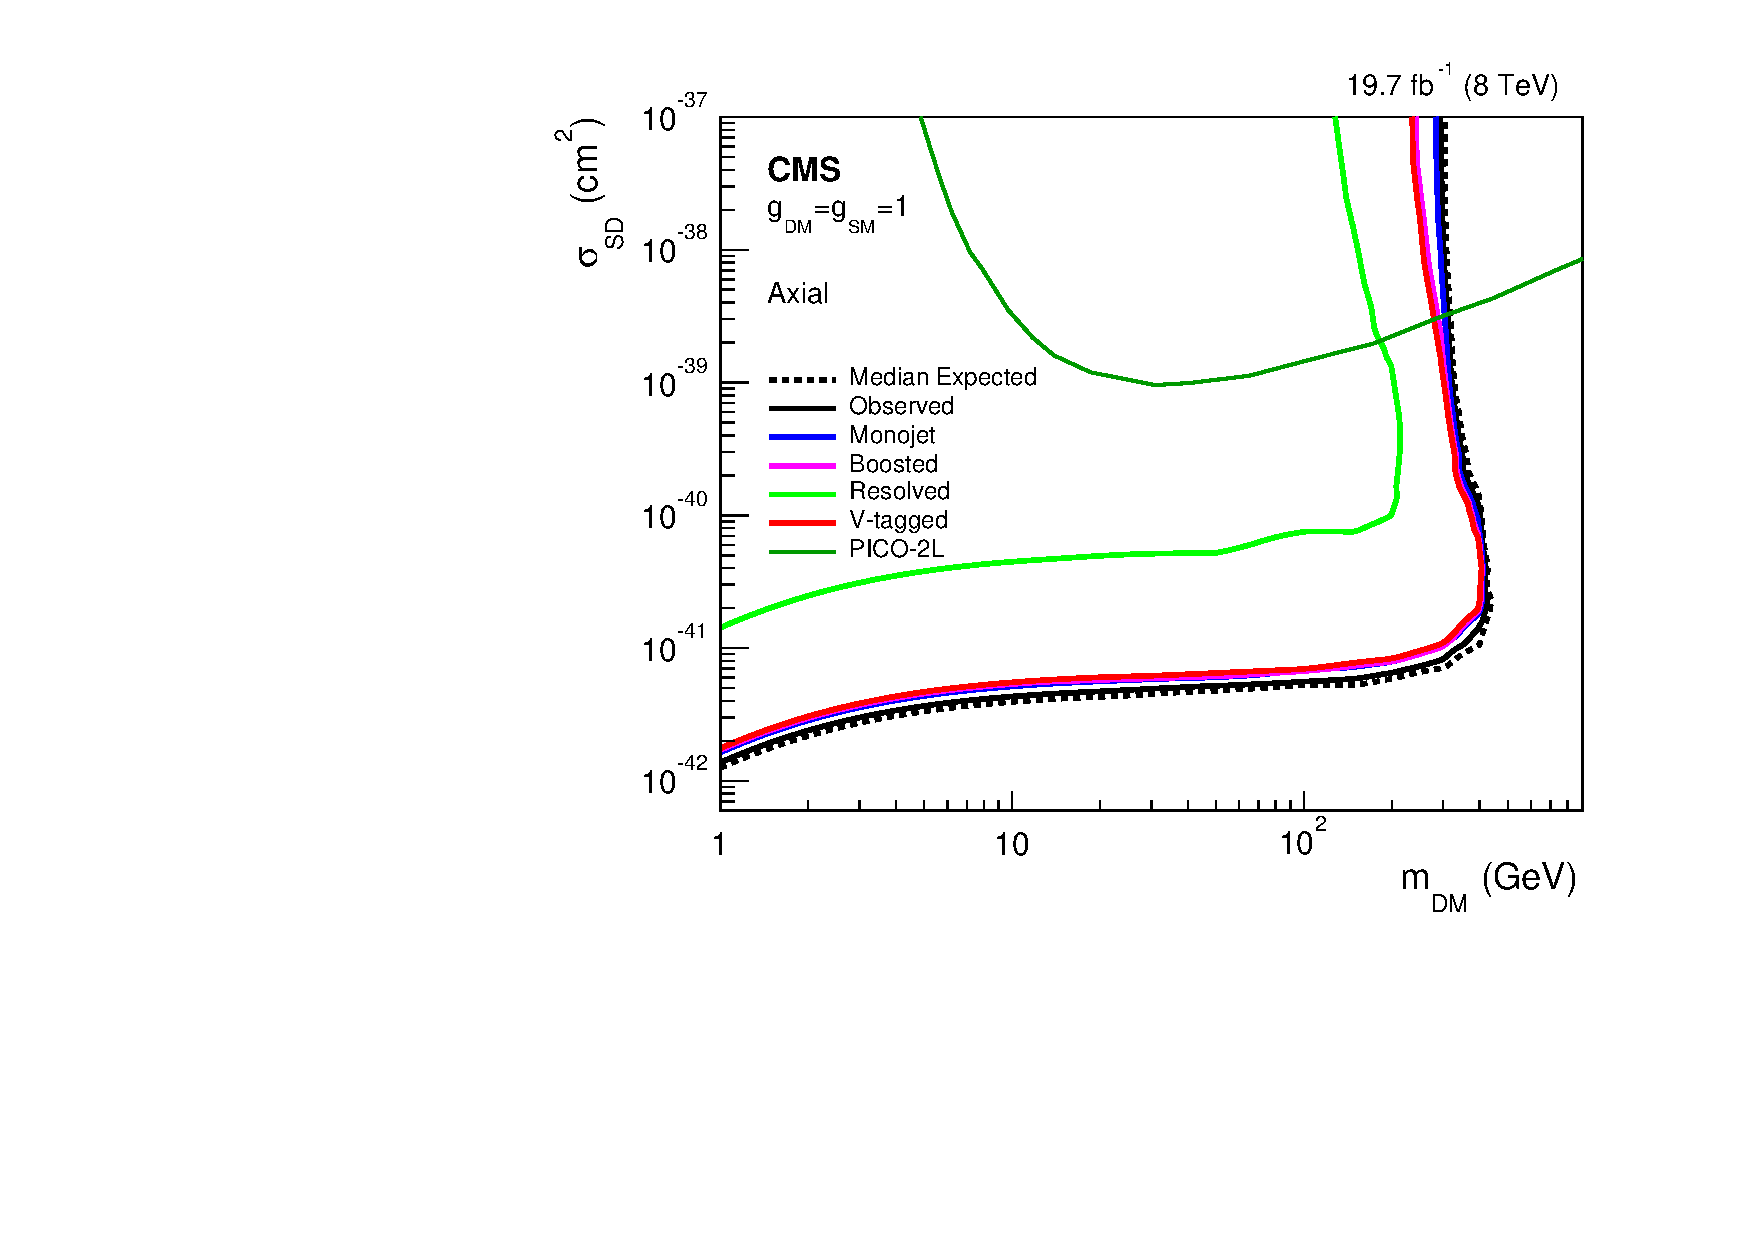
\includegraphics[angle=0,width=0.50\textwidth]{figures/MassLimit_1_801_0_Both_DD.pdf}
	\label{fig:xslims_801}
  }\\
  \subfloat[][]{
	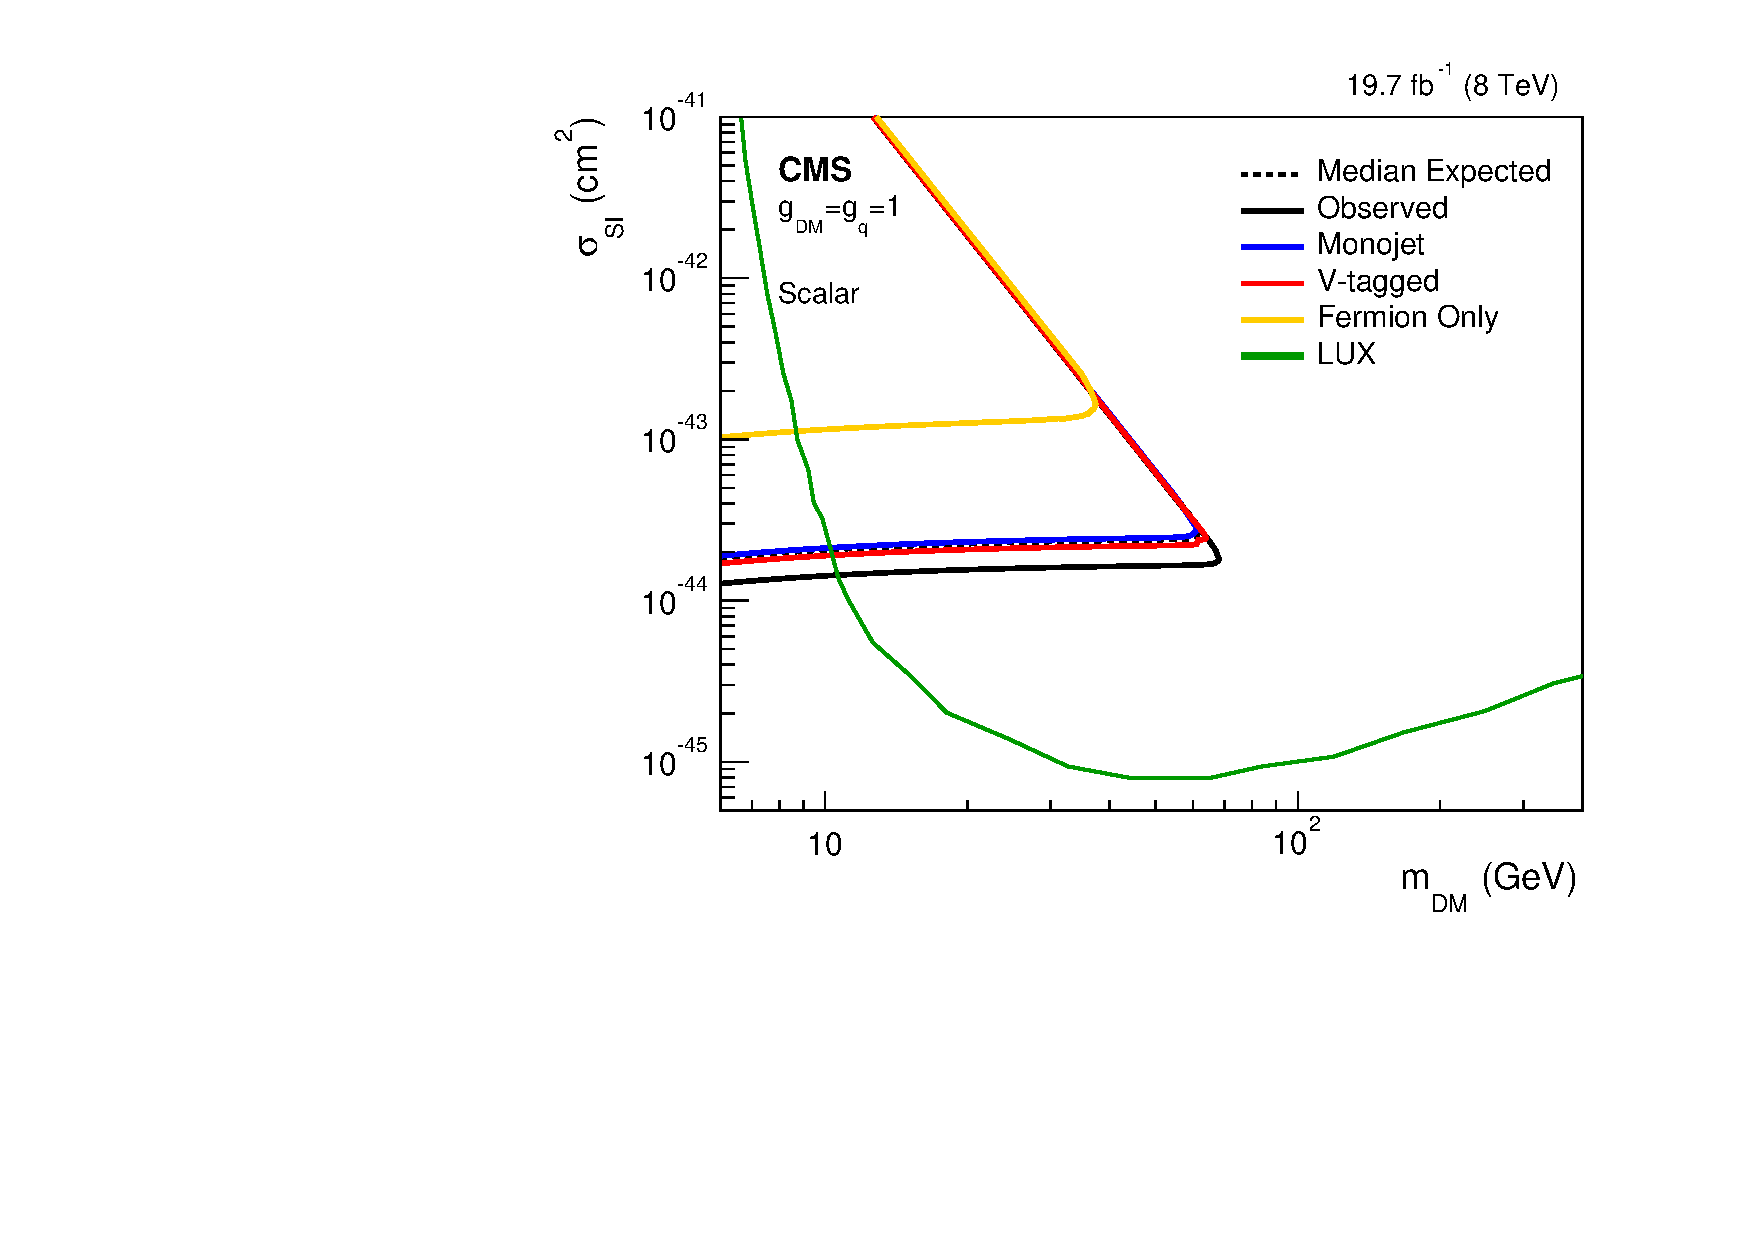
\includegraphics[angle=0,width=0.50\textwidth]{figures/MassLimit_1_805_0_Both_DD.pdf}
	\label{fig:xslims_805}
  }
  \subfloat[][]{
	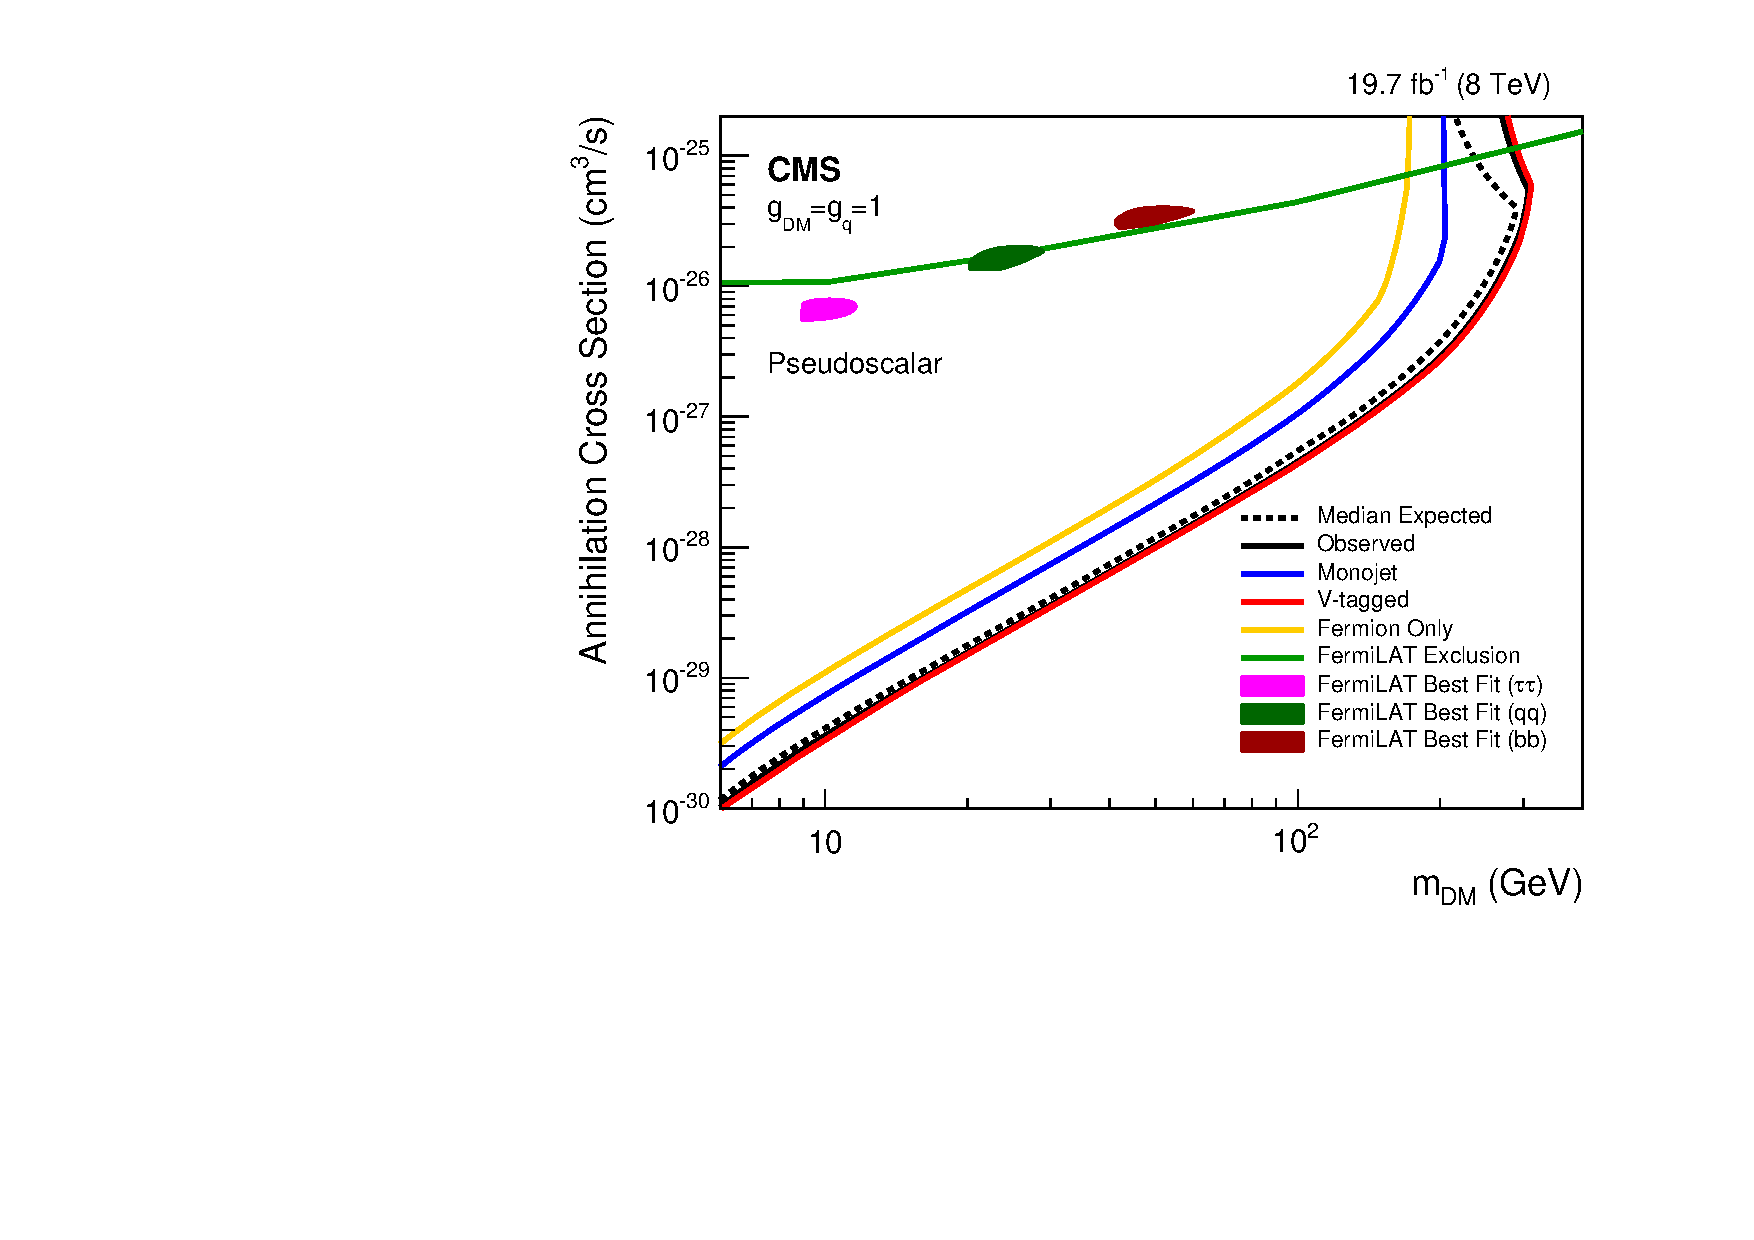
\includegraphics[angle=0,width=0.50\textwidth]{figures/MassLimit_1_806_0_Both_DD.pdf}
	\label{fig:xslims_806}
  }
  \caption{90\% CL Exclusion contours in the $m_{\textrm{DM}}-\sigma_{\textrm{DM}}$ plane assuming a vector (a), axial-vector (b), scalar (c), or pseudoscalar (d) mediator. 
For the scalar and pseudoscalar case, the orange line shows the exclusion contours assuming the mediator only couples to fermions. The excluded region in all plots is to the top 
left of the contours shown. In the vector and axial-vector scenarios, limits are shown independently for monojet, boosted and resolved categories. The partial combination of 
the "V-tagged" categories (resolved and boosted) categories is shown for which the boosted category provides the dominant contribution.
In all of the mediator models, a minimum width is assumed. For the pseudoscalar, 68\% CL preferred regions, using data from FermiLAT, for DM annihilation 
to light-quarks (qq), tau pairs ($\tau\tau$) and bottom-quark pairs (bb) are shown by the solid green, pink and brown coloured regions respectively. }
\end{figure}


\section{Summary}
A search has been presented for an excess of events with a high energy jet 
in association with a large missing transverse momentum in a data sample of 
proton-proton interactions at centre-of-mass energy of 8 TeV. The data 
correspond to an integrated luminosity of 19.7\fbinv collected by the CMS 
detector at the LHC. Sensitivity to mono-V models is achieved by tagging events 
consistent with the jet originating from a hadronically decaying vector boson. 
No significant deviation from the expectation from SM backgrounds is observed in the \ETm 
distributions.  
The search is interpreted in terms of DM production to place 
constraints on the parameter space of the simplified models considered. 

\clearpage
%\appendix
%\input{appendix}
%%%%%%%%%%%%%%%%%%%%%%%%%%%%%%%%  Begin text %%%%%%%%%%%%%%%%%%%%%%%%%%%%%
%% **DO NOT REMOVE THE BIBLIOGRAPHY** which is located before the appendix.
%% You can take the text between here and the bibiliography as an example which you should replace with the actual text of your document.
%% If you include other TeX files, be sure to use "\input{filename}" rather than "\input filename".
%% The latter works for you, but our parser looks for the braces and will break when uploading the document.
%%%%%%%%%%%%%%%

%% **DO NOT REMOVE BIBLIOGRAPHY**
\bibliography{auto_generated}   % will be created by the tdr script.

%%% DO NOT ADD \end{document}!

